\bookpart{拓扑与度量}{Topology and Metric}
\label{part:topology-and-metric}
\label{part:metric-and-measure}

\BookPartGuide{%
卷一用绝对值描述实数的接近，卷二用范数描述向量的接近。到了函数、测度和流形，研究对象换成了更一般的集合，“接近”需要先脱离具体公式重新规定。本卷四个部分依次处理这件事：本部分建立邻近、距离与连续变形的语言，第~\ref{part:measure}部分测量集合的大小并累计函数，第~\ref{part:function-spaces}部分把函数当作向量研究其表示、观测与逼近，第~\ref{part:manifolds}部分研究局部像欧氏空间、整体却可能弯曲的空间。

本部分的四章分工如下。第~\ref{chap:topological-spaces}章只用开集与邻域规定“附近”，在这一语言下定义闭包、收敛、连续映射与空间构造，再考察分离性、可数性、连通性和紧性。第~\ref{chap:metric-spaces}章加入距离，用点列刻画稠密与紧性，研究完备性与Baire纲定理，并用覆盖数衡量有限精度下空间有多大。第~\ref{chap:metric-space-maps}章研究映射怎样传递距离与误差，包括一致收敛、等度连续、延拓与压缩迭代。

第~\ref{chap:homology}章转向连续变形保留的信息。三角形的边界与填实的三角形在拓扑上不同，同调用链、边界与线性代数中的核与像把这种差异算成数，并证明它在同伦下不变。

阅读时要分清两类结论。拓扑性质只依赖开集，在同胚下保持；完备性、有界性和Lipschitz常数依赖所选距离，换成拓扑等价的另一种距离可能改变。本部分的例子大多取自实轴和欧氏空间，以便核对每个定义在熟悉对象上的含义。}

\chapter{拓扑空间}
\label{chap:topological-spaces}

在实轴上说“$x_n$趋于$x$”或“$f$在$x_0$处连续”，我们用的是距离：$\lvert x_n-x\rvert$能小于任意给定的正数，$\lvert x-x_0\rvert$足够小时$\lvert f(x)-f(x_0)\rvert$也足够小。

细看这些定义，真正起作用的是“$x$附近”的一组区域，距离的具体数值并不重要：$x_n$最终落进$x$附近的每个区间，$f$把$x_0$附近的某个区间送进$f(x_0)$附近的给定区间。圆周、曲面、函数的集合以及粘合而成的空间上，往往没有现成的、唯一合适的距离，却仍然需要谈论“附近”“趋于”和“连续”。

本章把“附近”从距离中分离出来，用开集族作为唯一的基本数据。第~\ref{sec:topo-topology}节从实轴开区间满足的规则得到拓扑的定义，并用拓扑基与邻域基描述全部开集和一个点附近的区域。第~\ref{sec:topo-subsets}节考察子集与环境空间的关系，第~\ref{sec:topo-convergence}节研究点列，第~\ref{sec:topo-continuous-maps}节研究空间之间的映射。

第~\ref{sec:topo-constructions}节用子集、乘积和粘合造出新空间，每种构造都由“哪些映射应当连续”确定新的开集。第~\ref{sec:topo-properties}节集中讨论空间本身的性质：不同点能否被分开，开集与邻域能否用可数个代表描述，空间能否拆成两块，开覆盖能否化为有限个。

本章始终不使用距离。点到集合的距离、序列判据、完备性以及紧性的序列判据属于第~\ref{chap:metric-spaces}章，连续映射的距离判据、均匀连续与映射列的收敛属于第~\ref{chap:metric-space-maps}章。乘积空间为第~\ref{chap:homology}章的同伦准备定义域，分离性、可数性、连通性与紧性是第~\ref{chap:manifold-basics}章定义流形时要核验的条件。

\section{拓扑的定义}
\label{sec:topo-topology}

要在一个集合上谈论“附近”，需要规定哪些子集算作“围住其中每一点”的区域。本节从实轴上的开集总结出这类区域应满足的规则，把满足规则的子集族定义为拓扑，再说明怎样用较小的子集族生成全部开集，以及怎样只看一个点周围的区域。

\subsection{开集}
\label{sec:topo-open-sets}

开区间$(a,b)$有一个直观特点：它的每个点两侧都还留有余地，稍微移动一点仍在区间内。闭区间$[a,b]$的端点$a$没有这种余地，向左移动任意一点就离开了区间。把“留有余地”写成要求，就得到实轴上开集的概念。

\paragraph{实轴上的开集}
集合$U\subseteq\mathbb R$称为开集，如果对每个$x\in U$都存在$r>0$，使$(x-r,x+r)\subseteq U$。这里的半径$r$可以随$x$改变，越靠近边缘的点，能取的半径越小。

以$U=(0,1)\cup(2,3)$为例，取其中的点$x=2.9$。它到所在区间两端的距离分别是$0.9$与$0.1$，取较小者
\[
 r=\min\{2.9-2,\ 3-2.9\}=0.1,
\]
就有$(2.8,3)\subseteq U$。每个点都能这样取半径，所以$U$是开集。

$[0,1)$不是开集。问题只出在点$0$：无论$r>0$多小，$(-r,r)$都含有负数。卷一已经用这一定义讨论过闭集的序列判据和闭区间的有限子覆盖性质，可参考\BookChapterRef{chap:limits-continuity}{卷一第5章“极限与连续”}。这里关心的是开集族作为一个整体满足什么规则。

\begin{lemma}[实轴开集的运算规则]
\label{lem:topo-real-open-rules}
实轴上的开集满足：
\begin{enumerate}
  \item $\varnothing$与$\mathbb R$是开集；
  \item 任意一族开集的并是开集；
  \item 有限个开集的交是开集。
\end{enumerate}
\end{lemma}
\begin{proof}
空集没有点，条件自动成立。对$\mathbb R$的每个点取$r=1$，就得到$\mathbb R$是开集。

设$\{U_i\}_{i\in I}$是一族开集，$x\in\bigcup_iU_i$。则$x$属于某个$U_{i_0}$，存在$r>0$使
\[
 (x-r,x+r)\subseteq U_{i_0}\subseteq\bigcup_iU_i.
\]

设$U_1,\dots,U_k$是开集，$x\in U_1\cap\cdots\cap U_k$。对每个$j$取$r_j>0$使$(x-r_j,x+r_j)\subseteq U_j$，并令
\[
 r=\min\{r_1,\dots,r_k\}.
\]
只有有限个正数，所以$r>0$。区间$(x-r,x+r)$含于每个$U_j$，从而含于它们的交。
\end{proof}

第三条中的“有限”不能去掉。开区间$(-1/n,1/n)$（$n=1,2,\dots$）都含$0$，它们的交是单点集：
\[
 \bigcap_{n\geq1}\Bigl(-\frac1n,\frac1n\Bigr)=\{0\},
\]
而$\{0\}$不是开集。证明中失效的正是取最小值这一步：无限多个半径$1/n$的下确界为$0$，取不到一个对所有区间都适用的正半径。

\paragraph{拓扑}
引理~\ref{lem:topo-real-open-rules}的三条规则不涉及区间长度，只涉及集合的并与交。把它们作为公理，就能在任何集合上规定“开集”。

\begin{definition}[拓扑与拓扑空间]
\label{def:topo-topology}
设$X$是集合，$\mathcal T$是$X$的一族子集。若
\begin{enumerate}
  \item $\varnothing\in\mathcal T$，$X\in\mathcal T$；
  \item $\mathcal T$中任意多个成员的并仍属于$\mathcal T$；
  \item $\mathcal T$中有限多个成员的交仍属于$\mathcal T$，
\end{enumerate}
则称$\mathcal T$为$X$上的一个\term{拓扑}（topology），称$(X,\mathcal T)$为\term{拓扑空间}（topological space），称$\mathcal T$的成员为\term{开集}（open set）。
\end{definition}

可以把$\mathcal T$看作一份清单：它列出$X$中哪些子集被认可为“围得住其中各点”的区域。向量空间的定义规定了向量能怎样相加，却不规定向量是什么；拓扑的定义同样只规定清单要满足的封闭性，不规定开集长什么样。

不致混淆时，我们直接说“拓扑空间$X$”。第三条只需对两个集合验证：若$U,V\in\mathcal T$时总有$U\cap V\in\mathcal T$，对个数归纳就得到有限交。由引理~\ref{lem:topo-real-open-rules}确定的开集族称为$\mathbb R$的\term{通常拓扑}（standard topology），以后提到$\mathbb R$而不另加说明时，都指这个拓扑。

有限集上的拓扑可以逐个集合核对，是检验定义的好材料。图~\ref{fig:topo-finite-topologies}在三点集$X=\{a,b,c\}$上画了三份清单，每条闭曲线圈出清单中的一个集合。

\begin{BookInlineFigure}
  \centering
  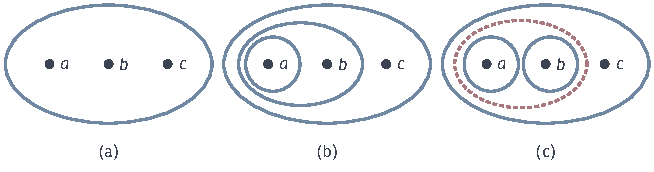
\includegraphics[width=110.786mm]{figures/04-spaces-measures-and-geometry/01-topology-and-metric/tikz/topo-finite-topologies/figure.pdf}
  \caption{三点集$X=\{a,b,c\}$上的三个子集族，每条蓝色闭曲线圈出族中的一个集合，空集未画出。(a)只有$X$，是拓扑。(b)$\{a\}$、$\{a,b\}$、$X$层层嵌套，是拓扑。(c)有$\{a\}$与$\{b\}$却缺少它们的并$\{a,b\}$（红色虚线），不是拓扑。}
  \label{fig:topo-finite-topologies}
\end{BookInlineFigure}

图(b)对应的族是
\[
 \mathcal T=\bigl\{\varnothing,\ \{a\},\ \{a,b\},\ X\bigr\}.
\]
它的成员依次包含，任取两个，并是较大的那个，交是较小的那个，结果都还在族中，所以$\mathcal T$是拓扑。图(c)的族含有$\{a\}$和$\{b\}$，它们的并$\{a,b\}$却不在族中，并封闭这一条不成立。

\paragraph{同一集合上的不同拓扑}
拓扑是附加在集合上的结构，同一个集合可以配上很不相同的拓扑。两个极端情形最能说明这一点。

\begin{example}[离散拓扑与平凡拓扑]
\label{ex:topo-discrete-indiscrete}
对任意集合$X$，全部子集组成的族$\mathcal P(X)$满足定义~\ref{def:topo-topology}，称为\term{离散拓扑}（discrete topology）。这时每个单点集$\{x\}$都是开集，$x$附近只有它自己。

另一端是$\{\varnothing,X\}$，它也满足三条规则，称为\term{平凡拓扑}（indiscrete topology）。这时唯一包含$x$的开集是整个$X$，空间中任何两点都无法用开集区分。

在两点集$X=\{a,b\}$上，$\{\varnothing,\{a\},X\}$也是拓扑。包含$b$的开集只有$X$，它也包含$a$；$a$却有一个不含$b$的开集$\{a\}$。在这个拓扑下，$a$总在$b$的每个开集里，反过来却不成立，“附近”这一关系可以不对称。
\end{example}

清单越长，可用来围住点的区域越多，点与点之间就越能区分。设$\mathcal T_1\subseteq\mathcal T_2$是同一集合上的两个拓扑，称$\mathcal T_2$比$\mathcal T_1$\term{更细}（finer），$\mathcal T_1$比$\mathcal T_2$更粗。

离散拓扑最细，平凡拓扑最粗，$\mathbb R$的通常拓扑介于二者之间。两个拓扑也可以互不包含：在$\{a,b\}$上，$\{\varnothing,\{a\},X\}$与$\{\varnothing,\{b\},X\}$就谈不上谁更细。

\subsection{拓扑基}
\label{sec:topo-basis}

实轴的开集可以形状复杂，例如$\bigcup_{n\geq1}(1/(n+1),1/n)$，但每个开集都是若干开区间的并：对开集$U$的每个点$x$取一个含于$U$的区间$(x-r_x,x+r_x)$，这些区间的并恰好是$U$。只要知道“开区间”这一小类集合，就能确定全部开集。

这与线性空间中用基表示向量相似：基向量通过线性组合得到所有向量，基本开集通过取并得到所有开集。类比到这里为止，因为取并没有系数，表示方式一般也不唯一，“基”的成员之间也不要求任何独立性。

\begin{definition}[拓扑基]
\label{def:topo-basis}
设$(X,\mathcal T)$是拓扑空间，$\mathcal B\subseteq\mathcal T$。若每个开集都能写成$\mathcal B$中若干成员的并，就称$\mathcal B$为$\mathcal T$的一个\term{拓扑基}（basis for a topology），$\mathcal B$的成员称为基本开集。
\end{definition}

空集是$\mathcal B$中零个成员的并，所以这一要求对空集自动成立。判断一个开集族是否为拓扑基时，逐点检验往往更方便：$\mathcal B\subseteq\mathcal T$是拓扑基，当且仅当对每个开集$U$和每个$x\in U$，都存在$B\in\mathcal B$使
\begin{equation}
 x\in B\subseteq U.
 \label{eq:topo-basis-pointwise}
\end{equation}

必要性是因为$x$属于表示$U$的某个成员。充分性是因为把这些$B$对$x\in U$取并，得到的集合含于$U$，又包含$U$的每个点，所以恰好等于$U$。图~\ref{fig:topo-basis-criterion}(a)画的就是这个判据：靠近边缘的点只是需要更小的基本开集。

\paragraph{由一族集合生成拓扑}
在欧氏空间里，我们往往先想到一类形状简单的集合，再希望用它们生成拓扑。这时需要判断：一族子集在什么条件下能作为某个拓扑的基。

\begin{theorem}[生成拓扑的基]
\label{thm:topo-basis-criterion}
设$X$是集合，$\mathcal B$是$X$的一族子集，满足
\begin{enumerate}
  \item $\mathcal B$的成员覆盖$X$，即每个$x\in X$都属于某个$B\in\mathcal B$；
  \item 若$x\in B_1\cap B_2$，$B_1,B_2\in\mathcal B$，则存在$B_3\in\mathcal B$使$x\in B_3\subseteq B_1\cap B_2$。
\end{enumerate}
令$\mathcal T$为$\mathcal B$中成员的所有并组成的族，则$\mathcal T$是$X$上的拓扑，$\mathcal B$是它的拓扑基。反过来，任何拓扑的拓扑基都满足这两条。
\end{theorem}
\begin{proof}
空集是零个成员的并，由条件1，$X$是全部成员的并，所以$\varnothing,X\in\mathcal T$。若干个“$\mathcal B$中成员的并”再取并，仍是$\mathcal B$中成员的并，所以$\mathcal T$对任意并封闭。

剩下验证两个集合的交。设$U=\bigcup_iB_i$，$V=\bigcup_jB'_j$，$x\in U\cap V$。则存在一对$i,j$使$x\in B_i\cap B'_j$，由条件2可取$B_x\in\mathcal B$，使
\[
 x\in B_x\subseteq B_i\cap B'_j\subseteq U\cap V.
\]
对$x\in U\cap V$取并，得到
\[
 U\cap V=\bigcup_{x\in U\cap V}B_x\in\mathcal T.
\]

反过来，设$\mathcal B$是拓扑$\mathcal T$的基。$X$是开集，必是$\mathcal B$中成员的并，条件1成立。$B_1\cap B_2$是开集，把判据\eqref{eq:topo-basis-pointwise}用于它，就得到条件2。
\end{proof}

条件2的作用可以从图~\ref{fig:topo-basis-criterion}(b)看出：两个基本开集的交不必本身是基本开集，但在交的每个点处都要放得下一个基本开集。

\begin{BookInlineFigure}
  \centering
  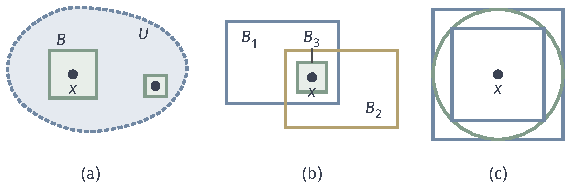
\includegraphics[width=96.227mm]{figures/04-spaces-measures-and-geometry/01-topology-and-metric/tikz/topo-basis-criterion/figure.pdf}
  \caption{拓扑基的三个判断。(a)开集$U$（虚线边界）中的每个点都有一个含于$U$的基本开集（绿色），靠近边界的点需要更小的方块。(b)定理条件2：在$B_1\cap B_2$的点$x$处放得下基本开集$B_3$。(c)以$x$为中心，正方形、圆盘、更小的正方形依次嵌套，所以方块与圆盘生成同样的开集。}
  \label{fig:topo-basis-criterion}
\end{BookInlineFigure}

条件2不能省略。在$X=\{a,b,c\}$上取$\mathcal B=\{\{a,b\},\{b,c\}\}$，它覆盖$X$。两个成员的交是$\{b\}$，而$\mathcal B$中没有成员能放进$\{b\}$，条件2不成立。所有的并组成的族是
\[
 \bigl\{\varnothing,\ \{a,b\},\ \{b,c\},\ X\bigr\},
\]
它不含$\{a,b\}\cap\{b,c\}=\{b\}$，的确不是拓扑。

\begin{example}[开区间与开矩形]
\label{ex:topo-intervals-rectangles}
全体开区间$(a,b)$构成$\mathbb R$通常拓扑的基，这正是本小节开头的观察。

在平面$\mathbb R^2$上，取全体开矩形$(a_1,b_1)\times(a_2,b_2)$组成的族$\mathcal B$。它覆盖$\mathbb R^2$，两个开矩形的交为
\[
\begin{aligned}
&\bigl((a_1,b_1)\times(a_2,b_2)\bigr)\cap\bigl((c_1,d_1)\times(c_2,d_2)\bigr)\\
&\qquad=\bigl((a_1,b_1)\cap(c_1,d_1)\bigr)\times\bigl((a_2,b_2)\cap(c_2,d_2)\bigr).
\end{aligned}
\]
两个开区间的交是开区间或空集，所以这个交仍是开矩形或空集，条件2成立。

由定理~\ref{thm:topo-basis-criterion}，开矩形生成$\mathbb R^2$上的一个拓扑，称为$\mathbb R^2$的通常拓扑。$\mathbb R^n$上用$n$个开区间的乘积同样处理。
\end{example}

不同的基可以生成同一个拓扑。在$\mathbb R^2$上改用全体开圆盘作基，条件1、2同样成立。如图~\ref{fig:topo-basis-criterion}(c)，圆盘内任一点周围都能放进一个以它为中心的小正方形，正方形内任一点周围也能放进一个小圆盘。由判据\eqref{eq:topo-basis-pointwise}，两族集合生成的开集完全相同，开集并不取决于用正方形还是圆形去度量附近。

\subsection{邻域}
\label{sec:topo-neighborhoods}

讨论一个点附近的性质时，用到的区域不必恰好是开集。要说“$f$在$x=1/2$附近取正值”，说它在$[0,1]$上取正值就够了，尽管$[0,1]$不是开集。关键在于这个集合包含一个围住$1/2$的开集。

\begin{definition}[邻域]
\label{def:topo-neighborhood}
设$X$是拓扑空间，$x\in X$。若集合$N\subseteq X$包含某个开集$U$，且$x\in U$，就称$N$是$x$的\term{邻域}（neighborhood）。本身是开集的邻域称为\term{开邻域}（open neighborhood）。
\end{definition}

在$\mathbb R$中，$[0,1]$是$1/2$的邻域，因为它包含开集$(1/4,3/4)\ni1/2$。它不是$0$的邻域，因为包含$0$的任何开集都含有负数，见图~\ref{fig:topo-neighborhoods}(a)。这说明两点：邻域本身不必是开集；“是邻域”总是相对于某个指定点而言，同一个集合可以是某些点的邻域而不是另一些点的邻域。

\begin{BookInlineFigure}
  \centering
  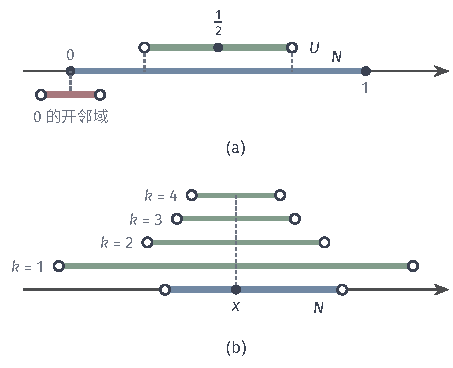
\includegraphics[width=76.793mm]{figures/04-spaces-measures-and-geometry/01-topology-and-metric/tikz/topo-neighborhoods/figure.pdf}
  \caption{邻域与邻域基。(a)蓝色的$N=[0,1]$包含绿色开集$U=(1/4,3/4)$，因此是$1/2$的邻域；$0$的任一开邻域（红色）都伸出$N$之外，所以$N$不是$0$的邻域。(b)绿色区间是$(x-1/k,x+1/k)$，蓝色区间是邻域$N=(x-0.4,x+0.6)$；$k=3$的区间已经含于$N$。}
  \label{fig:topo-neighborhoods}
\end{BookInlineFigure}

邻域与开集的关系可以反过来刻画开集：开集正是“对自己的每个点都是邻域”的集合。

\begin{lemma}[开集的邻域刻画]
\label{lem:topo-open-iff-neighborhood}
集合$U\subseteq X$是开集，当且仅当$U$是它的每个点的邻域。
\end{lemma}
\begin{proof}
若$U$开，对每个$x\in U$，$U$本身就是含$x$且含于$U$的开集。

反过来，若对每个$x\in U$都有开集$U_x$满足$x\in U_x\subseteq U$，则
\[
 U=\bigcup_{x\in U}U_x.
\]
拓扑对任意并封闭，所以$U$是开集。
\end{proof}

实轴开集的原始定义“每点两侧留有余地”正是这个引理的特例。以后证明一个集合是开集，常用的办法就是逐点找到含于其中的开邻域。

\subsection{邻域基}
\label{sec:topo-neighborhood-basis}

判断实数列$x_n\to x$时，并不需要检验$x$的所有邻域，只需检验区间$(x-1/k,x+1/k)$，$k=1,2,\dots$，因为任何邻域都包含其中某一个。这类足以代表所有邻域的子族，是描述一个点附近最经济的工具。

\begin{definition}[邻域基]
\label{def:topo-neighborhood-basis}
设$x\in X$，$\mathcal B_x$是$x$的一族邻域。若$x$的每个邻域$N$都包含$\mathcal B_x$中的某个成员，就称$\mathcal B_x$是$x$的\term{邻域基}（neighborhood basis）。
\end{definition}

在$\mathbb R$中，$\{(x-1/k,x+1/k):k\geq1\}$是$x$的邻域基。给定$x$的邻域$N$，它包含某个开集$U\ni x$，而$U$又包含某个$(x-r,x+r)$。取$k>1/r$，就有
\[
 \Bigl(x-\frac1k,x+\frac1k\Bigr)\subseteq(x-r,x+r)\subseteq N.
\]

图~\ref{fig:topo-neighborhoods}(b)是一个具体的情形：$N=(x-0.4,x+0.6)$的左侧余量是$0.4$，右侧余量是$0.6$，可取$r=0.4$。$k=2$时半径$0.5$超过左侧余量，$k=3$时半径$1/3<0.4$，区间已经含于$N$，更大的$k$也都一样。

闭区间族$\{[x-1/k,x+1/k]\}$同样是邻域基，所以邻域基的成员不必是开集。

\paragraph{邻域基与拓扑基的区别}
拓扑基与邻域基都是“用少数集合代表多数集合”，代表的对象却不同。拓扑基针对整个空间，用并生成每一个开集；邻域基只针对一个固定点，要求能塞进该点的每个邻域，并不生成任何开集。二者可以相互得到。

\begin{lemma}[由拓扑基得到邻域基]
\label{lem:topo-basis-to-neighborhood-basis}
若$\mathcal B$是$X$的拓扑基，则对每个$x\in X$，$\mathcal B_x=\{B\in\mathcal B:x\in B\}$是$x$的邻域基。反过来，若对每个$x$都选定一个由开集组成的邻域基$\mathcal B_x$，则$\bigcup_{x\in X}\mathcal B_x$是$X$的拓扑基。
\end{lemma}
\begin{proof}
设$N$是$x$的邻域，取开集$U$使$x\in U\subseteq N$。由判据\eqref{eq:topo-basis-pointwise}，有$B\in\mathcal B$使$x\in B\subseteq U$。这个$B$属于$\mathcal B_x$，且含于$N$。

反过来，设$U$开，$x\in U$。$U$是$x$的邻域，含有某个$B\in\mathcal B_x$，而$B$是开集且$x\in B$。于是$\bigcup_x\mathcal B_x$满足判据\eqref{eq:topo-basis-pointwise}。
\end{proof}

例如，$\mathbb R$的开区间基中包含$x$的那些区间构成$x$的邻域基，但它比$\{(x-1/k,x+1/k)\}$大得多：后者只用可数个集合就完成了同样的任务。一个点是否总有这样可数的邻域基，是第~\ref{sec:topo-countability}小节要讨论的问题。


\section{空间中的子集}
\label{sec:topo-subsets}

固定一个拓扑空间$X$，它的子集$A$与环境之间有几种自然的关系：$A$的补集是否开放，$A$中哪些点被$A$自身围住，环境中哪些点虽不在$A$内却紧贴着$A$。这些判断都相对于给定的拓扑，换一个拓扑，同一个集合的内部和闭包都可能改变。

\subsection{闭集}
\label{sec:topo-closed-sets}

开集描述“每点都留有余地”，与之互补的是“集合外每点都留有余地”：若$x\notin F$，则$x$有一个完全落在$F$外的开邻域。这正是说$X\setminus F$是开集。

\begin{definition}[闭集]
\label{def:topo-closed-set}
拓扑空间$X$的子集$F$称为\term{闭集}（closed set），如果它的补集$X\setminus F$是开集。
\end{definition}

De Morgan律把并变成交、把交变成并，于是定义~\ref{def:topo-topology}的三条规则转为闭集的三条规则：$\varnothing$与$X$是闭集；任意多个闭集的交是闭集；有限多个闭集的并是闭集。

“有限”同样不能去掉。在$\mathbb R$中，闭区间$[1/n,1]$（$n\geq1$）的并是
\[
 \bigcup_{n\geq1}\Bigl[\frac1n,1\Bigr]=(0,1],
\]
它不是闭集，因为补集$(-\infty,0]\cup(1,\infty)$在点$0$处没有落在其中的开邻域。

\paragraph{实轴上的区间}
闭区间$[a,b]$是闭集，因为补集$(-\infty,a)\cup(b,\infty)$是两个开集的并。开区间$(a,b)$不是闭集：补集$(-\infty,a]\cup[b,\infty)$含端点$a$，而$a$的每个开邻域都与$(a,b)$相交，所以补集不开。半开区间$[a,b)$既不是开集（$a$处没有余地），也不是闭集（补集在$b$处没有余地）。

\paragraph{开与闭不是互斥的两类}
日常语言里“开”与“闭”是反义词，在拓扑中它们却是两个独立的条件。$\mathbb R$本身和空集既开又闭，$[a,b)$既不开也不闭。离散拓扑中每个子集都既开又闭，平凡拓扑中只有$\varnothing$与$X$是闭集。

所以证明一个集合“不是开集”并不能推出它是闭集。既开又闭的子集在第~\ref{sec:topo-connected-sets}小节会成为判断空间能否拆分的工具。

\subsection{内部、闭包与边界}
\label{sec:topo-interior-closure}

一个子集$A$通常既不开也不闭，例如$[0,1)$。为了描述它离“开”和“闭”各差多少，我们按每一点与$A$的关系把空间中的点分类。图~\ref{fig:topo-interior-closure}画出了平面上的三种情形：有些点被$A$完全围住，有些点无论多小的邻域都同时碰到$A$与$A$的外部，还有些点有一个完全避开$A$的邻域。

\begin{BookInlineFigure}
  \centering
  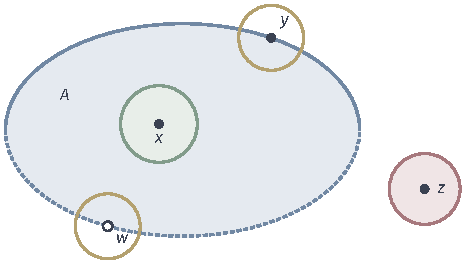
\includegraphics[width=78.807mm]{figures/04-spaces-measures-and-geometry/01-topology-and-metric/tikz/topo-interior-closure/figure.pdf}
  \caption{点与子集的三种关系。$A$是椭圆区域，实线部分的边界属于$A$，虚线部分不属于$A$。$x$有落在$A$内的邻域（绿色），是内点；$z$有与$A$不交的邻域（红色），不在闭包中；$y$与$w$的每个邻域（黄色）都既含$A$的点又含$A$外的点，二者都是边界点，其中$y\in A$，$w\notin A$。}
  \label{fig:topo-interior-closure}
\end{BookInlineFigure}

\paragraph{内部}
点$x$称为$A$的\term{内点}（interior point），如果$A$是$x$的邻域，即有开集$U$满足$x\in U\subseteq A$。$A$的全体内点组成$A$的\term{内部}（interior），记作$\operatorname{int}A$。

把每个内点的这种$U$合起来，得到$\operatorname{int}A$等于含于$A$的所有开集之并，因而它是含于$A$的最大开集。由引理~\ref{lem:topo-open-iff-neighborhood}，$A$开当且仅当$\operatorname{int}A=A$。

\paragraph{闭包}
从另一侧看，点$x$可能不在$A$中，却被$A$紧紧挨着：$x$的每个邻域都含有$A$的点。这时把$x$算作$A$能“接近”的点。

\begin{definition}[闭包]
\label{def:topo-closure}
设$A\subseteq X$。若$x$的每个邻域都与$A$相交，称$x$为$A$的\term{闭包点}（closure point）。$A$的全体闭包点组成的集合称为$A$的\term{闭包}（closure），记作$\overline A$。
\end{definition}

每个邻域都含一个开邻域，所以判断闭包点时只需检验开邻域，或者只需检验某个邻域基的成员。若$x\in A$，则$x$的每个邻域都含$x$，因而与$A$相交，所以$A\subseteq\overline A$。闭包也有一个与内部对称的刻画。

\begin{theorem}[闭包是最小闭超集]
\label{thm:topo-closure-smallest-closed}
对任意$A\subseteq X$，$\overline A$等于所有包含$A$的闭集之交。因此$\overline A$是闭集，并且是包含$A$的最小闭集；$A$闭当且仅当$\overline A=A$。
\end{theorem}
\begin{proof}
记$C$为包含$A$的所有闭集之交。若$x\notin\overline A$，则$x$有开邻域$U$与$A$不交。$X\setminus U$是包含$A$的闭集且不含$x$，所以$x\notin C$。这说明$C\subseteq\overline A$。

反过来，若$x\notin C$，则存在包含$A$的闭集$F$使$x\notin F$。$X\setminus F$是$x$的开邻域，它与$F$不交，因而与$A$不交，$x$不是闭包点。这说明$\overline A\subseteq C$。

闭集之交是闭集，所以$\overline A$闭。其余结论由“最小闭集”直接得到：$A$闭时$A$自己就是包含$A$的最小闭集。
\end{proof}

内部与闭包通过补集相互转换：$x$不是$A$的闭包点，恰好是说$x$有一个开邻域含于$X\setminus A$，即$x$是$X\setminus A$的内点。所以
\begin{equation}
 X\setminus\overline A=\operatorname{int}(X\setminus A).
 \label{eq:topo-closure-interior-complement}
\end{equation}

\paragraph{边界}
闭包与内部之差是那些既能接近$A$、又不被$A$围住的点。称
\begin{equation}
 \partial A=\overline A\setminus\operatorname{int}A
 \label{eq:topo-boundary}
\end{equation}
为$A$的\term{边界}（boundary）。由式~\eqref{eq:topo-closure-interior-complement}，$x\in\partial A$当且仅当$x$的每个邻域都既含$A$的点、又含$X\setminus A$的点。这个判据对$A$与$X\setminus A$对称，所以$\partial A=\partial(X\setminus A)$。

\begin{example}[同一集合在不同拓扑下]
\label{ex:topo-interior-closure-examples}
在$\mathbb R$的通常拓扑下取$A=[0,1)$。$(0,1)$中每点有含于$A$的小区间，$0$没有，所以$\operatorname{int}A=(0,1)$。$1$的每个邻域都含$A$中靠近$1$的点，$[0,1]$外的点有与$A$不交的邻域，所以$\overline A=[0,1]$。由式~\eqref{eq:topo-boundary}，$\partial A=\{0,1\}$。

有理数集$\mathbb Q$的内部为空，因为每个区间都含无理数。它的闭包是$\mathbb R$（见下一小节），所以$\partial\mathbb Q=\mathbb R$。

把$\mathbb R$换成离散拓扑，$A=[0,1)$既开又闭，于是
\[
 \operatorname{int}A=\overline A=A,\qquad\partial A=\varnothing.
\]

换成平凡拓扑，唯一含于$A$的开集是空集，唯一的非空开集$\mathbb R$与$A$相交，所以
\[
 \operatorname{int}A=\varnothing,\qquad\overline A=\mathbb R,\qquad\partial A=\mathbb R.
\]
\end{example}

表~\ref{tab:topo-three-topologies}把结果并排列出。同一个集合在三种拓扑下得到三组完全不同的答案，内部、闭包与边界描述的是集合在某个拓扑中的位置。

\begin{BookInlineTable}
  \centering
  \begin{tabular}{@{}llll@{}}
    \toprule
    $\mathbb R$上的拓扑 & $\operatorname{int}A$ & $\overline A$ & $\partial A$\\
    \midrule
    通常拓扑 & $(0,1)$ & $[0,1]$ & $\{0,1\}$\\
    离散拓扑 & $[0,1)$ & $[0,1)$ & $\varnothing$\\
    平凡拓扑 & $\varnothing$ & $\mathbb R$ & $\mathbb R$\\
    \bottomrule
  \end{tabular}
  \caption{集合$A=[0,1)$在三种拓扑下的内部、闭包与边界。}
  \label{tab:topo-three-topologies}
\end{BookInlineTable}

有限空间上可以完整地算一遍。取图~\ref{fig:topo-finite-topologies}(b)的拓扑，它的开集是$\varnothing,\{a\},\{a,b\},X$，取补集得到闭集
\[
 X,\quad\{b,c\},\quad\{c\},\quad\varnothing.
\]

设$A=\{b\}$。含于$A$的开集只有$\varnothing$，所以$\operatorname{int}A=\varnothing$。包含$A$的闭集是$\{b,c\}$与$X$，它们的交是$\{b,c\}$，由定理~\ref{thm:topo-closure-smallest-closed}得到
\[
 \overline A=\{b,c\},\qquad\partial A=\{b,c\}.
\]
点$c$也在闭包里，因为$c$唯一的开邻域$X$含有$b$。

在有距离的空间里，闭包点还能用“到$A$的距离为零”来刻画，这一判据依赖度量，放在第~\ref{chap:metric-spaces}章建立。

\subsection{稠密集}
\label{sec:topo-dense-sets}

每个实数都能被有理数任意接近，用闭包的语言，这就是说$\mathbb Q$的闭包是整个$\mathbb R$。把这一性质抽象出来，就是稠密。

\begin{definition}[稠密集]
\label{def:topo-dense}
若$D\subseteq X$满足$\overline D=X$，称$D$在$X$中\term{稠密}（dense）。
\end{definition}

由闭包的定义，$\overline D=X$意味着每个点的每个邻域都与$D$相交。每个非空开集都是它每个点的邻域，所以这又可以写成只涉及开集的判据。

\begin{theorem}[稠密的开集判据]
\label{thm:topo-dense-open-criterion}
$D$在$X$中稠密，当且仅当$X$的每个非空开集都与$D$相交。
\end{theorem}
\begin{proof}
设$D$稠密，$U$是非空开集，取$x\in U$。$U$是$x$的邻域，而$x\in\overline D$，所以$U\cap D\neq\varnothing$。

反过来，设每个非空开集都与$D$相交。任取$x\in X$及其邻域$N$，$N$含某个开集$U\ni x$。$U$非空，故与$D$相交，于是$N$也与$D$相交，$x\in\overline D$。
\end{proof}

\begin{example}[有理数与无理数都稠密]
\label{ex:topo-rationals-irrationals-dense}
由定理~\ref{thm:topo-dense-open-criterion}，只需证明每个开区间$(a,b)$（$a<b$）都含有理数和无理数。

由实数的Archimedes性质（由确界原理推出，可参考\BookChapterRef{chap:real-complex-functions}{卷一第4章“实数、复数与函数”}），可取正整数$n$使$1/n<b-a$，再取最小的整数$m$使$m/n>a$。由$m$的最小性，$(m-1)/n\leq a$，所以
\[
 a<\frac mn\leq a+\frac1n<b.
\]

用数字走一遍。设$(a,b)=(0.3,0.31)$，长度为$0.01$，取$n=101$。$30/101\approx0.2970$还小于$0.3$，所以$m=31$，得到
\[
 \frac{31}{101}\approx0.3069\in(0.3,0.31).
\]

对无理数，把同样的论证用于区间$(a-\sqrt2,b-\sqrt2)$，得到其中的有理数$q$，则$q+\sqrt2\in(a,b)$。$q+\sqrt2$是无理数，否则$\sqrt2=(q+\sqrt2)-q$会是有理数。所以$\mathbb Q$与$\mathbb R\setminus\mathbb Q$都在$\mathbb R$中稠密，而它们互不相交。
\end{example}

稠密并不要求子集占据大部分空间。$\mathbb Q$与无理数集都稠密，却彼此不交；第~\ref{chap:measure}章还会看到，$\mathbb Q$的长度为零。稠密只说明子集能接近空间中的每一点，并没有覆盖它们。

\paragraph{为什么不用点列定义稠密}
在$\mathbb R$中，$D$稠密等价于每个实数都是$D$中某个点列的极限。一般拓扑空间中，邻域可能多到无法用可数个依次缩小的集合代表，点列这时走不到闭包中的所有点。第~\ref{sec:topo-convergence}节将给出这样的空间，所以闭包与稠密性都以邻域定义，点列判据只在附加条件下成立。


\section{点列收敛}
\label{sec:topo-convergence}

实数列$x_n\to x$的定义是：对每个$\varepsilon>0$，存在$N$，使$n\geq N$时$\lvert x_n-x\rvert<\varepsilon$。条件$\lvert x_n-x\rvert<\varepsilon$就是$x_n\in(x-\varepsilon,x+\varepsilon)$，所以这句话等于说：对$x$的邻域基中每个区间，点列最终停在其中。把邻域基换成全部邻域，就得到不需要距离的收敛定义。

\begin{definition}[点列收敛]
\label{def:topo-sequence-convergence}
设$X$是拓扑空间，$(x_n)_{n\geq1}$是$X$中的点列，$x\in X$。若对$x$的每个邻域$N$，都存在$n_0$使$n\geq n_0$时$x_n\in N$，就称$(x_n)$\term{收敛}（converge）到$x$，记作$x_n\to x$，并称$x$为点列的一个\term{极限}（limit）。
\end{definition}

由于$x$的每个邻域都包含邻域基中的成员，只需对某个邻域基的成员检验这个条件。在$\mathbb R$上取邻域基$\{(x-\varepsilon,x+\varepsilon):\varepsilon>0\}$，定义~\ref{def:topo-sequence-convergence}就逐字回到实数列极限的$\varepsilon$-$N$定义，所以通常拓扑下的收敛与卷一的极限完全一致。

\paragraph{拓扑决定哪些点列收敛}
收敛完全由邻域决定，因此随拓扑而变。在离散拓扑中，$\{x\}$是$x$的邻域，$x_n\to x$意味着点列最终恒等于$x$。在平凡拓扑中，$x$的唯一邻域是整个空间，每个点列都收敛到每个点，极限可以不唯一。极限何时唯一，取决于不同点能否用不交的邻域分开，这是第~\ref{sec:topo-separation}小节的问题；在那之前，我们只说“一个极限”，而不说“极限”。

\paragraph{子列与闭集}
实数列的两条基本性质只用到邻域，因此在一般拓扑空间中照样成立：收敛点列的子列收敛到同一个点，闭集不会让其中点列的极限跑到集合外面。

\begin{theorem}[子列与闭包]
\label{thm:topo-subsequence-closure}
设$x_n\to x$。
\begin{enumerate}
  \item 对任意子列$(x_{n_k})$（$n_1<n_2<\cdots$），$x_{n_k}\to x$；
  \item 若所有$x_n$都属于集合$A$，则$x\in\overline A$；特别地，若$A$是闭集，则$x\in A$。
\end{enumerate}
\end{theorem}
\begin{proof}
对$x$的邻域$N$，取$n_0$使$n\geq n_0$时$x_n\in N$。由于$n_k\geq k$，当$k\geq n_0$时$n_k\geq n_0$，于是$x_{n_k}\in N$，第一条成立。

对第二条，$x$的每个邻域$N$都含有某个$x_n$，而$x_n\in A$，所以$N$与$A$相交，$x$是$A$的闭包点。$A$闭时$\overline A=A$。
\end{proof}

\paragraph{点列不能反推闭包}
在$\mathbb R$中，定理~\ref{thm:topo-subsequence-closure}的第二条可以反过来：$\overline A$中的每个点都是$A$中某个点列的极限，这是卷一闭集序列判据的内容。下面的例子说明，在一般拓扑空间中这个逆命题不成立，这也是第~\ref{sec:topo-dense-sets}小节不用点列定义稠密性的原因。

\begin{example}[余可数拓扑]
\label{ex:topo-cocountable}
在$\mathbb R$上规定：$U$为开集当且仅当$U=\varnothing$或$\mathbb R\setminus U$是可数集（有限或可数无限）。可数集的任意交、有限并仍可数，所以这些$U$对任意并和有限交封闭，构成一个拓扑，称为\term{余可数拓扑}（cocountable topology）。它的闭集是$\mathbb R$本身与全部可数集。

先看收敛的点列。设$x_n\to x$，令$C=\{x_n:x_n\neq x\}$，它是可数集，所以$\mathbb R\setminus C$是含$x$的开集。点列最终落在其中，即$n$充分大时$x_n\notin C$，也就是$x_n=x$。所以在这个拓扑中，只有最终恒定的点列才收敛。

再取$A=\mathbb R\setminus\{0\}$。包含$A$的闭集只能是$\mathbb R$，因为可数集不能包含不可数集$A$；于是$\overline A=\mathbb R\ni0$。但$A$中的点列若收敛，最终恒等于某个$A$中的点，极限不可能是$0$。所以$0\in\overline A$，却不是$A$中任何点列的极限。同时，$A$中收敛点列的极限都在$A$内，而$A$不是闭集：“包含点列的所有极限”在这里推不出闭性。
\end{example}

问题出在邻域的数量上。在$\mathbb R$的通常拓扑中，$0$的可数个邻域$(-1/k,1/k)$就能代表所有邻域，从每个中选一点即可造出趋于$0$的点列。余可数拓扑中$0$没有这样的可数邻域基：若$N_1,N_2,\dots$是$0$的邻域，各含开集$U_k\ni0$，则$\bigcup_k(\mathbb R\setminus U_k)$是可数个可数集之并，仍可数，于是可取$y\neq0$属于所有$U_k$；开集$\mathbb R\setminus\{y\}$是$0$的邻域，却不包含任何$N_k$。

第~\ref{sec:topo-countability}小节把“有可数邻域基”定义为第一可数性；在度量空间中这一条件自动成立，闭包与闭集的序列判据在第~\ref{chap:metric-spaces}章证明。


\section{连续映射}
\label{sec:topo-continuous-maps}

前两节研究一个空间内部的子集与点列，本节转向两个空间之间的映射。实函数$f$在$x_0$处连续的含义是：只要输入留在$x_0$附近某个足够小的区间内，输出就留在$f(x_0)$附近指定的区间内。这个要求可以改用开集表达，从而推广到任意拓扑空间。

\subsection{连续性的定义}
\label{sec:topo-continuity-definition}

先看$\varepsilon$-$\delta$定义在说什么。给定连续的$f:\mathbb R\to\mathbb R$及开集$V\subseteq\mathbb R$，设$f(x_0)\in V$，取$\varepsilon$使$(f(x_0)-\varepsilon,f(x_0)+\varepsilon)\subseteq V$。连续性给出$\delta>0$，使
\[
 (x_0-\delta,x_0+\delta)\subseteq f^{-1}(V).
\]
这对$f^{-1}(V)$的每个点成立，所以$f^{-1}(V)$是开集。逐点的“输入附近映入输出附近”就这样变成了一句关于原像的话。

图~\ref{fig:topo-preimage}(a)取$f(x)=x^2$，$V=(1,4)$，解$1<x^2<4$得
\[
 f^{-1}(V)=(-2,-1)\cup(1,2),
\]
这是开集。在点$x_0=3/2$处，$(1,2)$就是一个可用的区间，对应$\delta=1/2$。

图~\ref{fig:topo-preimage}(b)是有跳跃的函数，$x<1$时$f(x)=x$，$x\geq1$时$f(x)=x+1$。取$V=(3/2,5/2)$，$x<1$的部分取值小于$1$，不进入$V$；$x\geq1$的部分要求$x+1<5/2$。于是
\[
 f^{-1}(V)=[1,3/2),
\]
它含左端点而在那里没有余地，不是开集。跳跃恰好表现为某个开集的原像不开。

\begin{BookInlineFigure}
  \centering
  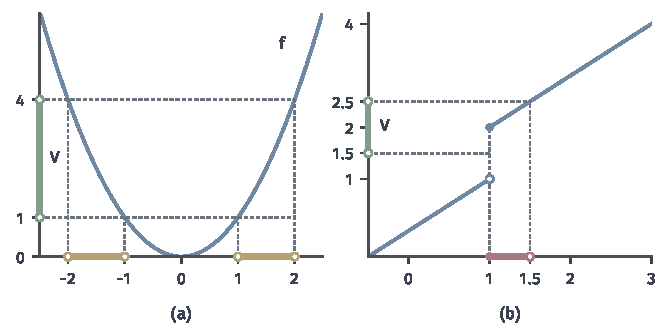
\includegraphics[width=112mm]{figures/04-spaces-measures-and-geometry/01-topology-and-metric/matplotlib/topo-preimage/figure.pdf}
  \caption{开集的原像。绿色是纵轴上的开区间$V$。(a)$f(x)=x^2$，$V=(1,4)$的原像是横轴上的$(-2,-1)\cup(1,2)$（黄色），仍是开集。(b)$f$在$x=1$处跳跃，$V=(3/2,5/2)$的原像是$[1,3/2)$（红色），含端点$1$，不是开集。}
  \label{fig:topo-preimage}
\end{BookInlineFigure}

\begin{definition}[连续映射]
\label{def:topo-continuous-map}
设$X,Y$是拓扑空间。映射$f:X\to Y$称为\term{连续映射}（continuous map），如果对$Y$的每个开集$V$，下面的原像都是$X$的开集：
\begin{equation}
 f^{-1}(V)=\{x\in X:f(x)\in V\}.
 \label{eq:topo-preimage}
\end{equation}
\end{definition}

定义用原像，是因为原像与集合运算相容：
\[
\begin{gathered}
 f^{-1}\Bigl(\bigcup_iV_i\Bigr)=\bigcup_if^{-1}(V_i),\qquad
 f^{-1}\Bigl(\bigcap_iV_i\Bigr)=\bigcap_if^{-1}(V_i),\\
 f^{-1}(Y\setminus V)=X\setminus f^{-1}(V).
\end{gathered}
\]
这些等式可参考\BookChapterRef{chap:sets-relations-maps}{卷一第1章“集合、关系与映射”}。由第一个等式，若$\mathcal B$是$Y$的拓扑基，只需检验每个$B\in\mathcal B$的原像为开集，因为任意开集都是基本开集之并。

\paragraph{等价判据}
定义~\ref{def:topo-continuous-map}是整体的说法。处理具体映射时，有时逐点检验更方便，有时检验闭集更方便。

\begin{theorem}[连续性的等价刻画]
\label{thm:topo-continuity-equivalent}
对映射$f:X\to Y$，下列条件等价：
\begin{enumerate}
  \item $f$连续；
  \item 对每个$x\in X$及$f(x)$的每个邻域$V$，存在$x$的邻域$U$使$f(U)\subseteq V$；
  \item 对$Y$的每个闭集$F$，$f^{-1}(F)$是$X$的闭集。
\end{enumerate}
\end{theorem}
\begin{proof}
1推出2。$V$含开集$V'\ni f(x)$，$U=f^{-1}(V')$是含$x$的开集，并且$f(U)\subseteq V'\subseteq V$。

2推出1。设$V$开，$x\in f^{-1}(V)$。$V$是$f(x)$的邻域，取$x$的邻域$U$使$f(U)\subseteq V$，则$U\subseteq f^{-1}(V)$。所以$f^{-1}(V)$是它每个点的邻域，由引理~\ref{lem:topo-open-iff-neighborhood}是开集。

1与3的等价来自等式$f^{-1}(Y\setminus F)=X\setminus f^{-1}(F)$：闭集的补集是开集，原像的补集是补集的原像。
\end{proof}

条件2在$X=Y=\mathbb R$时取邻域基$(x-\delta,x+\delta)$与$(f(x)-\varepsilon,f(x)+\varepsilon)$，就是$\varepsilon$-$\delta$定义，所以通常拓扑下的连续与卷一的连续一致。常值映射总是连续的，因为任何集合的原像只能是$\varnothing$或$X$。

\begin{example}[连续性依赖两边的拓扑]
\label{ex:topo-continuity-depends-topology}
考虑恒等映射$\operatorname{id}:\mathbb R\to\mathbb R$。若定义域取离散拓扑，则无论值域取什么拓扑，它都连续，因为定义域的每个子集都开。

若定义域取通常拓扑、值域取离散拓扑，则$\{0\}$在值域中开，原像$\{0\}$在定义域中不开，恒等映射不连续。同一个集合映射，连续与否由两边的开集族共同决定。
\end{example}

\paragraph{复合与点列}
连续映射的复合仍然连续。设$f:X\to Y$与$g:Y\to Z$连续，$W$是$Z$的开集，则
\[
 (g\circ f)^{-1}(W)=f^{-1}\bigl(g^{-1}(W)\bigr).
\]
先由$g$连续得到$g^{-1}(W)$开，再由$f$连续得到它的原像开。连续映射也保持已有的点列极限。

\begin{theorem}[连续映射保持极限]
\label{thm:topo-continuous-preserves-limits}
设$f:X\to Y$连续，$X$中的点列$x_n\to x$，则$f(x_n)\to f(x)$。
\end{theorem}
\begin{proof}
设$V$是$f(x)$的邻域。由定理~\ref{thm:topo-continuity-equivalent}，有$x$的邻域$U$使$f(U)\subseteq V$。由$x_n\to x$，$n$充分大时$x_n\in U$，于是$f(x_n)\in V$。
\end{proof}

反过来，“保持所有收敛点列的极限”能否推出连续，取决于点列能否探测定义域的拓扑。在余可数拓扑（例~\ref{ex:topo-cocountable}）中只有最终恒定的点列收敛，所以从这个空间出发的任何映射都保持极限。

然而从余可数拓扑的$\mathbb R$到通常拓扑的$\mathbb R$的恒等映射并不连续：开集$(0,1)$的补集不可数，原像$(0,1)$不是余可数拓扑的开集。在度量空间中，序列判据与连续性等价，这在第~\ref{chap:metric-space-maps}章证明。

\paragraph{原像与像}
连续性约束的是原像，对像没有直接约束。连续映射$f(x)=x^2$把开区间$(-1,1)$映成$[0,1)$，见图~\ref{fig:topo-image-openness}(a)，它不是开集。连续映射$g(x)=\arctan x$把闭集$\mathbb R$映成$(-\pi/2,\pi/2)$，它不是闭集。

像对集合运算的行为也不如原像整齐：像与并相容，但$f(A\cap B)$一般只包含于$f(A)\cap f(B)$。取$f(x)=x^2$，$A=\{-1\}$，$B=\{1\}$，则
\[
 f(A\cap B)=\varnothing,\qquad f(A)\cap f(B)=\{1\}.
\]

\subsection{开映射}
\label{sec:topo-open-maps}

上一小节的例子提出另一个问题：哪些映射把开集映成开集？这个条件与连续性平行，方向却相反。

\begin{definition}[开映射]
\label{def:topo-open-map}
映射$f:X\to Y$称为\term{开映射}（open map），如果对$X$的每个开集$U$，像$f(U)$是$Y$的开集。
\end{definition}

由于$f(\bigcup_iU_i)=\bigcup_if(U_i)$，验证开映射只需对定义域的某个拓扑基检验。

两个条件互不蕴含。常值映射$f(x)=c$连续，但$f((0,1))=\{c\}$不是开集，所以连续不保证开映射。反过来，从通常拓扑到离散拓扑的恒等映射（例~\ref{ex:topo-continuity-depends-topology}）把每个集合映成离散拓扑中的开集，是开映射，却不连续。

开映射的典型例子是平面到坐标轴的投影$p(x_1,x_2)=x_1$。开矩形$(a_1,b_1)\times(a_2,b_2)$的像是$(a_1,b_1)$，而开矩形构成拓扑基，所以$p$是开映射，见图~\ref{fig:topo-image-openness}(b)。

开映射也不必把闭集映成闭集。双曲线$\{(x_1,x_2):x_1x_2=1\}$是连续函数$x_1x_2$在闭集$\{1\}$上的原像，因而闭，它在$p$下的像却是$\mathbb R\setminus\{0\}$，见图~\ref{fig:topo-image-openness}(c)。这个像不含$0$，而$0$是它的闭包点，所以不闭。

\begin{BookInlineFigure}
  \centering
  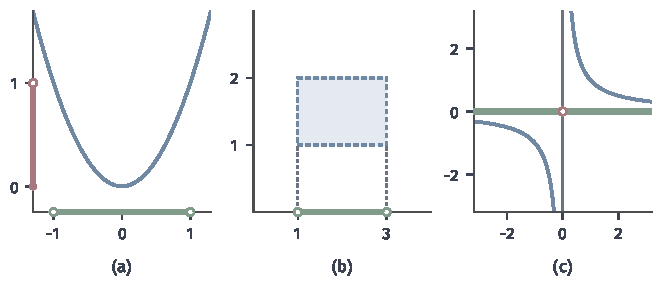
\includegraphics[width=112mm]{figures/04-spaces-measures-and-geometry/01-topology-and-metric/matplotlib/topo-image-openness/figure.pdf}
  \caption{像的开闭性。(a)$f(x)=x^2$把绿色开区间$(-1,1)$映成纵轴上的$[0,1)$（红色），连续而不开。(b)投影把开矩形$(1,3)\times(1,2)$映成开区间$(1,3)$。(c)闭集$x_1x_2=1$在投影下的像是绿色的$\mathbb R\setminus\{0\}$，缺少原点，不闭。}
  \label{fig:topo-image-openness}
\end{BookInlineFigure}

\subsection{同胚}
\label{sec:topo-homeomorphisms}

两个拓扑空间什么时候应当看作“相同”？线性代数中，可逆线性映射把一边的线性结构原样搬到另一边，于是两个同构的线性空间不必区分。拓扑中的对应角色是：一个双射把一边的开集恰好对应到另一边的开集。这时一切只用开集表述的概念（邻域、闭包、收敛、连续）都会被这个双射原样搬过去。

\begin{definition}[同胚]
\label{def:topo-homeomorphism}
双射$f:X\to Y$称为\term{同胚}（homeomorphism），如果$f$与逆映射$f^{-1}$都连续。存在同胚时，称$X$与$Y$同胚，记作$X\cong Y$。
\end{definition}

$f$连续说明$Y$的开集对应到$X$的开集。$f^{-1}$连续说明$X$的开集$U$的像$f(U)=(f^{-1})^{-1}(U)$是$Y$的开集。所以同胚在两边的开集族之间建立了一一对应，$x$的邻域也恰好对应到$f(x)$的邻域。

\begin{theorem}[连续双射成为同胚的条件]
\label{thm:topo-homeomorphism-open}
设$f:X\to Y$是连续双射。$f$是同胚，当且仅当$f$是开映射。
\end{theorem}
\begin{proof}
对$X$的开集$U$，$f$是双射，所以
\[
 (f^{-1})^{-1}(U)=\{y:f^{-1}(y)\in U\}=f(U).
\]
于是“$f^{-1}$连续”逐字等于“$f$把每个开集映成开集”。
\end{proof}

连续双射未必是同胚。例~\ref{ex:topo-continuity-depends-topology}中从离散拓扑到通常拓扑的恒等映射是连续双射，但不是开映射，因为$\{0\}$的像不开。第~\ref{sec:topo-subspaces}小节还会给出一个更直观的例子：把半开区间绕成圆周的映射。

\paragraph{同胚不保持长度}
同胚只要求开集对应，不要求保持距离、长度或有界性。仿射映射$x\mapsto a+(b-a)x$是$(0,1)$到$(a,b)$的同胚，它把长度伸缩了$b-a$倍。更进一步，映射
\begin{equation}
 h:(-1,1)\to\mathbb R,\qquad h(x)=\frac{x}{1-\lvert x\rvert}
 \label{eq:topo-interval-line-homeomorphism}
\end{equation}
把有界区间变成整条实轴。

它的逆映射是$h^{-1}(y)=y/(1+\lvert y\rvert)$。验证一下，设$y\geq0$，$x=y/(1+y)$，则$1-\lvert x\rvert=1/(1+y)$，于是
\[
 h(x)=\frac{y/(1+y)}{1/(1+y)}=y.
\]
$y<0$时由$h$是奇函数得到同样的结论。$h$与$h^{-1}$都由连续函数作除法得到，分母不为零，所以都连续。

在具体的点上，$h(1/2)=1$，$h(3/4)=3$，图~\ref{fig:topo-homeomorphism}(a)标出了这些点。输入越靠近$\pm1$，输出越大，距离被任意放大，开集的对应却没有被破坏。

\begin{BookInlineFigure}
  \centering
  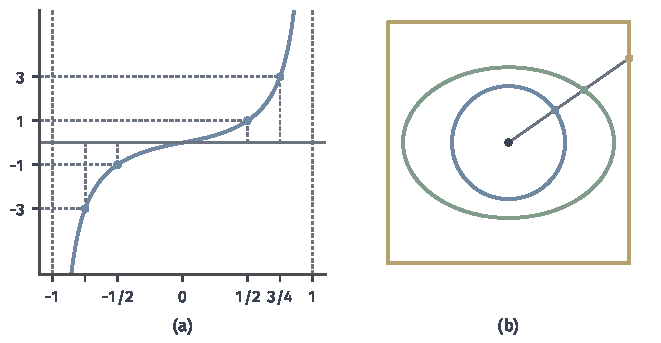
\includegraphics[width=112mm]{figures/04-spaces-measures-and-geometry/01-topology-and-metric/matplotlib/topo-homeomorphism/figure.pdf}
  \caption{同胚不保持度量性质。(a)$h(x)=x/(1-\lvert x\rvert)$把$(-1,1)$连续地拉成整条实轴，图中标出了$\pm1/2$与$\pm3/4$的函数值$\pm1$与$\pm3$。(b)从中心出发的射线与圆周、椭圆、正方形边界各交一点，沿射线移动这些交点就得到三条曲线之间的同胚。}
  \label{fig:topo-homeomorphism}
\end{BookInlineFigure}

有界性、长度都不是拓扑性质。拓扑性质指同胚保持的性质，例如本章后面的连通性与紧性。

同样，平面上的单位圆周与正方形边界同胚，这里的正方形边界是
\[
 \{\bm y:\max(\lvert y_1\rvert,\lvert y_2\rvert)=1\}.
\]
从原点出发的每条射线与两条曲线各交于一点，沿射线移动的映射是
\[
 F(\bm x)=\frac{\bm x}{\max(\lvert x_1\rvert,\lvert x_2\rvert)},\qquad
 F^{-1}(\bm y)=\frac{\bm y}{\sqrt{y_1^2+y_2^2}}.
\]

取$\bm x=(3/5,4/5)$，除以$4/5$得$F(\bm x)=(3/4,1)$；再除以其长度$5/4$，回到$(3/5,4/5)$。图~\ref{fig:topo-homeomorphism}(b)还画了椭圆，同样的射线也给出它与另外两条曲线的对应。三者周长和弯曲程度各不相同，拓扑只记录它们首尾相接成一圈的结构。要严格核对这类平面子集上的开集，需要下一节的子空间拓扑。


\section{空间的构造}
\label{sec:topo-constructions}

很多空间是从已有空间造出来的：圆周是平面的一部分，随时间运动的位置取值于“空间乘以时间”，圆周也可以由线段把两端粘合得到。这三种构造各有一个自然的映射，即包含映射、坐标投影和商映射。新空间的开集，就按“使这个映射连续”来规定，这条规则同时给出了判断映入或映出新空间的映射何时连续的方法。

\subsection{子空间}
\label{sec:topo-subspaces}

研究圆周$S^1=\{(x_1,x_2)\in\mathbb R^2:x_1^2+x_2^2=1\}$时，我们希望沿用平面的“附近”：圆周上一点附近，就是平面上这点附近与圆周的公共部分。

\begin{definition}[子空间拓扑]
\label{def:topo-subspace}
设$(X,\mathcal T)$是拓扑空间，$A\subseteq X$。下面的族是$A$上的拓扑，称为\term{子空间拓扑}（subspace topology）：
\begin{equation}
 \mathcal T_A=\{U\cap A:U\in\mathcal T\}.
 \label{eq:topo-subspace}
\end{equation}
称$(A,\mathcal T_A)$为$X$的子空间，$\mathcal T_A$的成员称为在$A$中\term{相对开}（relatively open）的集合。
\end{definition}

$\mathcal T_A$确实是拓扑：$\varnothing\cap A$与$X\cap A$分别给出$\varnothing$与$A$，并且
\[
 \bigcup_i(U_i\cap A)=\Bigl(\bigcup_iU_i\Bigr)\cap A,\qquad
 (U\cap A)\cap(V\cap A)=(U\cap V)\cap A.
\]

对补集取交同样可得：$A$中的相对闭集恰是形如$F\cap A$的集合，$F$为$X$的闭集。若$\mathcal B$是$X$的拓扑基，则$\{B\cap A:B\in\mathcal B\}$是子空间拓扑的基。

\paragraph{相对开与在环境中开}
相对开放比在环境中开放的要求低。取$X=\mathbb R$，$A=[0,1]$。如图~\ref{fig:topo-subspace-wrap}(a)，集合
\[
 [0,1/2)=(-1,1/2)\cap A
\]
在$A$中相对开，在$\mathbb R$中却不开。$A$本身作为子空间是全空间，因而在$A$中既开又闭，在$\mathbb R$中它只是闭集。

端点处的邻域只需单侧：$0$在$A$中的邻域基可以取$[0,1/k)$，$k\geq1$。单点集$\{0\}$在$A$中仍不开，因为每个相对开的含$0$集合都含有某个$[0,\varepsilon)$。

当$A$本身在$X$中开时，相对开集就是含于$A$的$X$的开集，因为两个开集的交仍开。上面的差别只出现在非开的子集上。描述子集的开闭性时，因此必须说明环境：“在$A$中开”与“在$X$中开”是两回事。

\paragraph{映入子空间的映射}
包含映射$\iota:A\to X$，$\iota(a)=a$，是连续的，因为$\iota^{-1}(U)=U\cap A$。子空间拓扑恰好使这一点成立：它是$A$上使$\iota$连续的最粗拓扑。因此，连续映射$f:X\to Y$限制到子空间上仍连续，因为$f|_A=f\circ\iota$。

\begin{lemma}[映入子空间的映射]
\label{lem:topo-map-into-subspace}
设$A\subseteq Y$为子空间，$g:Z\to A$。则$g$连续，当且仅当$\iota\circ g:Z\to Y$连续。
\end{lemma}
\begin{proof}
必要性是复合的连续性。充分性：$A$的每个开集形如$V\cap A$，$V$为$Y$的开集，而
\[
 g^{-1}(V\cap A)=(\iota\circ g)^{-1}(V)
\]
是开集。
\end{proof}

判断一个映入圆周的映射是否连续，只需把它看成映入平面的映射，逐坐标检验。例如$p(t)=(\cos2\pi t,\sin2\pi t)$作为$\mathbb R\to\mathbb R^2$连续（下一小节说明为什么可以逐坐标判断），因而作为$\mathbb R\to S^1$也连续。

\begin{example}[把半开区间绕成圆周]
\label{ex:topo-interval-to-circle}
限制$p$得到$p:[0,1)\to S^1$，其中$[0,1)$取$\mathbb R$的子空间拓扑。$p$是连续双射：圆周上的每个点恰对应$[0,1)$中的一个参数。但它不是同胚。

集合$[0,1/2)$在$[0,1)$中相对开，它的像是从$(1,0)$出发、沿逆时针走到$(-1,0)$之前的半圆弧，含端点$(1,0)$而不含$(-1,0)$。

这条弧在$S^1$中不是相对开的：$(1,0)$在$S^1$中的每个邻域都含有某个$p(t)$，其中$t$接近$1$，这些点位于$x_2<0$的一侧，不在弧上。所以$p$不是开映射，由定理~\ref{thm:topo-homeomorphism-open}，它不是同胚。
\end{example}

图~\ref{fig:topo-subspace-wrap}(b)显示了失败的原因：$[0,1)$在$0$处只有右侧的邻域，而圆周在$(1,0)$处两侧都有邻域。$p$把点一一对应，却没有对应它们的附近。

\begin{BookInlineFigure}
  \centering
  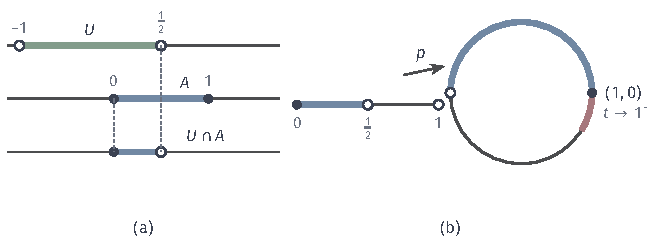
\includegraphics[width=111.774mm]{figures/04-spaces-measures-and-geometry/01-topology-and-metric/tikz/topo-subspace-wrap/figure.pdf}
  \caption{子空间中的相对开集。(a)绿色的$U=(-1,1/2)$在$\mathbb R$中开，与蓝色的$A=[0,1]$相交得到$[0,1/2)$，它在$A$中相对开，在$\mathbb R$中不开。(b)$p$把$[0,1/2)$（蓝色）绕成上半圆弧，弧含$(1,0)$；$(1,0)$下方的点（红色）来自$t$接近$1$的参数，不在弧上，所以弧不相对开。}
  \label{fig:topo-subspace-wrap}
\end{BookInlineFigure}

\subsection{有限乘积}
\label{sec:topo-finite-products}

描述平面上的位置需要两个实坐标，描述一个随时间变化的位置需要“空间中的点”与“时刻”两个分量。这类成对的数据取值于乘积集合$X\times Y$，我们需要在其上规定开集，使“两个分量都在各自的附近”成为乘积中的附近。

\begin{definition}[乘积拓扑]
\label{def:topo-product}
设$X,Y$是拓扑空间。下面的族生成的拓扑称为$X\times Y$上的\term{乘积拓扑}（product topology）：
\begin{equation}
 \mathcal B=\{U\times V:U\text{在}X\text{中开},\ V\text{在}Y\text{中开}\}.
 \label{eq:topo-product-basis}
\end{equation}
有限个空间$X_1\times\cdots\times X_n$的乘积拓扑同样由$U_1\times\cdots\times U_n$生成。
\end{definition}

$\mathcal B$满足定理~\ref{thm:topo-basis-criterion}的条件：$X\times Y$本身属于$\mathcal B$，并且
\[
 (U_1\times V_1)\cap(U_2\times V_2)=(U_1\cap U_2)\times(V_1\cap V_2)
\]
仍属于$\mathcal B$。

乘积拓扑的开集一般不是“开集乘开集”，而是这些开矩形的并，例如$\mathbb R^2$中的开圆盘。取$X=Y=\mathbb R$，这正是例~\ref{ex:topo-intervals-rectangles}中由开矩形生成的通常拓扑。若$X,Y$分别有拓扑基$\mathcal B_X,\mathcal B_Y$，则$\{B\times B':B\in\mathcal B_X,\ B'\in\mathcal B_Y\}$也是乘积拓扑的基。

\paragraph{投影与分量}
坐标投影$\pi_X(x,y)=x$与$\pi_Y(x,y)=y$是连续的：$\pi_X^{-1}(U)=U\times Y$是基本开集。它们也是开映射，因为基本开集$U\times V$（$V\neq\varnothing$）的像是开集$U$。

乘积拓扑是使两个投影都连续的最粗拓扑：若投影连续，$U\times Y$与$X\times V$必须开，它们的交$U\times V$也就必须开，图~\ref{fig:topo-product-neighborhood}(a)画的就是这个交。这一性质给出下面的判据。

\begin{theorem}[映入乘积的映射]
\label{thm:topo-map-into-product}
设$f:Z\to X\times Y$，写作$f(z)=(f_1(z),f_2(z))$，其中$f_1=\pi_X\circ f$，$f_2=\pi_Y\circ f$。则$f$连续，当且仅当$f_1$与$f_2$都连续。
\end{theorem}
\begin{proof}
若$f$连续，$f_1,f_2$是连续映射的复合，因而连续。

反过来，设$f_1,f_2$连续。对基本开集$U\times V$，有
\[
 f^{-1}(U\times V)=f_1^{-1}(U)\cap f_2^{-1}(V),
\]
这是两个开集的交，因而开。任意开集是基本开集之并，其原像是这些原像之并，所以$f$连续。
\end{proof}

由此，$\mathbb R^n$中的映射可以逐坐标判断连续性，上一小节的$p(t)=(\cos2\pi t,\sin2\pi t)$连续，正是因为两个分量都是连续实函数。这个判据只对映入乘积的映射成立。从乘积出发的映射，即使对每个分量单独连续，也未必整体连续：
\[
 f(x_1,x_2)=\frac{x_1x_2}{x_1^2+x_2^2}\quad(\text{原点处补定义为}0)
\]
在固定任一分量时对另一分量连续，沿对角线$x_1=x_2\neq0$却恒为$1/2$，所以在原点不连续。

\paragraph{空间与区间的乘积}
设$X$是拓扑空间，$I=[0,1]$取$\mathbb R$的子空间拓扑。乘积$X\times I$的点$(x,t)$可以理解为“时刻$t$时位于$x$”。一个连续映射$H:X\times I\to Y$同时记录了一族映射$H_t=H(\cdot,t):X\to Y$，$t\in I$。

乘积拓扑保证这族映射随$t$连续变化：如图~\ref{fig:topo-product-neighborhood}(b)，$(x,t)$的邻域含形如$U\times(t-\delta,t+\delta)$的基本开集（在$I$的端点处只取单侧），所以$x$附近、$t$附近的输入都映到$H(x,t)$附近。每个$H_t$连续，是因为它是$H$与连续映射$x\mapsto(x,t)$的复合。

\begin{BookInlineFigure}
  \centering
  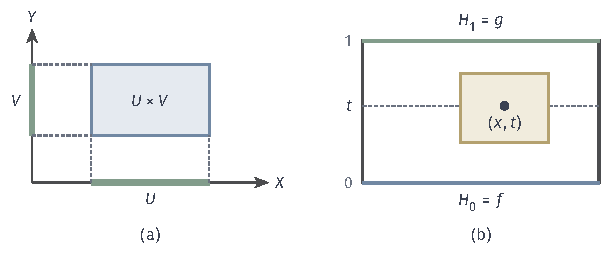
\includegraphics[width=102.404mm]{figures/04-spaces-measures-and-geometry/01-topology-and-metric/tikz/topo-product-neighborhood/figure.pdf}
  \caption{乘积拓扑的基本开集。(a)$U\times V$是投影下$U$与$V$的原像之交。(b)$X\times I$中$H_0=f$在底边，$H_1=g$在顶边，虚线是某一时刻的$H_t$；黄色方块是$(x,t)$的基本开邻域，同时限制空间位置与时刻。}
  \label{fig:topo-product-neighborhood}
\end{BookInlineFigure}

例如，对两个连续映射$f,g:X\to\mathbb R^n$，令
\[
 H(x,t)=(1-t)f(x)+tg(x).
\]
由定理~\ref{thm:topo-map-into-product}，$(x,t)\mapsto(f(x),g(x),t)$连续，$H$的每个坐标是这些分量经实数加法、乘法得到的，加法与乘法作为$\mathbb R^2\to\mathbb R$的映射连续，所以$H$连续。这时$H_0=f$，$H_1=g$，$H$把$f$逐渐变成$g$。

这种从一个映射连续变形到另一个映射的对象称为同伦，它是第~\ref{chap:homology}章的出发点，乘积$X\times I$正是它的定义域。

\subsection{商空间}
\label{sec:topo-quotients}

把一张纸条的两端粘起来，得到一个圈；把正方形的对边分别粘合，得到一个环面。这类构造把原空间中若干点看作同一点，然后问：粘合后的集合上，哪些子集应当算开集？

\paragraph{等价类与投影}
用等价关系$\sim$描述“看作同一点”：$x\sim y$表示$x$与$y$被识别。设$X/{\sim}$为全体等价类$[x]=\{y\in X:y\sim x\}$组成的集合，$q:X\to X/{\sim}$，$q(x)=[x]$，为把每点送到所在类的投影。我们希望$q$连续，而且在这一前提下尽可能多地保留开集。

\begin{definition}[商拓扑]
\label{def:topo-quotient}
设$X$是拓扑空间，$\sim$是$X$上的等价关系。规定$V\subseteq X/{\sim}$为开集，当且仅当$q^{-1}(V)$是$X$的开集。这样得到的拓扑称为\term{商拓扑}（quotient topology），$X/{\sim}$配上商拓扑称为\term{商空间}（quotient space），$q$称为\term{商映射}（quotient map）。
\end{definition}

原像与并、交相容，所以这个族满足拓扑的三条规则。按定义$q$连续，并且商拓扑是使$q$连续的最细拓扑：若$X/{\sim}$上的某个拓扑使$q$连续，它的每个开集$V$都满足$q^{-1}(V)$开，从而属于商拓扑。

子空间、乘积用“最粗”，商空间用“最细”，方向相反的原因在于新拓扑所在的一侧。包含映射与投影的新拓扑在定义域一侧，开集越多映射越容易连续，连续性只给出开集的下限，所以取满足下限的最粗者。商映射的新拓扑在值域一侧，开集越少映射越容易连续，连续性只给出开集的上限，所以取满足上限的最细者。

$q^{-1}(V)$是若干完整等价类之并，所以商空间的开集恰好对应$X$中由完整的类组成的开集。

\begin{example}[区间端点粘合成圆]
\label{ex:topo-interval-gluing-circle}
在$I=[0,1]$上令$0\sim1$，其余每点只与自身等价。等价类为$\{0,1\}$与单点集$\{t\}$（$0<t<1$）。

对内部的点$t$，它在商空间中的邻域就是$I$中$t$附近小区间的像。对粘合点$[0]=\{0,1\}$，集合$V$是它的开邻域，当且仅当$q^{-1}(V)$是含$0$与$1$的开集，因而包含某个$[0,\varepsilon)\cup(1-\varepsilon,1]$。

粘合点的邻域由区间两端的小段拼成，$[0]$两侧都有邻域，这正是例~\ref{ex:topo-interval-to-circle}中$[0,1)$缺少而圆周具有的结构。
\end{example}

取$\varepsilon=0.1$，用$p(t)=(\cos2\pi t,\sin2\pi t)$看，$[0,0.1)$绕出角度$[0^\circ,36^\circ)$，$(0.9,1]$绕出角度$(324^\circ,360^\circ]$。图~\ref{fig:topo-quotient-circle}中，两段在粘合点处接成一段连续的弧，这段弧恰好是圆周上$(1,0)$的开邻域。

\begin{BookInlineFigure}
  \centering
  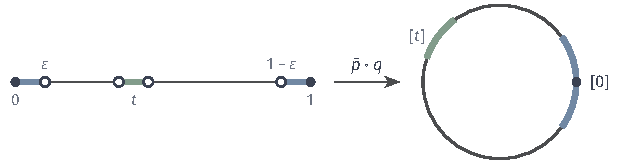
\includegraphics[width=105.11mm]{figures/04-spaces-measures-and-geometry/01-topology-and-metric/tikz/topo-quotient-circle/figure.pdf}
  \caption{区间端点粘合成圆，图中$\varepsilon=0.1$，$t=0.4$。蓝色的两段$[0,\varepsilon)$与$(1-\varepsilon,1]$在粘合后接成粘合点$[0]$的一段开邻域；绿色的小区间对应内部点$[t]$的开邻域。}
  \label{fig:topo-quotient-circle}
\end{BookInlineFigure}

\paragraph{从商空间出发的映射}
商空间上的映射通常是这样得到的：先在$X$上写出一个映射，再检验它在每个等价类上取同一个值。连续性则可以回到$X$上判断。

\begin{theorem}[商空间上的映射]
\label{thm:topo-quotient-maps}
设$q:X\to X/{\sim}$为商映射，$Z$为拓扑空间。
\begin{enumerate}
  \item 映射$g:X/{\sim}\to Z$连续，当且仅当$g\circ q:X\to Z$连续；
  \item 若$f:X\to Z$连续，并且$x\sim y$时$f(x)=f(y)$，则存在唯一的连续映射$\bar f:X/{\sim}\to Z$使$\bar f\circ q=f$。
\end{enumerate}
\end{theorem}
\begin{proof}
对$Z$的开集$W$，有
\[
 q^{-1}\bigl(g^{-1}(W)\bigr)=(g\circ q)^{-1}(W).
\]
按商拓扑的定义，$g^{-1}(W)$开当且仅当左边开，第一条成立。

对第二条，令$\bar f([x])=f(x)$。$f$在每个类上取同一个值，所以这个定义不依赖代表元的选择，并且$\bar f\circ q=f$。$q$是满射，满足这个等式的映射只能是$\bar f$。由$\bar f\circ q=f$连续及第一条，$\bar f$连续。
\end{proof}

把定理用于例~\ref{ex:topo-interval-gluing-circle}：$p:I\to S^1$连续且$p(0)=p(1)$，于是诱导出连续映射$\bar p:I/{\sim}\to S^1$。$p$在$(0,1)$上单射，并且只有$0,1$两点映到$(1,0)$，所以$\bar p$是双射。

到这里得到的只是连续双射。要说明$\bar p^{-1}$也连续，还需要关于紧性和分离性的工具，第~\ref{sec:topo-compact-images}小节完成这一步。另一方面，粘合可能破坏“不同点能用开集分开”这一性质，第~\ref{sec:topo-separation}小节会给出这样的商空间。


\section{空间的性质}
\label{sec:topo-properties}

前几节的例子显示，拓扑空间可以离日常的几何直觉很远：平凡拓扑中所有点都挤在一起，点列同时收敛到每个点；余可数拓扑中点列几乎探测不到闭包。本节集中研究整个空间满足的几类条件，它们排除这些病态现象，或者保证局部信息能够汇成整体信息。分离性问不同点能否被邻域分开；可数性与可分性问开集、邻域和稠密点集能否用可数个代表描述；连通性问空间能否拆成两块；紧性问开覆盖能否化为有限个。每项条件都用前面的点列、映射与构造来检验它的后果。

\subsection{分离性}
\label{sec:topo-separation}

在$\mathbb R$中，两个不同的点$x<y$可以分别放进$(x-r,x+r)$与$(y-r,y+r)$，其中$r=(y-x)/2$，两个区间不相交。平凡拓扑中做不到这一点，因为每个点的唯一开邻域都是全空间；正是这个缺陷让点列在平凡拓扑中有多个极限。

\begin{definition}[Hausdorff空间]
\label{def:topo-hausdorff}
若对$X$中任意两个不同的点$x\neq y$，都存在开集$U\ni x$与$V\ni y$使$U\cap V=\varnothing$，就称$X$为\term{Hausdorff空间}（Hausdorff space）。
\end{definition}

$\mathbb R$是Hausdorff空间。$\mathbb R^n$也是：若$\bm x\neq\bm y$，它们至少有一个坐标不同，设$x_i\neq y_i$，在第$i$个坐标上取两个不交的开区间，其余坐标取$\mathbb R$，得到两个不交的开矩形。这个论证对一般情形同样适用：两个Hausdorff空间的乘积仍是Hausdorff空间，因为两点在某个因子中不同，就在那个因子中分开。Hausdorff空间的子空间也是Hausdorff空间：若$U,V$在$X$中分开$x,y\in A$，则$U\cap A$与$V\cap A$在$A$中分开它们。所以平面上的圆周、曲线和区域都是Hausdorff空间。

\paragraph{极限的唯一性}
分离条件直接解决了第~\ref{sec:topo-convergence}节留下的极限唯一性问题。

\begin{theorem}[Hausdorff空间中极限唯一]
\label{thm:topo-hausdorff-unique-limit}
在Hausdorff空间中，每个收敛点列只有一个极限。
\end{theorem}
\begin{proof}
设$x_n\to x$且$x_n\to y$，$x\neq y$。取不交的开集$U\ni x$，$V\ni y$。存在$n_1$使$n\geq n_1$时$x_n\in U$，存在$n_2$使$n\geq n_2$时$x_n\in V$。取$n=\max\{n_1,n_2\}$，则$x_n\in U\cap V=\varnothing$，矛盾。
\end{proof}

因此在Hausdorff空间中可以写$\lim_{n\to\infty}x_n=x$。这个定理只需要两个邻域不交；它不要求空间有距离，也不需要可数性。

\paragraph{商空间是否仍可分离}
子空间与乘积保持Hausdorff性质，商空间则不一定，需要逐个检查。先看例~\ref{ex:topo-interval-gluing-circle}的商空间$I/{\sim}$（$0\sim1$）。两个内部点$[s]\neq[t]$（$0<s<t<1$）可以用$(0,1)$中两个不交小区间的像分开，这些像是开集，因为它们的原像就是这两个小区间。内部点$[t]$与粘合点$[0]$之间，取$\varepsilon<\min\{t,1-t\}/2$，用$(t-\varepsilon,t+\varepsilon)$的像与$[0,\varepsilon)\cup(1-\varepsilon,1]$的像分开；后者的原像正是这个并集，所以是开集。于是$I/{\sim}$是Hausdorff空间。

\begin{example}[有两个原点的直线]
\label{ex:topo-line-two-origins}
取两条实轴的并$X=\mathbb R\times\{0,1\}$（$\{0,1\}$取离散拓扑，$X$取乘积拓扑），对每个$t\neq0$令$(t,0)\sim(t,1)$，其余点只与自身等价。商空间$X/{\sim}$看起来像一条实轴，只是原点处有两个点$o_0=[(0,0)]$与$o_1=[(0,1)]$。

这两个原点不能被分开。设$V_0\ni o_0$、$V_1\ni o_1$是开集，则$q^{-1}(V_0)$是含$(0,0)$的开集，包含某个$(-\varepsilon,\varepsilon)\times\{0\}$；同样$q^{-1}(V_1)$包含某个$(-\varepsilon',\varepsilon')\times\{1\}$。取$0<t<\min\{\varepsilon,\varepsilon'\}$，则$[(t,0)]=[(t,1)]$同时属于$V_0$与$V_1$，所以二者相交。由此$X/{\sim}$不是Hausdorff空间，点列$[(1/n,0)]$同时收敛到$o_0$与$o_1$。
\end{example}

这个例子的每一点附近都像实轴的一段，局部看不出任何问题，整体却失去了极限唯一性。所以定义流形时，“局部像欧氏空间”之外还要单独要求Hausdorff条件，见第~\ref{chap:manifold-basics}章。

\subsection{可数性}
\label{sec:topo-countability}

$\mathbb R$有不可数个点，开集更多，但第~\ref{sec:topo-neighborhood-basis}小节已经看到，一个点的全部邻域可以由可数个区间$(x-1/k,x+1/k)$代表。类似地，全部开集能否由可数个基本开集生成？这两个问题分别针对一个点的邻域族和整个空间的开集族。

\begin{definition}[第一可数与第二可数]
\label{def:topo-countability}
若$X$的每个点都有一个可数的邻域基，称$X$\term{第一可数}（first countable）。若$X$有一个可数的拓扑基，称$X$\term{第二可数}（second countable）。
\end{definition}

这里“可数”包括有限。第一可数是逐点的条件，不同点的邻域基可以毫无关系；第二可数是整体的条件，要求一族可数的开集同时服务于所有点。由引理~\ref{lem:topo-basis-to-neighborhood-basis}，从可数拓扑基中取出含$x$的成员，就得到$x$的可数邻域基，所以第二可数蕴含第一可数。

\begin{example}[有理端点区间]
\label{ex:topo-rational-intervals}
在$\mathbb R$中，令$\mathcal B_{\mathbb Q}=\{(p,q):p,q\in\mathbb Q,\ p<q\}$。它是可数集，因为它与$\mathbb Q\times\mathbb Q$的一个子集一一对应，而可数集的有限乘积可数，可参考\BookChapterRef{chap:cardinality}{卷一第3章“基数”}。它是拓扑基：设$U$开，$x\in U$，取$r>0$使$(x-r,x+r)\subseteq U$，由$\mathbb Q$的稠密性取有理数$p\in(x-r,x)$与$q\in(x,x+r)$，则$x\in(p,q)\subseteq U$。

所以$\mathbb R$第二可数。同理，有理端点的开矩形$(p_1,q_1)\times\cdots\times(p_n,q_n)$构成$\mathbb R^n$的可数拓扑基：给定开集$U\ni\bm x$，先取开矩形$\bm x\in R\subseteq U$，再在每个坐标上把区间缩小为含$x_i$的有理端点区间。由于$\mathbb R^n$有不可数个点，这些例子说明，可数性条件约束的是开集族与邻域族的规模，而不是点的个数。
\end{example}

另一方面，第一可数不能推出第二可数。设$X$是不可数集，取离散拓扑。每个点有一个只含一个成员的邻域基$\{\{x\}\}$，所以$X$第一可数。但任何拓扑基$\mathcal B$都必须包含每个单点集：开集$\{x\}$是$\mathcal B$中成员的并，而这些成员都非空且含于$\{x\}$，只能是$\{x\}$本身。于是$\mathcal B$不可数，$X$不第二可数。

第一可数性的意义在于让点列重新可用：若$x\in\overline A$且$x$有可数邻域基$N_1\supseteq N_2\supseteq\cdots$（必要时取前$k$个的交），从每个$N_k\cap A$中选一点，得到的点列就收敛到$x$。例~\ref{ex:topo-cocountable}的余可数拓扑不第一可数，所以点列在那里失效。度量空间都是第一可数的，相应的闭包与闭集序列判据在第~\ref{chap:metric-spaces}章展开。第二可数性则是流形定义中的另一项要求，它保证流形可以由可数个坐标区域拼成。

\subsection{可分性}
\label{sec:topo-separability}

可数性条件谈的是开集族，另一种“可数描述”谈的是点：能否找到可数个点，使它们接近空间中的每一点？在$\mathbb R$中，可数的$\mathbb Q$就做到了这一点，因而数值计算只用有理数也能逼近任何实数。

\begin{definition}[可分空间]
\label{def:topo-separable}
若$X$含有一个可数的稠密子集，称$X$为\term{可分}（separable）空间。
\end{definition}

由例~\ref{ex:topo-rationals-irrationals-dense}，$\mathbb R$是可分的，尽管它不可数；$\mathbb R^n$也可分，$\mathbb Q^n$是可数稠密子集，因为每个非空开集含一个开矩形，开矩形的每个坐标区间都含有理数。可分性与可数性一样，并不限制点的个数。

\paragraph{可分性取决于拓扑}
同一个集合换一个拓扑，可分性可能改变。设$X$是不可数集，取离散拓扑。若$D$稠密，由定理~\ref{thm:topo-dense-open-criterion}，每个非空开集$\{x\}$都与$D$相交，即$x\in D$，所以唯一的稠密子集是$X$本身。$X$不可数，因此不可分。同一个$\mathbb R$，通常拓扑下可分，离散拓扑下不可分；而在平凡拓扑下，任何非空子集都稠密，单点集就够了。

\paragraph{三种可数要求的区别}
到这里出现了三种“可数”：可数稠密点集、可数拓扑基、每点的可数邻域基。它们分别描述点、整体开集族和逐点邻域族，不能互相替代。第二可数能推出可分：在可数拓扑基的每个非空成员中各选一点，得到可数集$D$；每个非空开集都含某个非空基本开集，因而与$D$相交，$D$稠密。

反过来，可分且第一可数的空间也未必第二可数。在$\mathbb R$上以全体半开区间$[a,b)$为基生成拓扑，称为\term{Sorgenfrey直线}（Sorgenfrey line）；两个半开区间的交仍是半开区间或空集，定理~\ref{thm:topo-basis-criterion}的条件成立。每个$[a,b)$都含有理数，所以$\mathbb Q$稠密，空间可分；$\{[x,x+1/k)\}$是$x$的可数邻域基，空间第一可数。但若$\mathcal B$是任意拓扑基，对每个$x$，开集$[x,x+1)$含$x$，必有$B_x\in\mathcal B$使$x\in B_x\subseteq[x,x+1)$，于是$x=\min B_x$。不同的$x$给出不同的$B_x$，所以$\mathcal B$不可数。

在度量空间中，第二可数与可分是等价的，这一结论在第~\ref{chap:metric-spaces}章证明；Sorgenfrey直线说明这个等价依赖距离，并非一般拓扑空间的性质。

\subsection{连通性}
\label{sec:topo-connectedness}

区间$[0,1]$是“一整块”，而$[0,1]\cup[2,3]$由两块组成。描述这种区别有两种思路：一是问空间能否被分成两个互不接触的部分，二是问任意两点能否用一条连续曲线连起来。前者只用开集，称为连通；后者需要显式的路径，称为路径连通。下面分别讨论，并说明在什么局部条件下二者一致。

\subsubsection{连通集}
\label{sec:topo-connected-sets}

$[0,1]\cup[2,3]$可以写成两个不交的非空集合之并，并且每一块都不包含另一块的闭包点，因而两块在这个空间中都是开集。连通就是排除这种分解。

\begin{definition}[连通空间]
\label{def:topo-connected}
若$X$不能写成两个不交的非空开集之并，称$X$\term{连通}（connected）。子集$A\subseteq X$称为连通集，如果$A$作为子空间连通。
\end{definition}

若$X=U\cup V$，$U,V$不交且开，则$U=X\setminus V$也是闭集。所以$X$连通，当且仅当$X$中既开又闭的子集只有$\varnothing$与$X$。这就是第~\ref{sec:topo-closed-sets}小节所说的用途：只要找到一个非平凡的既开又闭子集，空间就被拆开了。离散拓扑下超过一点的空间不连通，平凡拓扑下的空间总是连通的。

\paragraph{实轴上的连通集}
实轴上“没有缺口”的集合是区间：若$x,y\in A$且$x<z<y$，则$z\in A$。下面的定理说明，连通正好刻画了这一点。

\begin{theorem}[实轴上的连通集]
\label{thm:topo-connected-intervals}
子集$A\subseteq\mathbb R$连通，当且仅当$A$是区间。
\end{theorem}
\begin{proof}
若$A$不是区间，存在$x,y\in A$与$z\notin A$，$x<z<y$。则$A=((-\infty,z)\cap A)\cup((z,\infty)\cap A)$，两部分在$A$中相对开、不交，并分别含$x$与$y$，$A$不连通。

设$A$是区间，假设$A=U\cup V$，$U,V$在$A$中相对开、不交且非空。取$a\in U$，$b\in V$，不妨设$a<b$，则$[a,b]\subseteq A$。令$s=\sup(U\cap[a,b])$，则$s\in[a,b]\subseteq A$，下面说明$s$既不能在$U$中，也不能在$V$中。

若$s\in U$，则$s\neq b$，即$s<b$。$U$相对开，存在$\varepsilon>0$使$(s-\varepsilon,s+\varepsilon)\cap A\subseteq U$，于是$(s,\min\{s+\varepsilon,b\})$中的点属于$U\cap[a,b]$，且大于$s$，与上确界的定义矛盾。若$s\in V$，则$s\neq a$，即$s>a$，同样有$\varepsilon>0$使$(s-\varepsilon,s]\cap[a,b]\subseteq V$；这些点都不属于$U$，所以$U\cap[a,b]$中的点都不超过$s-\varepsilon$，与$s$是最小上界矛盾。
\end{proof}

所以$(0,1)$、$[0,1]$、$\mathbb R$都连通，而$(0,1)\cup(2,3)$不连通。证明中用到的是实数的确界原理，这正是“实轴没有缺口”的数学表述；在$\mathbb Q$中同样的论证失败，下文会看到$\mathbb Q$确实不连通。

\paragraph{连续像与介值}
连通性是只用开集表述的性质，连续映射通过原像把开集的分解拉回定义域，因此不能凭空制造分解。

\begin{theorem}[连通集的连续像]
\label{thm:topo-connected-image}
设$f:X\to Y$连续，$X$连通，则$f(X)$连通。
\end{theorem}
\begin{proof}
把$f$看成$X\to f(X)$的映射，由引理~\ref{lem:topo-map-into-subspace}它仍连续。若$f(X)=U\cup V$，$U,V$在$f(X)$中不交、开、非空，则$X=f^{-1}(U)\cup f^{-1}(V)$，两个原像开、不交，且因为$U,V$含有像点而非空，与$X$连通矛盾。
\end{proof}

与定理~\ref{thm:topo-connected-intervals}结合，就得到介值定理的一般形式：若$X$连通，$f:X\to\mathbb R$连续，则$f(X)$是区间；因此若$f$取到值$a<b$，它也取到$a,b$之间的每个值。特别地，同胚保持连通性，所以$[0,1)$与$(0,1)\cup(2,3)$不同胚。

\paragraph{连通分支}
不连通的空间可以分成若干“最大的连通块”。为此需要两个引理，说明连通集在什么情况下合并或扩大后仍连通。

\begin{lemma}[连通集的并与闭包]
\label{lem:topo-connected-union-closure}
\begin{enumerate}
  \item 若一族连通子集$A_i$（$i\in I$）有公共点$p$，则$\bigcup_iA_i$连通；
  \item 若$A$连通，且$A\subseteq B\subseteq\overline A$，则$B$连通。特别地，$\overline A$连通。
\end{enumerate}
\end{lemma}
\begin{proof}
记$S=\bigcup_iA_i$，设$S=U\cup V$，$U,V$在$S$中不交、相对开，不妨$p\in U$。对每个$i$，$A_i\cap U$与$A_i\cap V$在$A_i$中相对开、不交，并覆盖$A_i$；$A_i$连通且$p\in A_i\cap U$，所以$A_i\cap V=\varnothing$，即$A_i\subseteq U$。于是$S\subseteq U$，$V=\varnothing$，第一条成立。

对第二条，设$B=U\cup V$为$B$中不交、相对开的分解。同上，$A$连通，所以$A$整个落在其中一块，不妨$A\subseteq U$。若$V$非空，取$v\in V$，写$V=V'\cap B$，$V'$为$X$的开集。$V'$是$v$的邻域而$v\in\overline A$，所以$V'$与$A$相交；交点属于$A\cap V'\subseteq B\cap V'=V$，与$A\subseteq U$矛盾。故$V=\varnothing$。
\end{proof}

对$x\in X$，令$C(x)$为所有含$x$的连通子集之并。由引理第一条，$C(x)$连通，并且它是含$x$的最大连通子集，称为$x$所在的\term{连通分支}（connected component）。若$C(x)$与$C(y)$相交，二者之并连通且含$x$，由最大性等于$C(x)$，同理等于$C(y)$；所以连通分支两两不交，构成$X$的一个划分。由引理第二条，$\overline{C(x)}$也是含$x$的连通集，故$\overline{C(x)}=C(x)$，连通分支总是闭集。

\begin{example}[连通分支]
\label{ex:topo-components}
$(0,1)\cup(2,3)$的连通分支是$(0,1)$与$(2,3)$。$\mathbb Q$的连通分支是全部单点集：若$A\subseteq\mathbb Q$含两个有理数$p<q$，取无理数$z\in(p,q)$，$(-\infty,z)\cap A$与$(z,\infty)\cap A$就把$A$分开。单点集在$\mathbb Q$中不是开集，所以连通分支一般只是闭集，不必是开集。
\end{example}

\subsubsection{路径连通性}
\label{sec:topo-path-connected}

连通性告诉我们空间不能被拆开，却没有给出从一点到另一点的具体方式。在平面区域中，我们更习惯用一条曲线把两点连起来。下面把“曲线”定义为区间的连续像。

\begin{definition}[路径与路径连通]
\label{def:topo-path-connected}
设$I=[0,1]$。连续映射$\gamma:I\to X$称为从$\gamma(0)$到$\gamma(1)$的\term{路径}（path）。若$X$中任意两点之间都有路径，称$X$\term{路径连通}（path-connected）。
\end{definition}

在$\mathbb R^n$中，线段$\gamma(t)=(1-t)\bm a+t\bm b$是从$\bm a$到$\bm b$的路径，由逐坐标判据它连续；所以$\mathbb R^n$本身、开矩形、开圆盘以及一切凸集都路径连通。

\paragraph{路径分支}
“$x$与$y$之间有路径”是$X$上的等价关系。自反性用常值路径；对称性用反向路径$\bar\gamma(t)=\gamma(1-t)$。传递性需要把从$x$到$y$的路径$\alpha$与从$y$到$z$的路径$\beta$接起来：
\begin{equation}
(\alpha\cdot\beta)(t)=
\begin{cases}
\alpha(2t), & 0\leq t\leq 1/2,\\
\beta(2t-1), & 1/2\leq t\leq 1.
\end{cases}
\label{eq:topo-path-concatenation}
\end{equation}
在$t=1/2$处两段都给出$y$，所以定义无歧义。它的连续性来自下面的粘接引理：若$X=F_1\cup F_2$，$F_1,F_2$闭，$f$在每个$F_j$上的限制连续，则$f$连续。证明只需看闭集$C$的原像：$f^{-1}(C)=(f|_{F_1})^{-1}(C)\cup(f|_{F_2})^{-1}(C)$，每一部分在$F_j$中相对闭，因而形如$F_j$与闭集之交，在$X$中闭。

这个等价关系的等价类称为\term{路径分支}（path component）。路径连通的空间只有一个路径分支。

\paragraph{路径连通蕴含连通}
路径的像是区间$I$的连续像，由定理~\ref{thm:topo-connected-intervals}与定理~\ref{thm:topo-connected-image}是连通集。因此路径连通的空间一定连通：固定$x_0\in X$，对每个$y$取一条从$x_0$到$y$的路径$\gamma_y$，则$X=\bigcup_y\gamma_y(I)$，这些连通集有公共点$x_0$，由引理~\ref{lem:topo-connected-union-closure}，$X$连通。同理，每个路径分支都含于某个连通分支。

\begin{example}[连通但不路径连通]
\label{ex:topo-topologist-sine}
在$\mathbb R^2$中令$G=\{(x,\sin(1/x)):0<x\leq1\}$，$J=\{0\}\times[-1,1]$，$S=G\cup J$。$G$是区间$(0,1]$在连续映射$x\mapsto(x,\sin(1/x))$下的像，因而连通。对$(0,y)\in J$，取$\theta$使$\sin\theta=y$，则$x_k=1/(\theta+2k\pi)\to0$（$k$充分大时$x_k\in(0,1]$），而$(x_k,y)\in G$收敛到$(0,y)$，由定理~\ref{thm:topo-subsequence-closure}，$J\subseteq\overline G$。于是$G\subseteq S\subseteq\overline G$，由引理~\ref{lem:topo-connected-union-closure}，$S$连通。

但没有路径从$(0,0)$连到$(1,\sin1)$。假设$\gamma=(\gamma_1,\gamma_2):I\to S$是这样的路径。$T=\gamma_1^{-1}(\{0\})$是闭集，含$0$而不含$1$，令$t_0=\max T<1$。当$t>t_0$时$\gamma(t)\in G$，所以$\gamma_2(t)=\sin(1/\gamma_1(t))$。由$\gamma_2$在$t_0$处连续，取$\delta\in(0,1-t_0]$使$t\in[t_0,t_0+\delta]$时$\lvert\gamma_2(t)-\gamma_2(t_0)\rvert<1/2$。

记$a=\gamma_1(t_0+\delta)>0$。$\gamma_1$在$[t_0,t_0+\delta]$上从$0$连续变到$a$，由介值定理取遍$(0,a]$。取正整数$k$使$x^+=1/(\pi/2+2k\pi)$与$x^-=1/(3\pi/2+2k\pi)$都小于$a$，则有$t^\pm\in(t_0,t_0+\delta]$使$\gamma_1(t^\pm)=x^\pm$，相应地$\gamma_2(t^+)=1$，$\gamma_2(t^-)=-1$。这两个值相差$2$，却都与$\gamma_2(t_0)$相差小于$1/2$，矛盾。
\end{example}

集合$S$常称为拓扑学家的正弦曲线（topologist's sine curve）。它的问题出在$J$附近：$G$在$J$旁边无限次上下振荡，任何一个小邻域都把$S$切成无穷多段，路径无法在有限时间内穿过。排除这种局部现象，就能让连通与路径连通一致。

\paragraph{局部路径连通}
若对每个$x\in X$及$x$的每个邻域$N$，都存在路径连通的开集$V$使$x\in V\subseteq N$，称$X$\term{局部路径连通}（locally path-connected）。$\mathbb R^n$的开子集都局部路径连通：$\bm x$的邻域含一个以$\bm x$为中心的开矩形，开矩形是凸集，因而路径连通。

\begin{theorem}[局部路径连通时两种分支一致]
\label{thm:topo-locally-path-connected}
设$X$局部路径连通，则$X$的每个路径分支是开集，且路径分支与连通分支相同。特别地，连通且局部路径连通的空间是路径连通的。
\end{theorem}
\begin{proof}
设$P$是一个路径分支，$x\in P$。取路径连通的开集$V\ni x$，$V$中每点经$V$内的路径与$x$相连，所以$V\subseteq P$。于是$P$是开集。$X\setminus P$是其余路径分支之并，也是开集，所以$P$既开又闭。

设$C$是含$P$的连通分支（$P$连通，故含于一个连通分支）。$P\cap C=P$在$C$中既相对开又相对闭，且非空，由$C$连通得$P=C$。最后一句是$X$只有一个连通分支的情形。
\end{proof}

于是$\mathbb R^n$中连通的开集都是路径连通的，连通性可以用画出一条曲线来核验。例~\ref{ex:topo-topologist-sine}中的$S$在$J$上的点处不局部路径连通，定理的条件不满足。流形在每点附近同胚于欧氏空间的开集，因而局部路径连通，第~\ref{chap:manifold-basics}章将用这一点把流形的连通与路径连通等同起来。

\subsection{紧性}
\label{sec:topo-compactness}

闭区间上的连续函数有最大值，开区间上则未必；卷一把这一区别归结为闭区间的“有限子覆盖”性质。这个性质只用开集表述，因此可以搬到任何拓扑空间：它要求无论用什么方式以局部区域覆盖整个对象，都只需其中有限个。本小节先给出定义，再讨论闭包紧的集合，最后说明连续映射怎样保持紧性。

\subsubsection{紧性的定义}
\label{sec:topo-compact-definition}

一族开集$\{U_i\}_{i\in I}$若满足$\bigcup_iU_i=X$，称为$X$的\term{开覆盖}（open cover）；从中选出的、仍覆盖$X$的子族称为子覆盖，有限个成员组成的子覆盖称为\term{有限子覆盖}（finite subcover）。

\begin{definition}[紧空间与紧集]
\label{def:topo-compact}
若$X$的每个开覆盖都有有限子覆盖，称$X$\term{紧致}（compact），也称紧空间。子集$K\subseteq X$称为紧集，如果$K$作为子空间是紧的。
\end{definition}

子空间的开集是$U\cap K$的形式，所以$K$是紧集，当且仅当每一族满足$K\subseteq\bigcup_iU_i$的$X$的开集都有有限个成员仍覆盖$K$。以后检验紧集时直接用环境空间的开集，不必先转成相对开集。

\paragraph{某一个覆盖与所有覆盖}
定义中的量词是“每个开覆盖”。$(0,1)$有一个只含一个成员的开覆盖$\{(0,1)\}$，这不说明任何问题。考虑覆盖$\{(1/n,1):n\geq2\}$：每点$x\in(0,1)$在$n>1/x$时属于$(1/n,1)$，所以它覆盖$(0,1)$；但有限个成员之并是$(1/N,1)$，漏掉了$(0,1/N]$。所以$(0,1)$不紧。同理，$\{(-n,n):n\geq1\}$说明$\mathbb R$不紧。

闭区间$[a,b]$则是紧集，卷一已经用共同半径的论证证明了这一点。由下面的引理，$\mathbb R$中有界闭集都是紧集：它是某个$[a,b]$的闭子集。

\begin{lemma}[紧空间的闭子集]
\label{lem:topo-closed-in-compact}
紧空间$X$的闭子集$F$是紧集。
\end{lemma}
\begin{proof}
设$\{U_i\}$是$X$的开集，覆盖$F$。加上开集$X\setminus F$，得到$X$的开覆盖，取出有限子覆盖。去掉其中的$X\setminus F$（若出现），剩下的有限个$U_i$仍覆盖$F$。
\end{proof}

其他例子：有限集总是紧的，因为每点只需选一个含它的成员。无限集取离散拓扑时不紧，单点集组成的开覆盖没有有限子覆盖。平凡拓扑下的空间总是紧的，因为唯一的非空开集就是全空间。最后一例也说明，紧性本身不要求点能被分开。

在实轴上，紧性还可以用“每个点列有收敛子列”来刻画，卷一的证明正是在两种说法之间往返。一般拓扑空间中，两种说法可以不等价，点列也未必能探测拓扑，所以紧性以开覆盖定义。在度量空间中二者等价，并且紧等价于完备且全有界，这些判据在第~\ref{chap:metric-spaces}章建立。

\subsubsection{相对紧集}
\label{sec:topo-relatively-compact}

$(0,1)$本身不紧，但它离紧只差端点：补上闭包点后得到$[0,1]$，是紧集。很多估计只需要集合落在某个紧集里，而不需要集合本身紧，这引出下面的概念。

\begin{definition}[相对紧集]
\label{def:topo-relatively-compact}
设$A\subseteq X$。若$A$在$X$中的闭包$\overline A$是紧集，称$A$在$X$中\term{相对紧}（relatively compact）。
\end{definition}

$(0,1)$在$\mathbb R$中相对紧，但它既不闭也不紧；所以相对紧是比紧弱的条件。$\mathbb R$的每个有界子集都相对紧，因为它的闭包是有界闭集。紧集是否一定相对紧，涉及紧集的闭包；在Hausdorff空间中，这个问题由下面的引理回答。

\begin{lemma}[Hausdorff空间中的紧集是闭集]
\label{lem:topo-compact-closed-hausdorff}
设$X$是Hausdorff空间，$K\subseteq X$是紧集，则$K$是闭集。
\end{lemma}
\begin{proof}
取$x\notin K$。对每个$y\in K$，由Hausdorff条件取不交的开集$U_y\ni x$与$V_y\ni y$。$\{V_y\}_{y\in K}$覆盖$K$，取有限个$V_{y_1},\dots,V_{y_m}$覆盖$K$。则$U=U_{y_1}\cap\cdots\cap U_{y_m}$是含$x$的开集，与$V_{y_1}\cup\cdots\cup V_{y_m}\supseteq K$不交。所以$X\setminus K$是它每个点的邻域，是开集。
\end{proof}

由此，在Hausdorff空间中，紧集等于自己的闭包，因而相对紧；任何含于紧集$K$的子集$A$也相对紧，因为$\overline A$是$K$的闭子集，由引理~\ref{lem:topo-closed-in-compact}紧。没有Hausdorff条件时引理可以失效：平凡拓扑下超过一点的空间里，每个单点集都紧，却不闭。

\paragraph{相对紧依赖环境空间}
同一个集合在不同的环境中可能一个相对紧、一个不相对紧。把$(0,1)$看作空间$X=(0,1)$自身的子集，它在$X$中的闭包就是$X$，而$X$不紧，所以$(0,1)$在$(0,1)$中不相对紧；在$\mathbb R$中，它的闭包多了两个端点，成了紧集。这说明相对紧描述的是集合与环境的关系：环境中是否有足够的点让集合“收拢”。在度量空间中，相对紧可以用点列判据与全有界性来检验，这留到第~\ref{chap:metric-spaces}章。

\subsubsection{紧集的连续像}
\label{sec:topo-compact-images}

闭区间上连续函数取到最大值，这一结论的拓扑核心是：连续映射把紧集映成紧集，而实轴上的紧集有最大元。

\begin{theorem}[紧集的连续像]
\label{thm:topo-compact-image}
设$f:X\to Y$连续，$K\subseteq X$是紧集，则$f(K)$是$Y$中的紧集。
\end{theorem}
\begin{proof}
设$\{V_i\}$是$Y$的开集，覆盖$f(K)$。则$\{f^{-1}(V_i)\}$是$X$的开集，覆盖$K$：每个$x\in K$的像$f(x)$属于某个$V_i$。由$K$紧，取有限个$f^{-1}(V_{i_1}),\dots,f^{-1}(V_{i_m})$覆盖$K$，则$V_{i_1},\dots,V_{i_m}$覆盖$f(K)$。
\end{proof}

证明的方向值得注意：开覆盖在输出空间给出，经连续性拉回到输入空间，在那里用紧性有限化，再推回输出空间。连续性负责“拉回后仍是开覆盖”，紧性负责“有限化”，二者缺一不可。

\begin{theorem}[最大值与最小值]
\label{thm:topo-extreme-values}
设$K$是非空紧空间，$f:K\to\mathbb R$连续，则$f$有界，并且取到最大值与最小值。
\end{theorem}
\begin{proof}
由定理~\ref{thm:topo-compact-image}，$f(K)$是$\mathbb R$中的非空紧集。开区间$(-n,n)$（$n\geq1$）覆盖$f(K)$，有限个就够，所以$f(K)$含于某个$(-n,n)$，$f$有界。$\mathbb R$是Hausdorff空间，由引理~\ref{lem:topo-compact-closed-hausdorff}，$f(K)$是闭集。令$M=\sup f(K)$，对每个$\varepsilon>0$，$(M-\varepsilon,M+\varepsilon)$含$f(K)$中的点，所以$M\in\overline{f(K)}=f(K)$，即最大值$M$被取到。对$-f$用同样的论证得到最小值。
\end{proof}

两个条件都不能去掉。$f(x)=x$在$(0,1)$上连续，但$(0,1)$不紧，$f$没有最大值。在紧集$[0,1]$上，令$f(x)=x$（$x<1$）且$f(1)=0$，则$f$不连续，上确界$1$取不到。

\paragraph{同胚保持紧性}
若$h:X\to Y$是同胚，$X$紧，则$Y=h(X)$紧；反过来用$h^{-1}$。所以紧性与连通性一样是拓扑性质。由此，$[0,1]$与$(0,1)$不同胚，尽管二者都连通。紧性还给出判断同胚的一个有力工具，它回答了第~\ref{sec:topo-quotients}小节留下的问题。

\begin{theorem}[从紧空间到Hausdorff空间的连续双射]
\label{thm:topo-compact-hausdorff-homeomorphism}
设$X$紧，$Y$是Hausdorff空间，$f:X\to Y$是连续双射，则$f$是同胚。
\end{theorem}
\begin{proof}
只需证明$f^{-1}$连续，由定理~\ref{thm:topo-continuity-equivalent}，即证明$f$把$X$的闭集映成闭集，因为$(f^{-1})^{-1}(F)=f(F)$。设$F$在$X$中闭，由引理~\ref{lem:topo-closed-in-compact}，$F$紧；由定理~\ref{thm:topo-compact-image}，$f(F)$紧；由引理~\ref{lem:topo-compact-closed-hausdorff}，$f(F)$在$Y$中闭。
\end{proof}

现在回到例~\ref{ex:topo-interval-gluing-circle}。商空间$I/{\sim}=q(I)$是紧集$I$的连续像，因而紧；$S^1$是Hausdorff空间$\mathbb R^2$的子空间，因而是Hausdorff空间。所以连续双射$\bar p:I/{\sim}\to S^1$是同胚，“把线段两端粘起来”确实得到圆周。对照例~\ref{ex:topo-interval-to-circle}，$[0,1)\to S^1$同样是连续双射，却不是同胚；定理在那里不适用，因为$[0,1)$不紧。


\section{本章小结}
\label{sec:topo-summary}

章首问的是：没有距离时，怎样谈论“附近”“趋于”和“连续”。本章的回答是把开集族作为唯一的基本数据。实轴开集满足的三条规则（空集与全空间开，任意并开，有限交开）被取作拓扑的定义；拓扑基用并生成全部开集，邻域与邻域基则只描述一个点周围的区域。离散拓扑、平凡拓扑和余可数拓扑表明，同一集合上的不同拓扑会给出截然不同的“附近”。

在固定的拓扑下，子集与环境的关系由闭集、内部、闭包与边界描述，它们都由邻域判据定义，并随拓扑改变；稠密集是闭包为全空间的集合，等价于与每个非空开集相交。点列收敛要求点列最终落入极限的每个邻域，收敛点列的子列收敛到同一点，闭集留住已有的极限；但余可数拓扑的例子说明，一般空间中点列不能反推闭包，因此闭包与稠密性都不以点列定义。

映射的连续性由开集的原像为开集来定义，等价于逐点的邻域判据与闭集原像判据，并保持点列极限，反过来的序列判据需要额外条件。开映射约束的是像，与连续性互不蕴含；同胚是双向连续的双射，连续双射为同胚当且仅当它是开映射。$(-1,1)$与$\mathbb R$同胚表明，拓扑不记录长度和有界性。子空间、有限乘积与商空间分别使包含映射、坐标投影与商映射连续，并给出映入子空间与乘积、映出商空间的连续性判据；$X\times[0,1]$是同伦的定义域，区间端点的粘合给出圆周。

空间的性质中，Hausdorff条件保证极限唯一，子空间与乘积保持它，商空间则可能破坏它，有两个原点的直线就是例子。第二可数是整体开集族的可数性，第一可数是逐点邻域族的可数性，可分是可数稠密点集的存在性，三者都不限制点的个数；第二可数蕴含另外两者，Sorgenfrey直线说明反向一般不成立。连通性只用开集表述，实轴上的连通集恰为区间，连续像保持连通并推出介值定理；路径连通蕴含连通，拓扑学家的正弦曲线说明反向不成立，局部路径连通时两种分支一致。紧性要求每个开覆盖都可有限化，连续像保持紧性，由此得到最值定理；从紧空间到Hausdorff空间的连续双射是同胚，这证明了区间粘合确实得到圆周。

本章所有概念都不依赖距离，这也划定了它的边界。距离会带来更多结构：闭包可用点到集合的距离刻画，第二可数与可分等价，紧性可用序列紧与“完备且全有界”判断，这些是第~\ref{chap:metric-spaces}章的内容；连续性的距离判据、均匀连续与映射列的收敛在第~\ref{chap:metric-space-maps}章讨论。另一方面，连续变形保留什么信息，要借助本章的乘积与商构造，在第~\ref{chap:homology}章用同调来回答。


\chapter{度量空间}
\label{chap:metric-spaces}

用有理数$1.4,1.41,1.414,\ldots$逼近$\sqrt2$时，每一项都可以说清“误差小于$10^{-n}$”；用有限个格点代表一块平面区域时，也可以说清“每一点到最近格点的距离不超过$\varepsilon$”。第~\ref{chap:topological-spaces}章的拓扑能说一列点趋于某点、一个集合在另一个中稠密，却说不出这些定量的话：它只知道哪些集合是开的，不知道误差有多大。距离补上了这一层信息。有了距离，我们还能问拓扑问不出的问题：后项彼此越来越近的点列是否一定有极限，空间在给定精度下需要多少个代表。

本章先给出度量公理，用开球生成拓扑，说明此后的开集、邻域和收敛都可以用距离判断，并讨论距离带来的有界性与可分性判据；再说明怎样由已有的距离构造子空间、乘积空间以及零距离识别后的空间。随后两节把点列放在中心：收敛等价于距离趋零，闭包由点列极限刻画；只知道点列尾部相互接近时，完备性回答极限是否存在，并给出完备化与Baire纲定理。紧性的度量判据把开覆盖条件换成收敛子列，再拆成全有界与完备两部分。最后用覆盖数、打包数和度量熵计数有限精度下所需的代表。

本章只研究单个度量空间本身。连续映射的距离判据、均匀连续、映射列的收敛和压缩迭代在第~\ref{chap:metric-space-maps}章讨论；由向量空间结构和范数产生的度量在第~\ref{chap:normed-spaces}章系统展开；函数类的覆盖估计在第~\ref{chap:function-class-covers}章进行。

\section{度量}
\label{sec:metric-metrics}

平面上两点相距多远，答案取决于怎样走。直线飞行时用欧氏距离；只能沿东西、南北两个方向分别调整、并以较慢的一个方向为准时，用两个坐标差的最大值；只关心两个位置是否相同时，相同记为$0$，不同记为$1$。本节先比较这三种规则，提炼它们共同遵守的条件，得到度量的定义；再用开球把距离变成第~\ref{chap:topological-spaces}章的拓扑，并讨论距离额外提供的有界性与可分性判据。

\subsection{度量的定义}
\label{sec:metric-definition}

取平面上两点$\bm p=(0,0)$与$\bm q=(3,4)$。三种规则给出的距离分别是
\begin{equation*}
d_2(\bm p,\bm q)=\sqrt{3^2+4^2}=5,\qquad
d_\infty(\bm p,\bm q)=\max\{3,4\}=4,\qquad
d_0(\bm p,\bm q)=1,
\end{equation*}
其中$d_2(\bm x,\bm y)=\bigl((x_1-y_1)^2+(x_2-y_2)^2\bigr)^{1/2}$，$d_\infty(\bm x,\bm y)=\max\{\lvert x_1-y_1\rvert,\lvert x_2-y_2\rvert\}$，$d_0(\bm x,\bm y)$在$\bm x=\bm y$时为$0$、否则为$1$。三个数不同，判断“谁离$\bm p$近”的结果也不同：到$\bm p$的距离小于$1$的点，在$d_2$下组成圆盘，在$d_\infty$下组成边长为$2$的正方形，在$d_0$下只有$\bm p$本身。

数值不同，三种规则却有共同之处。每个距离都不小于零，并且只有两点相同时才为零；从$\bm p$到$\bm q$与从$\bm q$到$\bm p$的距离相同；绕经第三点不会比直接比较更近。把这三条作为公理，就得到不依赖坐标的距离概念。

\begin{definition}[度量]
\label{def:metric-metric}
设$X$是非空集合。映射$d:X\times X\to[0,\infty)$若对任意$x,y,z\in X$满足
\begin{enumerate}
\item 零距离判定：$d(x,y)=0$当且仅当$x=y$；
\item 对称性：$d(x,y)=d(y,x)$；
\item 三角不等式：$d(x,z)\leq d(x,y)+d(y,z)$，
\end{enumerate}
则称$d$为$X$上的一个\term{度量}（metric），称$(X,d)$为\term{度量空间}（metric space）。
\end{definition}

非负性已经写在取值范围$[0,\infty)$里。零距离判定保证距离能区分不同的点；对称性说明距离不带方向；三角不等式说明绕道不会缩短距离，它是后面几乎所有估计的来源。度量空间由集合与度量共同确定：同一个$\mathbb R^2$配上$d_2$、$d_\infty$或$d_0$，是三个不同的度量空间，下文提到“空间$X$”时总默认已经选定了度量。

三角不等式还有一个常用的变形。对任意$x,y,z$，由$d(x,z)\leq d(x,y)+d(y,z)$得$d(x,z)-d(y,z)\leq d(x,y)$，交换$x,y$的角色又得$d(y,z)-d(x,z)\leq d(x,y)$，所以
\begin{equation}
\lvert d(x,z)-d(y,z)\rvert\leq d(x,y).
\label{eq:metric-reverse-triangle}
\end{equation}
它说明：$x$移动多少，$x$到固定点$z$的距离至多变化多少。第~\ref{chap:metric-space-maps}章用它证明距离函数连续。

\begin{example}[三种平面距离的核对]
\label{ex:metric-three-metrics}
对$d_\infty$，前两条公理直接成立。三角不等式逐坐标核对：$\lvert x_i-z_i\rvert\leq\lvert x_i-y_i\rvert+\lvert y_i-z_i\rvert\leq d_\infty(\bm x,\bm y)+d_\infty(\bm y,\bm z)$对$i=1,2$都成立，再对$i$取最大值即可。对$d_0$，若$\bm x\neq\bm z$，则$\bm y$至少与其中一点不同，右端至少为$1$；若$\bm x=\bm z$，左端为$0$。欧氏距离$d_2(\bm x,\bm y)=\lVert\bm x-\bm y\rVert_2$的三角不等式就是欧氏范数的Minkowski不等式。更一般地，任意向量空间上的范数$\lVert\cdot\rVert$都给出度量$d(\bm x,\bm y)=\lVert\bm x-\bm y\rVert$；有限维情形的范数及其三角不等式可参考\BookChapterRef{chap:normed-inner-product-spaces}{卷二“赋范空间与内积空间”章}，一般赋范空间在第~\ref{chap:normed-spaces}章讨论。
\end{example}

度量的对象不必是数或向量。设$X=\{0,1\}^n$是长度为$n$的二进制串，$d_H(x,y)$记$x,y$取值不同的位置个数，称为\term{Hamming距离}（Hamming distance）。例如$d_H(0110,0011)=2$。若$x,z$在某个位置不同，则$y$在这个位置至少与$x,z$之一不同，所以$x,z$的每个不同位置都至少计入$d_H(x,y)$与$d_H(y,z)$中的一个，三角不等式成立。

并不是每个看起来合理的“差异量”都是度量。在$\mathbb R$上取$e(x,y)=(x-y)^2$，前两条公理成立，但$e(0,2)=4$，而$e(0,1)+e(1,2)=2$，三角不等式失败。平方误差放大了大的差异，经由中间点分两步走反而“更近”；这正是它不能直接当作距离使用的原因，而它的平方根$\lvert x-y\rvert$是度量。

\subsection{度量拓扑}
\label{sec:metric-topology}

有了距离，“$x$附近”最自然的含义是距离$x$小于某个正数的那些点。我们先给这类集合命名，再说明它们怎样生成第~\ref{chap:topological-spaces}章意义下的拓扑。

\begin{definition}[开球与闭球]
\label{def:metric-balls}
设$(X,d)$是度量空间，$x\in X$。对$r>0$，称
\begin{equation*}
B(x,r)=\{y\in X:d(x,y)<r\},\qquad B[x,r]=\{y\in X:d(x,y)\leq r\}
\end{equation*}
分别为以$x$为中心、$r$为半径的\term{开球}（open ball）与\term{闭球}（closed ball）。需要指明度量时写作$B_d(x,r)$。
\end{definition}

方括号提示闭球包含距离恰为$r$的点。闭球不一定是开球的闭包：在离散度量$d_0$下，$B(x,1)=\{x\}$，它的闭包仍是$\{x\}$，而$B[x,1]$是整个空间。所以本书不用$\overline{B(x,r)}$表示闭球。

开球的关键性质是：球内每一点都被一个更小的球包在球内。

\begin{lemma}[开球内的小球]
\label{lem:metric-ball-inside-ball}
若$y\in B(x,r)$，令$s=r-d(x,y)>0$，则$B(y,s)\subseteq B(x,r)$。
\end{lemma}

\begin{proof}
对$z\in B(y,s)$，由三角不等式，$d(x,z)\leq d(x,y)+d(y,z)<d(x,y)+s=r$，所以$z\in B(x,r)$。
\end{proof}

\begin{theorem}[开球构成拓扑基]
\label{thm:metric-balls-base}
度量空间$(X,d)$中全体开球构成$X$上某个拓扑的基。由这个基生成的拓扑中，$U\subseteq X$是开集当且仅当对每个$x\in U$都存在$r>0$使$B(x,r)\subseteq U$。
\end{theorem}

\begin{proof}
按第~\ref{chap:topological-spaces}章拓扑基的判定，要核对两件事。第一，每个$x$都属于开球$B(x,1)$，所以开球覆盖$X$。第二，设$z\in B(x_1,r_1)\cap B(x_2,r_2)$，由引理~\ref{lem:metric-ball-inside-ball}，取$s=\min\{r_1-d(x_1,z),r_2-d(x_2,z)\}>0$，则$B(z,s)$同时含于两个球，因而含于它们的交。

由基生成的开集是若干基元素的并。若$U$是开球之并，$x\in U$落在某个$B(y,t)\subseteq U$中，引理~\ref{lem:metric-ball-inside-ball}给出以$x$为中心、含于$B(y,t)$的球。反过来，若每个$x\in U$都有$B(x,r_x)\subseteq U$，则$U=\bigcup_{x\in U}B(x,r_x)$是开球之并。
\end{proof}

由开球生成的拓扑称为$d$的\term{度量拓扑}（metric topology）。今后说度量空间中的开集、闭集、邻域、收敛与连续，都指这个拓扑下第~\ref{chap:topological-spaces}章的概念。按定理~\ref{thm:metric-balls-base}，集合$N$是$x$的邻域当且仅当它包含某个开球$B(x,r)$；于是$B(x,1/n)$，$n=1,2,\ldots$，构成$x$的一个可数邻域基，因为任何$B(x,r)$都包含$n>1/r$时的$B(x,1/n)$。

\paragraph{点的分离}
距离为正的两点可以用半径为距离一半的球分开。设$x\neq y$，$r=d(x,y)/2>0$。若$z\in B(x,r)\cap B(y,r)$，则$d(x,y)\leq d(x,z)+d(z,y)<2r=d(x,y)$，矛盾，所以$B(x,r)$与$B(y,r)$不交。这说明度量拓扑满足Hausdorff条件：不同的点有不交的邻域。

这条性质给出一个限制：并非每个拓扑都来自某个度量。两点集$\{a,b\}$上的平凡拓扑只有$\varnothing$和全集两个开集，$a,b$无法用不交的开集分开，所以任何度量都不能诱导它。另一个直接推论是单点集是闭集：对$y\neq x$，球$B(y,d(x,y))$不含$x$，所以$X\setminus\{x\}$是开集。

\paragraph{用球判断子集的位置}
把第~\ref{chap:topological-spaces}章的定义换成球的语言，子集$A\subseteq X$与点$x$的关系可以这样判断：$x$是$A$的内点，当且仅当某个$B(x,r)\subseteq A$；$x$属于$A$的闭包，当且仅当每个$B(x,r)$都与$A$相交；$x$属于$A$的边界，当且仅当每个$B(x,r)$既与$A$相交、又与$X\setminus A$相交。这三条都由“开球构成邻域基”直接得到。

闭球是闭集。若$d(x,y)>r$，令$s=d(x,y)-r$，对$z\in B(y,s)$有$d(x,z)\geq d(x,y)-d(y,z)>r$，所以$B(y,s)$落在$B[x,r]$的补集中，补集是开集。

\begin{example}[开闭性与边界的判断]
\label{ex:metric-open-closed-interval}
在$\mathbb R$的通常度量$\lvert x-y\rvert$下考察$A=[0,1)$。点$0$的每个球都含有负数，所以$0$不是内点，$A$不是开集；点$1$的每个球都含有$A$中的点，$1$在闭包中却不在$A$中，所以$A$也不是闭集。按上面的判据，$A$的内部为$(0,1)$，闭包为$[0,1]$，边界为$\{0,1\}$。

换成离散度量$d_0$，每个单点集都是开球$B(x,1/2)$，于是任意子集都是开集，它的补集也是开集，所以任意子集同时是开集和闭集，边界总是空集。同一个集合$[0,1)$在两种度量下开闭性不同，再次说明开闭性取决于所选的度量。
\end{example}

不同的度量也可能给出相同的拓扑。在$\mathbb R^2$中，对任意$\bm x$和$r>0$，
\begin{equation*}
B_{d_\infty}(\bm x,r/\sqrt2)\subseteq B_{d_2}(\bm x,r)\subseteq B_{d_\infty}(\bm x,r),
\end{equation*}
这由$d_\infty\leq d_2\leq\sqrt2\,d_\infty$得到。于是一种度量下的每个球内都含有另一种度量下同心的球，按定理~\ref{thm:metric-balls-base}，两者的开集完全相同。离散度量$d_0$则给出不同的拓扑：单点集在$d_0$下是开集，在$d_2$下不是。什么时候两个度量“一样好”，取决于要保留开集、柯西列还是误差尺度，第~\ref{chap:metric-space-maps}章分别讨论。

\subsection{有界集}
\label{sec:metric-bounded}

拓扑只告诉我们哪些点“附近”，不告诉我们一个集合整体有多大。距离可以回答后一个问题：一个集合能否被某个有限半径的球装下。

\begin{definition}[有界集与直径]
\label{def:metric-bounded}
度量空间$(X,d)$的子集$A$若满足：存在$x\in X$和$r>0$使$A\subseteq B(x,r)$，则称$A$为\term{有界集}（bounded set）。非空集合$A$的\term{直径}（diameter）定义为$\operatorname{diam}A=\sup\{d(a,b):a,b\in A\}\in[0,\infty]$。空集规定为有界。
\end{definition}

球心的选取并不重要。若$A\subseteq B(x,r)$，对任意$y\in X$和$a\in A$，有$d(y,a)\leq d(y,x)+d(x,a)<d(y,x)+r$，所以$A\subseteq B(y,r+d(x,y))$：换一个球心，只需把半径加上两个球心的距离。同样的估计说明，非空集合有界当且仅当它的直径有限：若$A\subseteq B(x,r)$，则$d(a,b)\leq d(a,x)+d(x,b)<2r$；反过来，若$\operatorname{diam}A<\infty$，任取$a_0\in A$，就有$A\subseteq B(a_0,\operatorname{diam}A+1)$。

有界性与开闭性互不决定。在$\mathbb R$中，$(0,1)$有界且是开集；整数集$\mathbb Z$是闭集，因为它的补集是开区间之并，但它不能被任何有限半径的球容纳；$[0,1]$既有界又闭。可见判断一个集合“大小有限”，不能从它是否包含边界点来推断。

有界性还依赖于度量，而不只依赖于拓扑。在度量空间$(X,d)$上令$d'(x,y)=\min\{d(x,y),1\}$。前两条公理显然成立；对三角不等式，若$d(x,y)\geq1$或$d(y,z)\geq1$，右端至少为$1$，不小于左端；否则右端等于$d(x,y)+d(y,z)\geq d(x,z)\geq d'(x,z)$。半径小于$1$的球在$d$和$d'$下完全相同，所以两者拓扑相同，但在$d'$下每个集合都含于$B_{d'}(x,2)$，整个$\mathbb R$也成了有界集。

\subsection{可分性的判据}
\label{sec:metric-separability}

第~\ref{chap:topological-spaces}章区分了两种可数性：局部上，每个点有可数邻域基；整体上，整个空间有可数拓扑基。还定义了可分性：存在可数的稠密子集。在度量空间中，前一种总是成立，后两种恰好等价。

局部可数性已经在第~\ref{sec:metric-topology}小节得到：$\{B(x,1/n)\}_{n\geq1}$是$x$的邻域基。但这不能推出整个空间有可数拓扑基，因为每个点各自的可数个球合起来，在点数不可数时就不再可数。$\mathbb R$配上离散度量$d_0$就是例子：每个单点集$\{x\}=B(x,1/2)$都是开集，任何拓扑基必须为每个$x$提供一个含$x$且含于$\{x\}$的基元素，即$\{x\}$本身，所以拓扑基至少有不可数个元素。

\begin{theorem}[度量空间的可分性]
\label{thm:metric-separable-second-countable}
度量空间$(X,d)$可分，当且仅当它有可数拓扑基。
\end{theorem}

\begin{proof}
先设$D\subseteq X$可数且稠密。考虑族$\mathcal B=\{B(q,r):q\in D,\ r\in\mathbb Q,\ r>0\}$，它由两个可数集的乘积编号，所以可数。设$U$是开集，$x\in U$，取$r>0$使$B(x,r)\subseteq U$，再取有理数$s$满足$0<s<r/2$。由稠密性，开球$B(x,s)$含有某个$q\in D$。于是$x\in B(q,s)$，并且对$z\in B(q,s)$有$d(x,z)\leq d(x,q)+d(q,z)<2s<r$，即$B(q,s)\subseteq B(x,r)\subseteq U$。所以每个开集都是$\mathcal B$中元素之并，$\mathcal B$是拓扑基。

反过来，设$\{U_k\}_{k\geq1}$是可数拓扑基。对每个非空的$U_k$取一点$x_k\in U_k$，令$D$为这些点组成的集合，它可数。任意非空开集$V$是基元素之并，所以包含某个非空的$U_k$，从而含有$x_k\in D$。每个非空开集都与$D$相交，$D$稠密。
\end{proof}

证明的第一步用有理半径，是为了让球的总数可数；第二步只是从每个基元素中选一个代表点。在一般拓扑空间中，第二步仍然成立，即有可数基的空间可分；第一步却用到了距离和三角不等式，一般拓扑空间中可分不保证有可数基。

\begin{example}[欧氏空间的可数基]
\label{ex:metric-rn-separable}
在$(\mathbb R^n,d_2)$中，有理坐标点集$\mathbb Q^n$可数。给定$\bm x$和$\varepsilon>0$，逐个坐标取有理数$q_i$使$\lvert x_i-q_i\rvert<\varepsilon/\sqrt n$，则$d_2(\bm x,\bm q)<\varepsilon$，所以$\mathbb Q^n$稠密。按定理~\ref{thm:metric-separable-second-countable}，以有理坐标点为中心、有理数为半径的球构成可数拓扑基。前面的离散$\mathbb R$没有可数基，相应地它也不可分：每个单点集都是开集，稠密子集必须与每个单点集相交，只能是$\mathbb R$本身。
\end{example}

这个等价关系还有一个推论：可分度量空间的每个子集，按限制下来的度量也可分。原因是可数拓扑基$\{U_k\}$与子集$A$的交$\{U_k\cap A\}$构成$A$的可数拓扑基；这里用到子集上的拓扑恰是限制度量给出的拓扑，第~\ref{sec:metric-subspace}小节会证明这一点。例如$\mathbb R^2$中的任意曲线都可分，推论直接给出这一点，不需要具体找出它的可数稠密子集；对无理数集，也可以直接核对$\{q+\sqrt2:q\in\mathbb Q\}$是它的可数稠密子集。

\section{度量的构造}
\label{sec:metric-constructions}

第~\ref{chap:topological-spaces}章从已有空间构造了子空间、有限乘积和商空间，每次都规定了新空间的开集。有了距离以后，我们希望直接写出新空间的距离，并且让它诱导的拓扑恰好就是那里规定的拓扑。

本节逐项核对三种构造：把距离限制到子集，把各坐标的距离组合起来，以及先允许不同的点距离为零、再把这些点识别为一点。前两种对任意度量空间都可行；第三种只适用于由距离本身决定的识别，不能推广为任意商空间都有度量。

\subsection{子空间}
\label{sec:metric-subspace}

研究度量空间的一部分时，最直接的做法是保留原来的两点距离，只限制允许出现的点。

\begin{definition}[子空间度量]
\label{def:metric-subspace-metric}
设$(X,d)$是度量空间，$A\subseteq X$非空。限制$d_A=d|_{A\times A}$称为$A$上的\term{子空间度量}（subspace metric），$(A,d_A)$称为$X$的度量子空间。
\end{definition}

$A$中的点仍是$X$中的点，三条公理对$X$中任意点成立，自然对$A$中的点成立，所以$d_A$是度量。需要核对的是拓扑。$d_A$的开球是
\[
B_A(a,r)=\{y\in A:d(a,y)<r\}=B(a,r)\cap A,
\]
也就是环境中的球与$A$的交。

\begin{theorem}[子空间度量的拓扑]
\label{thm:metric-subspace-topology}
$d_A$诱导的拓扑等于$A$从$X$继承的子空间拓扑，即$V\subseteq A$在$(A,d_A)$中是开集，当且仅当存在$X$的开集$U$使$V=U\cap A$。
\end{theorem}

\begin{proof}
设$V$在$(A,d_A)$中是开集。对每个$a\in V$取$r_a>0$使$B_A(a,r_a)\subseteq V$，令$U=\bigcup_{a\in V}B(a,r_a)$。它是$X$的开集，并且
\[
U\cap A=\bigcup_{a\in V}\bigl(B(a,r_a)\cap A\bigr)=\bigcup_{a\in V}B_A(a,r_a)=V.
\]

反过来，设$U$是$X$的开集，$a\in U\cap A$。取$r>0$使$B(a,r)\subseteq U$，则$B_A(a,r)=B(a,r)\cap A\subseteq U\cap A$，所以$U\cap A$在$(A,d_A)$中是开集。
\end{proof}

于是第~\ref{chap:topological-spaces}章关于子空间的结论在度量子空间中都可以直接使用，只是开闭性要相对于$A$来判断。图~\ref{fig:metric-subspace-chord-arc}(a)是一个例子：在$\mathbb R$中取$A=[0,1]$，以$0$为中心、半径$1/2$的球在$A$中只剩$[0,1/2)$。

\begin{BookInlineFigure}
  \centering
  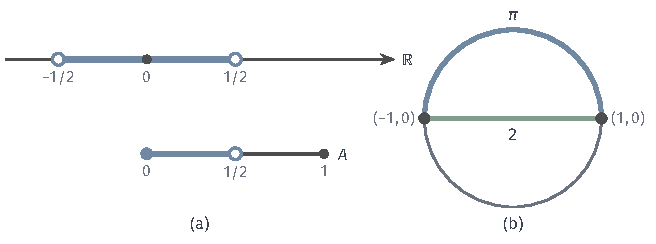
\includegraphics[width=111.1mm]{figures/04-spaces-measures-and-geometry/01-topology-and-metric/tikz/metric-subspace-chord-arc/figure.pdf}
  \caption{子空间的两个特点。(a)实轴上以$0$为中心、半径$1/2$的开球是$(-1/2,1/2)$，限制到$A=[0,1]$后成为$[0,1/2)$，它在$A$中是开集，在$\mathbb R$中不是。(b)单位圆周上，子空间度量量的是绿色弦长$2$，沿圆周的最短路径是蓝色半圆，长度$\pi$。}
  \label{fig:metric-subspace-chord-arc}
\end{BookInlineFigure}

这个集合可以写成$[0,1/2)=(-1/2,1/2)\cap A$，所以在$A$中是开集；$0$的左侧没有$A$的点，也就没有“越界”的点来破坏开性。再取$A=(0,1]$，它作为自身的子集总是闭集，但它在$\mathbb R$中不是闭集。环境决定了哪些点可以用来检验开闭。

子空间只保留环境中的两点距离，并不改用“沿着子集走”的距离。设$S^1=\{\bm x\in\mathbb R^2:\lVert\bm x\rVert_2=1\}$是单位圆周，如图~\ref{fig:metric-subspace-chord-arc}(b)所示，子空间度量下$(1,0)$与$(-1,0)$的距离是弦长$2$，而沿圆周走的最短长度是$\pi$。

弧长是圆周上另一个度量，它与弦长度量给出同样的拓扑，数值却不同。沿曲面或流形内部量出的路径长度需要切向量与长度的概念，在第~\ref{chap:riemannian-geometry}章建立。

\subsection{有限乘积空间}
\label{sec:metric-product}

几个度量空间的点组成坐标组时，需要一个距离同时比较各个坐标。设$(X_1,d_1),\ldots,(X_m,d_m)$是度量空间，$X=X_1\times\cdots\times X_m$，点记作$x=(x_1,\ldots,x_m)$。最常用的两种组合方式是求和与取最大：
\begin{equation}
\rho_1(x,y)=\sum_{i=1}^m d_i(x_i,y_i),\qquad
\rho_\infty(x,y)=\max_{1\leq i\leq m}d_i(x_i,y_i).
\label{eq:metric-product-metrics}
\end{equation}
这样定义的距离称为\term{乘积度量}（product metric）。$\mathbb R^2$上的$d_\infty$就是两个实轴的$\rho_\infty$。

两者都是度量。和或最大值为零，当且仅当每个$d_i(x_i,y_i)=0$，即每个坐标相同，这给出零距离判定；对称性逐坐标成立。三角不等式从每个坐标的不等式出发：
\[
d_i(x_i,z_i)\leq d_i(x_i,y_i)+d_i(y_i,z_i).
\]
对$\rho_1$，把这些不等式逐项相加。对$\rho_\infty$，右端两项分别不超过$\rho_\infty(x,y)$与$\rho_\infty(y,z)$，再对$i$取最大值。

两种度量还满足
\[
\rho_\infty\leq\rho_1\leq m\,\rho_\infty,
\]
因为$m$个非负数的和不小于其中最大的一个，也不超过最大者的$m$倍。图~\ref{fig:metric-ball-nesting}(b)画出了$m=2$时这组不等式对应的球的嵌套。与第~\ref{sec:metric-topology}小节的平面情形一样，它们的开球互相嵌套，诱导相同的拓扑。

\begin{theorem}[乘积度量的拓扑]
\label{thm:metric-product-topology}
$\rho_1$与$\rho_\infty$诱导的拓扑都等于第~\ref{chap:topological-spaces}章中$X_1,\ldots,X_m$的有限乘积拓扑。
\end{theorem}

\begin{proof}
由于两者诱导相同的拓扑，只需对$\rho_\infty$证明。乘积拓扑以形如$U_1\times\cdots\times U_m$（每个$U_i$是$X_i$的开集）的集合为基。最大值小于$r$等价于每个坐标距离都小于$r$，所以$\rho_\infty$的开球恰是
\[
B_{\rho_\infty}(x,r)=B_{d_1}(x_1,r)\times\cdots\times B_{d_m}(x_m,r).
\]
每个开球都是乘积拓扑的基元素，度量拓扑的开集都是乘积拓扑的开集。

反过来，设$x\in U_1\times\cdots\times U_m$。对每个$i$取$r_i>0$使$B_{d_i}(x_i,r_i)\subseteq U_i$，令$r=\min_i r_i$，则$B_{\rho_\infty}(x,r)\subseteq U_1\times\cdots\times U_m$。所以乘积拓扑的基元素在度量拓扑中也是开集。
\end{proof}

\begin{example}[两类坐标的乘积]
\label{ex:metric-product-two-coordinates}
取$X_1=\mathbb R$（通常距离）与$X_2=\{0,1\}^3$（Hamming距离），点$x=(0.2,010)$、$y=(0.5,011)$。实数坐标相差$0.3$，二进制串相差$1$位，于是
\[
\rho_1(x,y)=0.3+1=1.3,\qquad\rho_\infty(x,y)=\max\{0.3,1\}=1.
\]

在$\rho_\infty$下，$x$的半径$1/2$的球由第二坐标与$010$相同、第一坐标落在$(-0.3,0.7)$中的点组成：Hamming距离只取整数，要求它小于$1/2$就是要求两个串完全相同。
\end{example}

可见乘积距离小，意味着每个坐标都必须接近；哪个坐标先限制住球的形状，取决于各坐标距离的取值方式。

\subsection{伪度量}
\label{sec:metric-pseudometric}

有时我们只通过某些特征比较对象。比较平面上的点时如果只看横坐标，令
\begin{equation}
p(\bm x,\bm y)=\lvert x_1-y_1\rvert,
\label{eq:metric-first-coordinate-pseudometric}
\end{equation}
则$(0,0)$与$(0,5)$的“距离”为零，尽管它们是不同的点。$p$满足对称性和三角不等式，也满足$p(\bm x,\bm x)=0$，只缺零距离判定中“距离为零推出两点相同”这一半。

\begin{definition}[伪度量]
\label{def:metric-pseudometric}
设$X$非空。映射$p:X\times X\to[0,\infty)$若对任意$x,y,z\in X$满足$p(x,x)=0$、$p(x,y)=p(y,x)$与$p(x,z)\leq p(x,y)+p(y,z)$，则称$p$为$X$上的\term{伪度量}（pseudometric）。
\end{definition}

伪度量常由“忽略一部分信息”产生。向量空间上的\term{半范数}（seminorm）$\lVert\cdot\rVert$允许非零向量的长度为零，$p(\bm x,\bm y)=\lVert\bm x-\bm y\rVert$就是伪度量。第~\ref{chap:integration}章用积分比较函数时会遇到同样的情形：两个只在一个点上取值不同的函数，按积分算出的差异为零。

伪度量仍然有开球$B_p(x,r)=\{y:p(x,y)<r\}$。第~\ref{sec:metric-topology}小节证明开球构成拓扑基时，只用了“每点到自身距离为零”（使$x\in B(x,r)$）与三角不等式，没有用到“距离为零推出两点相同”。所以那里的论证逐字适用：伪度量的开球也生成一个拓扑，开集的球判据也相同。

这个拓扑不能区分零距离的点。在横坐标伪度量下，开球是一条竖直带形：
\[
B_p((0,0),1)=\{\bm x:\lvert x_1\rvert<1\},
\]
它同时包含$(0,0)$与$(0,5)$，见图~\ref{fig:metric-pseudometric-quotient}。一般地，若$p(x,y)=0$，则对任意$r>0$有$y\in B_p(x,r)$且$x\in B_p(y,r)$，于是$x$的每个开邻域都含有$y$，反之亦然。

所以只要存在不同的零距离点，伪度量拓扑就不满足Hausdorff条件。极限也随之不唯一：常值点列$(0,0),(0,0),\ldots$按$p$既趋于$(0,0)$，也趋于$(0,5)$。

\begin{BookInlineFigure}
  \centering
  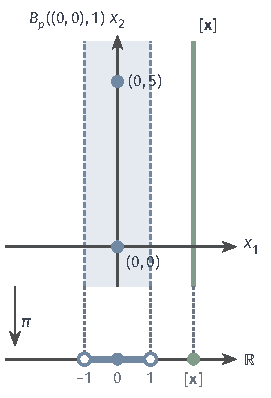
\includegraphics[width=45.903mm]{figures/04-spaces-measures-and-geometry/01-topology-and-metric/tikz/metric-pseudometric-quotient/figure.pdf}
  \caption{横坐标伪度量及其等价类。蓝色竖直带形是开球$B_p((0,0),1)$，点$(0,0)$与$(0,5)$同在其中，无法区分。绿色竖线是一个等价类$[\bm x]$。商映射$\pi$把每条竖线压成实轴上的一点，带形压成开区间$(-1,1)$。}
  \label{fig:metric-pseudometric-quotient}
\end{BookInlineFigure}

\subsection{零距离等价类上的度量}
\label{sec:metric-quotient}

既然伪度量无法区分零距离的点，自然的做法是把它们当成同一个点。下面验证这样做的每一步都合理，并说明得到的空间就是第~\ref{chap:topological-spaces}章意义下的商空间。

设$p$是$X$上的伪度量。规定$x\sim y$当且仅当$p(x,y)=0$。它是等价关系：自反性来自$p(x,x)=0$，对称性来自$p$的对称性，传递性来自
\[
p(x,z)\leq p(x,y)+p(y,z)=0.
\]
记$x$的等价类为$[x]$，商集为$X/{\sim}$，商映射为$\pi(x)=[x]$。

\begin{theorem}[零距离等价类上的度量]
\label{thm:metric-quotient-metric}
令$\hat d([x],[y])=p(x,y)$。则$\hat d$不依赖代表元的选取，是$X/{\sim}$上的度量，并且它诱导的拓扑等于$\pi$给出的商拓扑。
\end{theorem}

\begin{proof}
先证$\hat d$定义合理。设$x\sim x'$，$y\sim y'$。式~\eqref{eq:metric-reverse-triangle}的推导只用了对称性与三角不等式，所以对$p$也成立。于是
\[
\begin{aligned}
\lvert p(x,y)-p(x',y')\rvert
&\leq\lvert p(x,y)-p(x',y)\rvert+\lvert p(x',y)-p(x',y')\rvert\\
&\leq p(x,x')+p(y,y')=0.
\end{aligned}
\]

再核对公理。对称性与三角不等式从$p$继承。若$\hat d([x],[y])=0$，则$p(x,y)=0$，即$[x]=[y]$，零距离判定成立。

最后比较拓扑。由定义，$\pi$把$B_p(x,r)$映成$B_{\hat d}([x],r)$，并且
\[
\pi^{-1}\bigl(B_{\hat d}([x],r)\bigr)=B_p(x,r).
\]

设$V$在$\hat d$下是开集，$x\in\pi^{-1}(V)$。取$r$使$B_{\hat d}([x],r)\subseteq V$，则$B_p(x,r)\subseteq\pi^{-1}(V)$，所以$\pi^{-1}(V)$是$p$下的开集，$V$是商拓扑的开集。

反过来，设$\pi^{-1}(V)$是开集，$[x]\in V$。取$r$使$B_p(x,r)\subseteq\pi^{-1}(V)$，则$B_{\hat d}([x],r)=\pi(B_p(x,r))\subseteq V$，所以$V$在$\hat d$下是开集。
\end{proof}

回到横坐标伪度量。$(x_1,x_2)$的等价类是竖直线$\{x_1\}\times\mathbb R$，映射$[\bm x]\mapsto x_1$是$X/{\sim}$到$\mathbb R$的双射，并且
\[
\hat d([\bm x],[\bm y])=\lvert x_1-y_1\rvert.
\]
所以把零距离的点识别以后，得到的正是带通常距离的实轴：竖直方向的信息被丢掉，横坐标的距离被完整保留，这就是图~\ref{fig:metric-pseudometric-quotient}中从上到下的投影。

这一构造之所以可行，是因为等价关系由$p$自身给出，球在识别前后一一对应。对任意等价关系，商空间未必有度量。在$\mathbb R$上规定$x\approx y$当且仅当$x-y\in\mathbb Q$，考察商拓扑中的非空开集$U$。

$U$在$\mathbb R$中的原像是非空开集，含有某个区间$(a,b)$，又是若干等价类之并，因而含有$(a,b)+\mathbb Q=\mathbb R$。于是商拓扑只有空集和全集两个开集。商集有无穷多个点，两个不同的点不能用不交开集分开，按第~\ref{sec:metric-topology}小节的分离性，任何度量都不能诱导这个拓扑。

\section{点列收敛}
\label{sec:metric-convergence}

第~\ref{chap:topological-spaces}章用邻域定义收敛：$x_n\to x$是指$x$的每个邻域都包含点列中除有限项以外的全部项。这个定义要求逐个检查邻域，在度量空间中可以换成一个实数列的极限。

本节先证明这一点，再整理收敛点列的基本性质，并给出闭包、稠密与闭集的序列判据。序列判据的反向部分依赖“每点有可数个球作邻域基”，所以不能无条件搬到一般拓扑空间。

\begin{theorem}[收敛的距离判据]
\label{thm:metric-convergence-distance}
在度量空间$(X,d)$中，$x_n\to x$当且仅当实数列$d(x_n,x)\to0$。
\end{theorem}

\begin{proof}
设$x_n\to x$。对$\varepsilon>0$，$B(x,\varepsilon)$是$x$的邻域，所以存在$N$使$n\geq N$时$x_n\in B(x,\varepsilon)$，即$d(x_n,x)<\varepsilon$。

反过来，设$d(x_n,x)\to0$，$U$是$x$的邻域。按第~\ref{sec:metric-topology}小节，$U$包含某个$B(x,r)$。取$N$使$n\geq N$时$d(x_n,x)<r$，这些项就都落在$U$中。
\end{proof}

这个判据把点在空间中的运动压缩成一列实数。例如取平面点列
\[
x_n=\Bigl(\frac{\cos n}{n},\frac{\sin n}{n}\Bigr),
\]
它绕着原点$x$转圈，看上去方向杂乱，但到原点的距离恰为$d_2(x_n,x)=1/n$，由定理~\ref{thm:metric-convergence-distance}可知$x_n\to x$。

图~\ref{fig:metric-sequence-tail}把两种读法并排放在一起。取$\varepsilon=1/5$：不等式$1/n<1/5$等价于$n>5$，所以从第$N=6$项起，点列全部落进$B(x,\varepsilon)$。

\begin{BookInlineFigure}
  \centering
  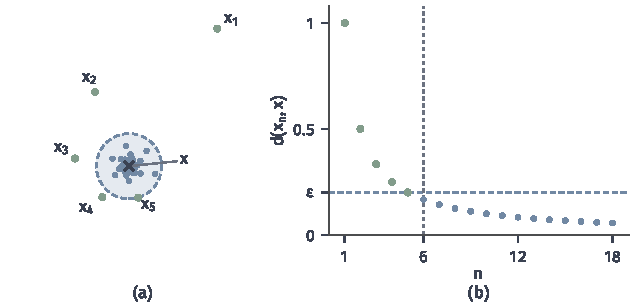
\includegraphics[width=108mm]{figures/04-spaces-measures-and-geometry/01-topology-and-metric/matplotlib/metric-sequence-tail/figure.pdf}
  \caption{点列$x_n=(\cos n/n,\sin n/n)$趋于原点$x$的两种读法，取$\varepsilon=1/5$。(a)平面上的点列，虚线圆是$B(x,\varepsilon)$，绿点是落在球外的前五项，蓝点是其后各项。(b)同一点列的距离数列$d(x_n,x)=1/n$，竖虚线处$N=6$，此后各点都在水平虚线$\varepsilon$之下。}
  \label{fig:metric-sequence-tail}
\end{BookInlineFigure}

判据的另外两个用法也值得记下。在乘积空间$(\mathbb R^m,\rho_\infty)$中，$\rho_\infty(\bm x_n,\bm x)\to0$当且仅当每个坐标的误差都趋于零，所以收敛就是逐坐标收敛；由于$\rho_1$与$\rho_\infty$诱导相同拓扑，换用$\rho_1$结论不变。

在离散度量$d_0$下，$d_0(x_n,x)$只取$0$和$1$，趋于零意味着从某项起恒为零。所以离散空间中的收敛点列，必须从某项起恒等于极限。

\subsection{收敛点列的性质}
\label{sec:metric-convergent-properties}

距离给出的第一个推论是极限唯一。若$x_n\to x$且$x_n\to y$，由三角不等式
\[
d(x,y)\leq d(x,x_n)+d(x_n,y)\to0,
\]
所以$d(x,y)=0$，由零距离判定得$x=y$。这里起作用的正是度量区分不同点的能力；第~\ref{sec:metric-pseudometric}小节的伪度量缺少这一条，常值点列可以同时趋于两个不同的点。

\begin{theorem}[收敛点列有界]
\label{thm:metric-convergent-bounded}
度量空间中的收敛点列，其全部项组成的集合是有界集。
\end{theorem}

\begin{proof}
设$x_n\to x$。取$N$使$n\geq N$时$d(x_n,x)<1$，前面只剩有限项，取它们的距离的最大值：
\[
r=1+\max\{d(x_1,x),\ldots,d(x_{N-1},x)\}
\]
（$N=1$时取$r=1$）。于是对每个$n$都有$d(x_n,x)<r$，全部项落在$B(x,r)$中。
\end{proof}

研究不收敛的点列时，常常从中挑出一部分。设$n_1<n_2<\cdots$是严格递增的正整数列，称$(x_{n_k})_{k\geq1}$为$(x_n)$的一个\term{子列}（subsequence）。严格递增保证$n_k\geq k$，所以$k\to\infty$时$n_k\to\infty$。

收敛点列的每个子列都收敛到同一个极限。设$x_n\to x$，对$\varepsilon>0$取$N$使$n\geq N$时$d(x_n,x)<\varepsilon$。当$k\geq N$时$n_k\geq N$，于是$d(x_{n_k},x)<\varepsilon$。

反方向不成立：一个点列有收敛的子列，不能推出它本身收敛。在$\mathbb R$中取$x_n=(-1)^n$，偶数项组成的子列恒为$1$，奇数项组成的子列恒为$-1$，各自收敛。若整列趋于某个$x$，两个子列都应趋于$x$，于是$x=1=-1$，矛盾。

整列收敛是比“存在收敛子列”强得多的要求，第~\ref{sec:metric-compactness}节的紧性判据只要求后者。

\subsection{闭包与闭集的序列判据}
\label{sec:metric-closure-sequences}

一个点离一个集合多近，可以用它到集合中各点距离的下确界来衡量。

\begin{definition}[点到集合的距离]
\label{def:metric-point-set-distance}
设$A\subseteq X$非空，$x\in X$。称
\begin{equation}
d(x,A)=\inf_{a\in A}d(x,a)
\label{eq:metric-point-set-distance}
\end{equation}
为$x$到$A$的\term{点到集合的距离}（distance from a point to a set）。
\end{definition}

在$\mathbb R$中取$A=(0,1)$，从定义算出
\[
d(2,A)=1,\qquad d(1,A)=0.
\]
第二个结果说明，下确界为零并不意味着$x\in A$，只说明$A$中有任意接近$x$的点。这正是闭包描述的情形。

\begin{theorem}[闭包的序列判据]
\label{thm:metric-closure-sequential}
设$A\subseteq X$非空，$x\in X$。以下三条等价：
\begin{enumerate}
\item $d(x,A)=0$；
\item $x$属于$A$的闭包$\overline A$；
\item 存在$A$中的点列$(a_n)$使$a_n\to x$。
\end{enumerate}
\end{theorem}

\begin{proof}
由(1)推(3)。对每个$n$，下确界为零意味着存在$a_n\in A$使$d(x,a_n)<1/n$，于是$a_n\to x$。

由(3)推(2)。$x$的每个邻域都包含某个$B(x,r)$，而$n$充分大时$a_n\in B(x,r)$，所以每个邻域都与$A$相交。

由(2)推(1)。对每个$n$，$B(x,1/n)$与$A$相交，取其中一点$a$，得$d(x,A)\leq d(x,a)<1/n$。$n$任意，所以$d(x,A)=0$。
\end{proof}

证明中由(1)推(3)的一步对每个$n$选出一个点，用的是可数个半径$1/n$，这正是度量空间每点有可数邻域基的用处。由(3)推(2)在任意拓扑空间中都成立，反方向则不然：第~\ref{chap:topological-spaces}章的余可数拓扑中，$\mathbb R\setminus\{0\}$的闭包是$\mathbb R$，却没有其中的点列收敛到$0$。

点到集合的距离本身也随$x$连续变化。对任意$a\in A$，由三角不等式
\[
d(x,A)\leq d(x,a)\leq d(x,y)+d(y,a).
\]
对$a$取下确界，得$d(x,A)\leq d(x,y)+d(y,A)$；交换$x,y$，又得到另一侧的不等式。合起来是
\begin{equation}
\lvert d(x,A)-d(y,A)\rvert\leq d(x,y).
\label{eq:metric-distance-to-set-lipschitz}
\end{equation}
因此闭包$\overline A=\{x:d(x,A)=0\}$可以看成一个连续函数的零点集，第~\ref{chap:metric-space-maps}章将从连续映射的角度回到这一点。

把定理~\ref{thm:metric-closure-sequential}用于两类特殊的集合，就得到稠密集和闭集的判据。$A$稠密是指$\overline A=X$，所以$A$在$X$中稠密，当且仅当$X$的每个点都是$A$中某个点列的极限。

$A$是闭集是指$\overline A=A$，所以$A$是闭集，当且仅当$A$中的点列只要在$X$中收敛，极限就属于$A$。

\begin{example}[序列判据的使用]
\label{ex:metric-sequential-criteria}
有理数在$\mathbb R$中稠密：对实数$x$，取它的十进制截断$q_n$（保留$n$位小数），则$\lvert x-q_n\rvert\leq10^{-n}$，$q_n\to x$。

集合$[0,1]$是闭集：若$a_n\in[0,1]$且$a_n\to x$，不等式在极限下保持，所以$0\leq x\leq1$。集合$(0,1]$不是$\mathbb R$的闭集：$1/n\in(0,1]$趋于$0\notin(0,1]$。

但若环境空间换成$X=(0,1]$，同一个点列在$X$中没有极限，$(0,1]$作为$X$自身仍是闭集。闭集的序列判据只要求保留环境中已经存在的极限；环境缺少某个极限点时，判据不对它提出要求。
\end{example}

环境本身是否缺少极限，正是下一节完备性要讨论的问题。

\section{完备性}
\label{sec:metric-completeness}

用迭代或截断逼近一个未知对象时，我们通常只能看到近似值本身：后面的项彼此越来越接近，极限却正是要找的东西，事先并不知道它在哪里。要判断这样的点列有没有极限，就需要一个只用点列内部距离表述的条件，这就是柯西列。本节先定义柯西列和完备空间，再讨论子空间何时完备，最后说明怎样补入缺失的极限，以及完备性带来的Baire纲定理。

\subsection{完备空间}
\label{sec:metric-complete-spaces}

收敛点列的后项不仅接近极限，也彼此接近。把后一性质单独拿出来，就得到不提及极限的条件。

\begin{definition}[柯西列]
\label{def:metric-cauchy}
度量空间$(X,d)$中的点列$(x_n)$若满足：对任意$\varepsilon>0$，存在$N$，使$m,n\geq N$时$d(x_m,x_n)<\varepsilon$，则称$(x_n)$为\term{柯西列}（Cauchy sequence）。
\end{definition}

\begin{lemma}[柯西列的基本性质]
\label{lem:metric-cauchy-basic}
在度量空间中：
\begin{enumerate}
\item 收敛点列是柯西列；
\item 柯西列是有界的；
\item 有收敛子列的柯西列本身收敛，并且收敛到该子列的极限。
\end{enumerate}
\end{lemma}

\begin{proof}
(1)设$x_n\to x$。对$\varepsilon>0$取$N$使$n\geq N$时$d(x_n,x)<\varepsilon/2$，则$m,n\geq N$时$d(x_m,x_n)\leq d(x_m,x)+d(x,x_n)<\varepsilon$。

(2)取$\varepsilon=1$对应的$N$，则$n\geq N$时$x_n\in B(x_N,1)$；前面只有有限项，按定理~\ref{thm:metric-convergent-bounded}证明中的办法放大半径即可。

(3)设$x_{n_k}\to x$。对$\varepsilon>0$，取$N$使$m,n\geq N$时$d(x_m,x_n)<\varepsilon/2$，再取$k$使$n_k\geq N$且$d(x_{n_k},x)<\varepsilon/2$。于是$n\geq N$时$d(x_n,x)\leq d(x_n,x_{n_k})+d(x_{n_k},x)<\varepsilon$。
\end{proof}

柯西列不一定收敛，关键看极限是否在当前空间中。用$\sqrt2$的十进制截断得到有理数列$q_1=1.4$，$q_2=1.41$，$q_3=1.414$，……。当$m\geq n$时$q_m$与$q_n$的前$n$位小数相同，所以$\lvert q_m-q_n\rvert<10^{-n}$，这是$\mathbb Q$中的柯西列。在$\mathbb R$中它趋于$\sqrt2$；若它在$\mathbb Q$中趋于某个有理数$q$，那么在$\mathbb R$中也趋于$q$，由极限唯一得$q=\sqrt2$，矛盾。所以这个柯西列在$\mathbb Q$中没有极限。

\begin{definition}[完备度量空间]
\label{def:metric-complete}
若度量空间$(X,d)$中的每个柯西列都在$X$中收敛，则称$(X,d)$是\term{完备度量空间}（complete metric space）。
\end{definition}

实轴是完备的：实数列收敛当且仅当它是柯西数列，这是确界原理的推论，可参考\BookChapterRef{chap:limits-continuity}{卷一“极限与连续”章}的柯西收敛准则。由此$(\mathbb R^n,\rho_\infty)$也完备：$\rho_\infty$下的柯西列在每个坐标上都是实柯西数列，各坐标分别收敛，而第~\ref{sec:metric-convergence}节说明逐坐标收敛就是$\rho_\infty$下的收敛。离散度量空间也完备：取$\varepsilon=1/2$，柯西列从某项起两两距离小于$1/2$，即从某项起恒定。

不完备的例子同样常见。$\mathbb Q$不完备，上面的截断列就是证据；区间$(0,1)$不完备，$1/(n+1)$是其中的柯西列，在$\mathbb R$中趋于$0$，但$0$不在区间内。这两个例子中的缺口性质不同：$\mathbb Q$缺少无理数，$(0,1)$只缺两个端点。完备性还依赖度量而不只依赖拓扑，第~\ref{chap:metric-space-maps}章会在实轴上构造一个与通常度量拓扑相同、却不完备的度量。

\subsection{闭子空间的完备性}
\label{sec:metric-closed-complete}

子空间是否完备，取决于它是否保留了环境中柯西列的极限。第~\ref{sec:metric-closure-sequences}小节的闭集判据正好描述这件事。

\begin{theorem}[闭子空间与完备子空间]
\label{thm:metric-closed-complete}
设$(X,d)$是度量空间，$A\subseteq X$非空。
\begin{enumerate}
\item 若$X$完备且$A$是闭集，则$(A,d_A)$完备；
\item 若$(A,d_A)$完备，则$A$是$X$的闭集，这里不要求$X$完备。
\end{enumerate}
因此在完备空间中，子空间完备当且仅当它是闭集。
\end{theorem}

\begin{proof}
(1)设$(a_n)$是$A$中的柯西列。子空间距离与环境距离相同，所以它也是$X$中的柯西列，由$X$完备收敛到某个$x\in X$。$A$是闭集，按序列判据$x\in A$，于是$(a_n)$在$A$中收敛。

(2)设$x\in\overline A$，按定理~\ref{thm:metric-closure-sequential}取$a_n\in A$使$a_n\to x$。由引理~\ref{lem:metric-cauchy-basic}，$(a_n)$是柯西列，它在完备的$A$中收敛到某个$a\in A$；在$X$中它既趋于$x$又趋于$a$，由极限唯一得$x=a\in A$。所以$\overline A=A$。
\end{proof}

在$\mathbb R$中，$[0,1]$与$\mathbb Z$都是闭集，因而完备；$\mathbb Q$不是闭集，相应地不完备。第(1)条的环境完备性不能省略。在$X=\mathbb Q$中，$A=\mathbb Q\cap[0,2]$是闭集，因为它是闭集$[0,2]$与$\mathbb Q$的交，但截断列$q_n$全在$A$中且在$A$中没有极限。同样，$A=(0,1/2]$在$X=(0,1)$中是闭集，却不完备。闭是相对于环境的性质，完备是空间自身的性质；只有当环境本身不缺极限时，前者才能保证后者。

\subsection{完备化}
\label{sec:metric-completion}

不完备的空间缺少一些极限。补入它们的思路是：既然缺失的极限只能通过柯西列来指认，就把柯西列本身当作新点；两个柯西列若彼此越来越近，它们指认的是同一个缺失点，应当识别。第~\ref{sec:metric-quotient}小节的零距离识别正好完成这一步。

设$(X,d)$是度量空间，$\mathcal C$是$X$中全体柯西列组成的集合。对$(x_n),(y_n)\in\mathcal C$，由三角不等式两次，
\begin{equation*}
\lvert d(x_n,y_n)-d(x_m,y_m)\rvert\leq d(x_n,x_m)+d(y_n,y_m),
\end{equation*}
所以$d(x_n,y_n)$是实柯西数列。实轴完备，于是可以定义
\begin{equation}
p\bigl((x_n),(y_n)\bigr)=\lim_{n\to\infty}d(x_n,y_n).
\label{eq:metric-completion-pseudometric}
\end{equation}
$p$的对称性和三角不等式由$d$逐项继承后取极限得到，$p((x_n),(x_n))=0$，所以$p$是$\mathcal C$上的伪度量。但它不是度量：$(1/n)$与$(0)$在$\mathbb R$中是不同的柯西列，$p$却为零。

按第~\ref{sec:metric-quotient}小节，把$p$为零的柯西列识别，得到度量空间$(\hat X,\hat d)$，其中$\hat X=\mathcal C/{\sim}$，$(x_n)\sim(y_n)$当且仅当$d(x_n,y_n)\to0$。对$x\in X$，令$\iota(x)$为常值点列$(x,x,\ldots)$的等价类。

\begin{theorem}[完备化]
\label{thm:metric-completion}
对任意度量空间$(X,d)$，上面构造的$(\hat X,\hat d)$是完备度量空间，$\iota:X\to\hat X$满足$\hat d(\iota(x),\iota(y))=d(x,y)$，并且$\iota(X)$在$\hat X$中稠密。
\end{theorem}

\begin{proof}
保持距离由定义直接得到：常值点列的逐项距离恒为$d(x,y)$。

稠密性：设$\xi\in\hat X$由柯西列$(x_n)$代表。对$\varepsilon>0$取$N$使$m,n\geq N$时$d(x_m,x_n)<\varepsilon$，则$m\geq N$时
\begin{equation*}
\hat d(\iota(x_m),\xi)=\lim_{n\to\infty}d(x_m,x_n)\leq\varepsilon.
\end{equation*}
所以$\iota(x_m)\to\xi$，$\xi$是$\iota(X)$中点列的极限。

完备性：设$(\xi_k)$是$\hat X$中的柯西列。由稠密性，对每个$k$取$x_k\in X$使$\hat d(\iota(x_k),\xi_k)<1/k$。由三角不等式与保持距离，
\begin{equation*}
d(x_k,x_l)=\hat d(\iota(x_k),\iota(x_l))<\tfrac1k+\hat d(\xi_k,\xi_l)+\tfrac1l,
\end{equation*}
右端在$k,l$充分大时任意小，所以$(x_k)$是$X$中的柯西列，记它的等价类为$\xi$。由稠密性证明中的估计，$\hat d(\iota(x_k),\xi)=\lim_l d(x_k,x_l)\to0$（$k\to\infty$），于是
\begin{equation*}
\hat d(\xi_k,\xi)\leq\hat d(\xi_k,\iota(x_k))+\hat d(\iota(x_k),\xi)<\tfrac1k+\hat d(\iota(x_k),\xi)\to0.
\end{equation*}
所以$\xi_k\to\xi$，$\hat X$完备。
\end{proof}

称$(\hat X,\hat d)$为$X$的\term{完备化}（completion）。保持距离的映射$\iota$让我们可以把$X$看成$\hat X$的子空间，$\hat X$中的新点恰好是$X$中柯西列的极限。若$X$本身完备，每个柯西列都等价于其极限的常值点列，$\iota$是满射，完备化不增加新点。

完备化在只差一个保持距离的双射的意义下唯一：若另有完备空间包含$X$的一个保持距离的稠密副本，它与$\hat X$之间存在保持距离的双射。证明需要把稠密子集上的映射延拓到全空间，留到第~\ref{chap:metric-space-maps}章。按这个唯一性，$\mathbb Q$的完备化就是$\mathbb R$，因为$\mathbb R$完备且$\mathbb Q$在其中稠密；$(0,1)$的完备化是$[0,1]$。需要注意，上面的构造在式\eqref{eq:metric-completion-pseudometric}中用到了实轴的完备性，所以它不能原样用来从$\mathbb Q$构造实数。

\subsection{Baire纲定理}
\label{sec:metric-baire}

两个稠密开集的交仍是稠密开集。设$U,V$稠密开，$W$是非空开集，则$W\cap U$是非空开集，再与稠密的$V$相交非空，所以$U\cap V$与每个非空开集相交。这一论证只用了拓扑，对有限个稠密开集都成立。可数个稠密开集的交却可能是空集。$\mathbb Q$中没有孤立点，所以对每个有理数$q_k$，$U_k=\mathbb Q\setminus\{q_k\}$都是$\mathbb Q$的稠密开集，而把有理数排成$q_1,q_2,\ldots$后，$\bigcap_k U_k=\varnothing$。完备性恰好排除了这种情形，这就是\term{Baire纲定理}（Baire category theorem）。

\begin{theorem}[Baire纲定理]
\label{thm:metric-baire}
设$(X,d)$是非空完备度量空间，$U_1,U_2,\ldots$是$X$中的稠密开集。则$\bigcap_{k\geq1}U_k$在$X$中稠密，特别地它非空。
\end{theorem}

\begin{proof}
任取非空开集$W$，要找一点属于$W\cap\bigcap_kU_k$。思路是选一列嵌套的闭球，每一步都落进下一个$U_k$，并让半径趋于零。

$W\cap U_1$是非空开集，取其中一点$x_1$及$r_1\in(0,1)$使$B(x_1,2r_1)\subseteq W\cap U_1$，于是闭球$B[x_1,r_1]\subseteq W\cap U_1$。设$x_k,r_k$已经选好。开球$B(x_k,r_k)$与稠密开集$U_{k+1}$的交是非空开集，取其中一点$x_{k+1}$及$r_{k+1}\in(0,r_k/2)$，使
\begin{equation*}
B[x_{k+1},r_{k+1}]\subseteq B(x_k,r_k)\cap U_{k+1}.
\end{equation*}
这样得到嵌套闭球$B[x_1,r_1]\supseteq B[x_2,r_2]\supseteq\cdots$，并且$r_k<2^{1-k}$。

当$m\geq k$时$x_m\in B[x_k,r_k]$，所以$d(x_m,x_k)\leq r_k\to0$，$(x_k)$是柯西列。由完备性，它收敛到某个$x\in X$。对固定的$k$，点列从第$k$项起都在闭集$B[x_k,r_k]$中，极限也在其中。于是$x\in B[x_k,r_k]\subseteq U_k$对每个$k$成立，并且$x\in B[x_1,r_1]\subseteq W$。
\end{proof}

证明中闭球的作用是让极限留在球内，半径减半的作用是让球心组成柯西列，完备性则保证这个柯西列有极限。$\mathbb Q$的反例失败在最后一步：嵌套球的球心可以逼近一个无理数。

取补集得到常用的等价形式。若闭集$F$的内部为空，则它的补集与每个非空开集相交，是稠密开集；反之亦然。称内部为空的闭集为\term{无处稠密}（nowhere dense）闭集，Baire纲定理等价于：在非空完备度量空间中，可数个无处稠密闭集之并的内部仍为空，特别地它们不能覆盖整个空间。

这个形式立刻给出一个熟悉的结论：$\mathbb R$不可数。若$\mathbb R=\{x_1,x_2,\ldots\}$，每个单点集$\{x_k\}$都是内部为空的闭集，可数个它们的并却是整个完备空间$\mathbb R$，与定理矛盾。对照$\mathbb Q$，它确实是可数个单点集之并，与$\mathbb Q$不完备相一致。

Baire纲定理的典型用法是从逐点的有界性得到某个球上的统一有界性。

\begin{theorem}[逐点有界蕴含局部一致有界]
\label{thm:metric-baire-pointwise-bound}
设$(X,d)$是非空完备度量空间，$\{f_i\}_{i\in I}$是一族连续函数$f_i:X\to\mathbb R$，并且对每个$x\in X$，$\sup_{i\in I}\lvert f_i(x)\rvert<\infty$。则存在开球$B(x_0,r)$和常数$M$，使对所有$i\in I$和$x\in B(x_0,r)$都有$\lvert f_i(x)\rvert\leq M$。
\end{theorem}

\begin{proof}
对正整数$k$，令$F_k=\{x:\lvert f_i(x)\rvert\leq k\text{ 对所有 }i\in I\}=\bigcap_{i\in I}f_i^{-1}([-k,k])$。连续映射下闭集的原像是闭集，任意交仍是闭集，所以$F_k$是闭集。由逐点有界，每个$x$属于某个$F_k$，即$X=\bigcup_kF_k$。按Baire纲定理，某个$F_k$的内部非空，它包含一个开球$B(x_0,r)$，取$M=k$即可。
\end{proof}

这里只用到度量与完备性，没有用到任何线性结构。对线性映射族，球上的有界性可以平移和伸缩到整个单位球，得到一致有界原理，这在第~\ref{chap:linear-operators}章展开。

\section{紧性的度量判据}
\label{sec:metric-compactness}

第~\ref{chap:topological-spaces}章把紧性定义为：每个开覆盖都有有限子覆盖。这个定义要求面对所有可能的开覆盖，直接核验往往很困难。在度量空间中可以换成两种更具体的检验：看点列是否总有收敛子列，或者看能否在任意精度下用有限个小球覆盖空间并保证极限存在。本节先证明前一种判据，再引入全有界性，把紧性拆成“有限尺度上可覆盖”与“逼近有极限”两个条件，最后给出子集相对紧的相应判据。

\subsection{紧性的序列判据}
\label{sec:metric-sequential-compactness}

闭区间上的有界点列总有收敛子列，这是卷一熟悉的事实。下面把这一性质作为一般度量空间的条件，并证明它恰好刻画紧性。

\begin{definition}[序列紧致]
\label{def:metric-sequentially-compact}
若度量空间$X$中的每个点列都有在$X$中收敛的子列，则称$X$是\term{序列紧致}（sequentially compact）的。
\end{definition}

证明紧性与序列紧致等价时，反方向需要一个把任意开覆盖与小球联系起来的引理。

\begin{lemma}[Lebesgue数]
\label{lem:metric-lebesgue-number}
设$X$序列紧致，$\{U_\alpha\}$是$X$的开覆盖。则存在$\delta>0$，使每个开球$B(x,\delta)$都含于某个$U_\alpha$。这样的$\delta$称为该覆盖的\term{Lebesgue数}（Lebesgue number）。
\end{lemma}

\begin{proof}
若不然，对每个$n$都有$x_n$使$B(x_n,1/n)$不含于任何$U_\alpha$。取收敛子列$x_{n_k}\to x$。$x$属于某个$U_\alpha$，取$r>0$使$B(x,r)\subseteq U_\alpha$。当$k$充分大时$d(x_{n_k},x)<r/2$且$1/n_k<r/2$，于是$B(x_{n_k},1/n_k)\subseteq B(x,r)\subseteq U_\alpha$，矛盾。
\end{proof}

\begin{theorem}[紧性的序列判据]
\label{thm:metric-compact-sequential}
度量空间$X$紧致，当且仅当它序列紧致。
\end{theorem}

\begin{proof}
先设$X$紧致，$(x_n)$是点列。假设它没有收敛子列。那么每个点$x$都有一个球$B(x,r_x)$，只含有限个下标$n$对应的$x_n$：否则对每个$k$，$B(x,1/k)$都含有无穷多项，可以依次选出$n_1<n_2<\cdots$使$x_{n_k}\in B(x,1/k)$，这个子列收敛到$x$。这些球覆盖$X$，取有限子覆盖，它们合起来只含有限个下标的项，但点列有无穷多个下标，矛盾。

再设$X$序列紧致，$\{U_\alpha\}$是开覆盖，取引理~\ref{lem:metric-lebesgue-number}的$\delta$。先说明$X$可以被有限个半径$\delta$的球覆盖。任取$y_1$；若$y_1,\ldots,y_k$已选好而$B(y_1,\delta),\ldots,B(y_k,\delta)$尚未覆盖$X$，就取一个未被覆盖的点作为$y_{k+1}$。若这个过程永不停止，得到的点列两两距离至少为$\delta$，它的任何子列都不是柯西列，因而不收敛，与序列紧致矛盾。所以有限步后得到覆盖$X=\bigcup_{j=1}^mB(y_j,\delta)$。每个$B(y_j,\delta)$含于某个$U_{\alpha_j}$，于是$U_{\alpha_1},\ldots,U_{\alpha_m}$是有限子覆盖。
\end{proof}

这个判据比较的是整个空间的性质，而不是某一个点列。$[0,1]$紧致，其中的点列$0,1,0,1,\ldots$并不收敛，但它有收敛子列，这并不妨碍紧性。反过来，$(0,1]$中的点列$1/n$在$\mathbb R$中收敛，但它的每个子列在$\mathbb R$中都趋于$0$，在$(0,1]$中没有极限，所以$(0,1]$不序列紧致，因而不紧。一个特定点列收敛与否，不能代替“每个点列都有收敛子列”。

在一般拓扑空间中，紧致与序列紧致互不蕴含，两个方向都有反例，这里不展开它们的构造。上面的证明在两处用到距离：正方向用半径$1/k$的可数个球选出子列，反方向用Lebesgue数和固定半径的球覆盖。

\subsection{全有界性}
\label{sec:metric-total-boundedness}

上面的证明中出现了一个独立于开覆盖的条件：任意给定半径，空间都能被有限个这样的球覆盖。这个条件描述在有限精度下空间是否只需要有限个代表。

\begin{definition}[全有界]
\label{def:metric-totally-bounded}
若对任意$\varepsilon>0$，存在有限个点$x_1,\ldots,x_m\in X$使$X=\bigcup_{j=1}^mB(x_j,\varepsilon)$，则称度量空间$X$是\term{全有界}（totally bounded）的。度量空间的子集$A$称为全有界的，是指子空间$(A,d_A)$全有界，即球心可以取在$A$中。
\end{definition}

第~\ref{sec:metric-finite-covers}节会说明，子集的球心改取在环境$X$中，只需把半径放大一倍，所以对子集而言两种约定得到同一个全有界概念。

全有界蕴含有界：取$\varepsilon=1$的有限覆盖，令$R=1+\max_jd(x_1,x_j)$，则$X\subseteq B(x_1,R)$。反过来不成立。设$X$是可数无限集，配上离散度量$d_0$。它有界，因为$\operatorname{diam}X=1$；它可分，因为$X$本身就是可数稠密集；但半径$1/2$的球都是单点集，覆盖无限集需要无穷多个，所以它不全有界。在$\mathbb R$中则不会出现这种差别：有界集含于某个区间$[-R,R]$，把区间等分成长度小于$\varepsilon$的有限段，每段至多需要一个以段内一点为中心的球，所以$\mathbb R$中的有界集都全有界。

全有界空间总是可分的。对每个$k$取有限个点组成的$1/k$覆盖中心集$D_k$，令$D=\bigcup_kD_k$，它可数。对任意$x$和$\varepsilon>0$，取$k>1/\varepsilon$，$x$落在某个$B(y,1/k)$中，$y\in D_k$，于是$d(x,y)<\varepsilon$，$D$稠密。上面离散空间的例子说明，可分不能反推全有界。

全有界还有一个序列刻画，它是连接覆盖与柯西列的关键。

\begin{theorem}[全有界的序列刻画]
\label{thm:metric-totally-bounded-cauchy}
度量空间$X$全有界，当且仅当$X$中每个点列都有柯西子列。
\end{theorem}

\begin{proof}
设$X$全有界，$(x_n)$是点列。用有限个半径$1$的球覆盖$X$，必有一个球含有点列的无穷多项，把这些项按原顺序记为子列$(x^{1}_n)$。再用有限个半径$1/2$的球覆盖$X$，其中一个球含有$(x^{1}_n)$的无穷多项，记为$(x^{2}_n)$。如此继续，第$k$个子列的全部项落在一个半径$1/k$的球中，并且每个子列都取自前一个。取对角子列$y_k=x^{k}_k$，它按原下标严格递增，是$(x_n)$的子列。当$k,l\geq K$时，$y_k,y_l$都属于第$K$个子列，落在同一个半径$1/K$的球中，$d(y_k,y_l)<2/K$，所以$(y_k)$是柯西列。

反过来，若对某个$\varepsilon>0$，$X$不能被有限个半径$\varepsilon$的球覆盖，按定理~\ref{thm:metric-compact-sequential}证明中的办法依次选点，得到两两距离至少为$\varepsilon$的点列，它没有柯西子列。
\end{proof}

\subsection{完备性与全有界性}
\label{sec:metric-complete-totally-bounded}

把序列判据拆开看，“每个点列都有收敛子列”包含两步：先选出彼此越来越近的子列，再保证它有极限。前一步由全有界负责，后一步由完备性负责。

\begin{theorem}[紧致的完备全有界判据]
\label{thm:metric-compact-complete-totally-bounded}
度量空间$X$紧致，当且仅当它完备且全有界。
\end{theorem}

\begin{proof}
设$X$紧致。全体半径$\varepsilon$的开球构成开覆盖，有限子覆盖说明$X$全有界。设$(x_n)$是柯西列，由定理~\ref{thm:metric-compact-sequential}它有收敛子列，再由引理~\ref{lem:metric-cauchy-basic}整列收敛，所以$X$完备。

设$X$完备且全有界。由定理~\ref{thm:metric-totally-bounded-cauchy}，每个点列都有柯西子列，由完备性该子列收敛，所以$X$序列紧致，从而紧致。
\end{proof}

两个条件缺一不可。$(0,1]$全有界但不完备，$1/n$这样的柯西列失去了极限；$\mathbb R$完备但不全有界，点列$x_n=n$两两距离至少为$1$，选不出柯西子列。

\begin{theorem}[欧氏空间中的紧集]
\label{thm:metric-heine-borel}
$(\mathbb R^n,\rho_\infty)$的子集$A$紧致，当且仅当$A$是有界闭集。
\end{theorem}

\begin{proof}
紧致度量空间全有界因而有界；它作为完备子空间，按定理~\ref{thm:metric-closed-complete}是闭集。反过来，设$A$有界且闭。$\mathbb R^n$完备，闭集$A$完备。有界性给出$A\subseteq[-R,R]^n$，把立方体按每个坐标分成长度小于$\varepsilon$的$k$段，得到$k^n$个小立方体，每个小立方体中两点的$\rho_\infty$距离小于$\varepsilon$。对每个与$A$相交的小立方体取$A$中的一点为球心，这有限个半径$\varepsilon$的球覆盖$A$，所以$A$全有界。由定理~\ref{thm:metric-compact-complete-totally-bounded}，$A$紧致。
\end{proof}

由于$\rho_\infty$、$\rho_1$与欧氏距离诱导相同拓扑，结论对欧氏距离同样成立。这个“有界闭集即紧集”的判据不能推广到任意度量空间。可数无限的离散空间作为自身是闭集，有界，也完备，却不全有界，所以不紧：它的开覆盖$\{\{x\}\}_{x\in X}$没有有限子覆盖。第~\ref{chap:normed-spaces}章还会看到，无限维赋范空间的闭单位球有界闭，同样不紧。在那里，起决定作用的仍是全有界性。

\subsection{相对紧性的判据}
\label{sec:metric-relative-compactness}

第~\ref{chap:topological-spaces}章把闭包紧致的子集称为相对紧集。在Hausdorff空间中，这等价于子集含于某个紧集：紧集是闭集，紧集的闭子集仍紧。下面给出度量空间中的序列刻画，并说明它与全有界的关系。

\begin{theorem}[相对紧的序列判据]
\label{thm:metric-relatively-compact-sequential}
设$A\subseteq X$。$A$相对紧，当且仅当$A$中每个点列都有在$X$中收敛的子列。
\end{theorem}

\begin{proof}
设$\overline A$紧致。$A$中的点列也是$\overline A$中的点列，由定理~\ref{thm:metric-compact-sequential}有子列收敛到$\overline A$中的点，自然在$X$中收敛。

反过来，设条件成立，$(y_n)$是$\overline A$中的点列。由定理~\ref{thm:metric-closure-sequential}，对每个$n$取$a_n\in A$使$d(a_n,y_n)<1/n$。按假设有子列$a_{n_k}\to x\in X$，则$d(y_{n_k},x)\leq d(y_{n_k},a_{n_k})+d(a_{n_k},x)\to0$。$x$是$A$中点列的极限，属于$\overline A$。所以$\overline A$序列紧致，从而紧致。
\end{proof}

判据只要求极限存在于环境$X$中，不要求属于$A$。在$\mathbb R$中，$A=(0,1)$相对紧，点列$1/(n+1)$的极限$0$就不在$A$中。环境同样要紧：若把$(0,1)$看作$X=(0,1)$自身的子集，它的闭包是$X$，不紧，所以它不是$X$的相对紧集。

\begin{theorem}[完备空间中的相对紧集]
\label{thm:metric-relatively-compact-totally-bounded}
设$X$完备，$A\subseteq X$。$A$相对紧，当且仅当$A$全有界。
\end{theorem}

\begin{proof}
设$\overline A$紧致，它全有界。对$\varepsilon>0$，用以$\overline A$中点为中心的有限个半径$\varepsilon/2$的球覆盖$\overline A$，舍去不与$A$相交的球，在其余每个球中取一点$a_j\in A$。若$a\in A$落在中心为$y_j$的球中，则$d(a,a_j)\leq d(a,y_j)+d(y_j,a_j)<\varepsilon$，所以以$a_j$为中心的半径$\varepsilon$的球覆盖$A$。

设$A$全有界。对$\varepsilon>0$，取$A$的有限个半径$\varepsilon/2$的球覆盖，中心为$a_1,\ldots,a_m$。$\overline A$中的点$y$与某个$a\in A$的距离小于$\varepsilon/2$，$a$又与某个$a_j$的距离小于$\varepsilon/2$，所以$\overline A\subseteq\bigcup_jB(a_j,\varepsilon)$，$\overline A$全有界。$\overline A$是完备空间的闭集，因而完备，由定理~\ref{thm:metric-compact-complete-totally-bounded}紧致。
\end{proof}

证明中前后两半分别说明：全有界的子集仍全有界，全有界集合的闭包仍全有界。环境的完备性只在最后一步使用，它不能省略。在$X=\mathbb Q$中，$A=\mathbb Q\cap[0,2]$全有界，但它在$\mathbb Q$中的闭包就是它自身，截断列$q_n$说明它不完备，所以不紧。没有环境完备性时，全有界只能保证：$\overline A$的完备化完备且全有界，因而紧致；这里$\overline A$的完备化是$[0,2]$。第~\ref{chap:function-class-covers}章判断函数类是否相对紧时，就是在完备的函数空间中核验全有界。

\section{有限覆盖}
\label{sec:metric-finite-covers}

全有界性只回答“能否用有限个球覆盖”，没有回答“需要多少个”。实际问题常常需要这个数量：用一张有限的代表表近似一个集合，精度要求为$\varepsilon$时表要多长？精度提高一倍，表又要变长多少？本节固定一个度量空间$(X,d)$及非空子集$A\subseteq X$，用覆盖数计数所需的代表，用打包数计数能放下多少个彼此分离的点，并说明二者只差一个尺度因子。为了让数量有确定含义，本节一律使用闭球$B[x,\varepsilon]$，并写明球心允许取在哪里。最后用有限维赋范空间的体积比较给出球的覆盖数估计。

\subsection{覆盖数}
\label{sec:metric-covering-number}

先把“用最少的代表覆盖$A$”写成定义。代表即球心，球心是否必须属于$A$会影响数量，所以分两种约定。

\begin{definition}[覆盖数]
\label{def:metric-covering-number}
对$\varepsilon>0$，称
\begin{equation*}
N_X(\varepsilon,A)=\min\Bigl\{m:\text{存在 }x_1,\ldots,x_m\in X\text{ 使 }A\subseteq\bigcup_{j=1}^mB[x_j,\varepsilon]\Bigr\}
\end{equation*}
为$A$在精度$\varepsilon$下的\term{覆盖数}（covering number），不存在这样的有限组时记为$\infty$。要求球心$x_j\in A$时，所得的数记为$N_A(\varepsilon,A)$。满足上述包含关系的点组称为$A$的一个$\varepsilon$网。
\end{definition}

覆盖数随精度单调：$\varepsilon'<\varepsilon$时半径$\varepsilon'$的覆盖也是半径$\varepsilon$的覆盖，所以$N_X(\varepsilon,A)\leq N_X(\varepsilon',A)$；若$A\subseteq A'$，覆盖$A'$的球也覆盖$A$，所以$N_X(\varepsilon,A)\leq N_X(\varepsilon,A')$。两种球心约定之间的差别，只需要把半径调整一倍。

\begin{theorem}[球心范围与覆盖数]
\label{thm:metric-covering-centers}
对任意$\varepsilon>0$，
\begin{equation}
N_X(\varepsilon,A)\leq N_A(\varepsilon,A)\leq N_X(\varepsilon/2,A).
\label{eq:metric-covering-centers}
\end{equation}
\end{theorem}

\begin{proof}
左边的不等式成立，是因为球心在$A$中的覆盖也是球心在$X$中的覆盖。对右边，设$B[x_1,\varepsilon/2],\ldots,B[x_m,\varepsilon/2]$覆盖$A$，并且可以假设每个球都与$A$相交，否则把它删去。在第$j$个球中取$a_j\in A$。对$y\in B[x_j,\varepsilon/2]$，$d(y,a_j)\leq d(y,x_j)+d(x_j,a_j)\leq\varepsilon$，所以$B[x_j,\varepsilon/2]\subseteq B[a_j,\varepsilon]$，球心在$A$中的这$m$个球覆盖$A$。
\end{proof}

由此可知，子集的全有界性不依赖球心约定：$N_A(\varepsilon,A)$对所有$\varepsilon$有限，当且仅当$N_X(\varepsilon,A)$对所有$\varepsilon$有限。数量本身则可能不同。在$\mathbb R$中取$A=\{-1,1\}$，以$0$为中心、半径$1$的闭球覆盖$A$，所以$N_X(1,A)=1$；但球心只能取$\pm1$时，两点相距$2$，必须用两个球，$N_A(1,A)=2$。这时$N_X(1/2,A)=2$，与式\eqref{eq:metric-covering-centers}一致。

再看一个可以完全算出的例子。设$m\geq2$，$\varepsilon=1/(2m)$，$A=[0,1]\subseteq\mathbb R$。以$(2j-1)/(2m)$（$j=1,\ldots,m$）为中心、半径$1/(2m)$的闭区间首尾相接，恰好覆盖$[0,1]$，并且球心都在$A$中，所以$N_A(\varepsilon,A)\leq m$。覆盖数不能更小，这一点下一小节用打包数证明。

\subsection{打包数}
\label{sec:metric-packing-number}

覆盖数的上界只需写出一个覆盖，下界则要说明任何更少的球都不够。打包从相反方向计数：在$A$中放入尽可能多的彼此远离的点，每个小球至多能“照顾”其中一个。

\begin{definition}[分离集与打包数]
\label{def:metric-packing-number}
有限集$S\subseteq A$若满足：对不同的$s,s'\in S$都有$d(s,s')>\varepsilon$，则称$S$为$A$的$\varepsilon$\term{分离集}（separated set）。称
\begin{equation*}
M(\varepsilon,A)=\sup\{\lvert S\rvert:S\text{ 是 }A\text{ 的 }\varepsilon\text{ 分离集}\}
\end{equation*}
为$A$的\term{打包数}（packing number）；存在任意大的有限分离集时，$M(\varepsilon,A)=\infty$。
\end{definition}

\begin{theorem}[覆盖数与打包数]
\label{thm:metric-covering-packing}
对任意$\varepsilon>0$，
\begin{equation}
N_A(\varepsilon,A)\leq M(\varepsilon,A)\leq N_X(\varepsilon/2,A).
\label{eq:metric-covering-packing}
\end{equation}
\end{theorem}

\begin{proof}
左边：若$M(\varepsilon,A)=\infty$，不等式显然。否则取一个元素个数等于$M(\varepsilon,A)$的分离集$S$，它不能再添加$A$中的任何点。于是每个$a\in A$都与某个$s\in S$满足$d(a,s)\leq\varepsilon$，否则$S\cup\{a\}$仍是分离集。所以$\{B[s,\varepsilon]\}_{s\in S}$是球心在$A$中的覆盖，$N_A(\varepsilon,A)\leq\lvert S\rvert$。

右边：设$B[x_1,\varepsilon/2],\ldots,B[x_m,\varepsilon/2]$覆盖$A$，$S$是任意$\varepsilon$分离集。同一个球中的两点距离至多为$\varepsilon$，而$S$中不同点的距离大于$\varepsilon$，所以每个球至多含$S$的一个点；$S\subseteq A$又被这些球覆盖，于是$\lvert S\rvert\leq m$。对$S$取上确界即得。
\end{proof}

左边的论证只用到$S$不能再扩大，所以任何一个“极大”的分离集都是球心在$A$中的$\varepsilon$网，不必是元素最多的那一个。这给出构造网的贪心办法：依次加入与已选点距离都大于$\varepsilon$的点，直到无法再加入为止；若过程能停止，选出的点就是$\varepsilon$网。

现在完成上一小节的例子。设$m\geq2$，点$0,\tfrac1{m-1},\tfrac2{m-1},\ldots,1$共$m$个，两两距离至少为$\tfrac1{m-1}>\tfrac1m$，所以$M(1/m,[0,1])\geq m$。由式\eqref{eq:metric-covering-packing}右边，$N_X(1/(2m),[0,1])\geq M(1/m,[0,1])\geq m$。结合上一小节的覆盖，$N_X(1/(2m),[0,1])=N_A(1/(2m),[0,1])=m$。

把两个定理连起来，
\begin{equation*}
N_X(\varepsilon,A)\leq N_A(\varepsilon,A)\leq M(\varepsilon,A)\leq N_X(\varepsilon/2,A)\leq N_A(\varepsilon/2,A)\leq M(\varepsilon/2,A).
\end{equation*}
三种计数在尺度相差一倍的范围内互相控制。研究数量随$\varepsilon$怎样增长时，可以任选其中最方便的一种。特别地，$A$全有界当且仅当对每个$\varepsilon>0$都有$M(\varepsilon,A)<\infty$。

\subsection{度量熵}
\label{sec:metric-entropy}

覆盖数通常随精度提高而迅速增长，取对数更便于比较增长速度。

\begin{definition}[度量熵]
\label{def:metric-entropy}
在指定的球心约定下，称$H(\varepsilon,A)=\log N_X(\varepsilon,A)$为$A$在精度$\varepsilon$下的\term{度量熵}（metric entropy）；球心限制在$A$中时用$\log N_A(\varepsilon,A)$。
\end{definition}

对数的底只改变一个常数倍。用以$2$为底的对数时，$\lceil\log_2N\rceil$是给$N$个球心编号所需的二进制位数：发送一个编号，接收方取出相应的球心，就能以误差不超过$\varepsilon$复原$A$中的任一点。所以度量熵衡量的是以精度$\varepsilon$描述$A$中元素所需的信息量。

由定义，$A$全有界当且仅当对每个$\varepsilon>0$，$H(\varepsilon,A)<\infty$。这只是有限与否的判断；度量熵进一步记录增长速度。区间$[0,1]$上，$N(1/(2m),[0,1])=m$，所以$H(\varepsilon,[0,1])\approx\log\frac1{2\varepsilon}$。把同样的论证用于$([0,1]^n,\rho_\infty)$：$\rho_\infty$下的闭球是边长$2\varepsilon$的立方体，以$((2j_1-1)/(2m),\ldots,(2j_n-1)/(2m))$为中心的$m^n$个立方体覆盖$[0,1]^n$；坐标取自$\{0,\tfrac1{m-1},\ldots,1\}$的$m^n$个格点两两的$\rho_\infty$距离大于$1/m$，给出相同的下界。于是
\begin{equation*}
N_X\Bigl(\frac1{2m},[0,1]^n\Bigr)=m^n,\qquad H\Bigl(\frac1{2m},[0,1]^n\Bigr)=n\log m.
\end{equation*}
维数作为系数出现在度量熵中：精度提高一倍，所需位数增加约$n$个。对可数无限的离散空间，$\varepsilon<1$时$H=\infty$，它不全有界。

区分“证明有限覆盖存在”与“给出随精度变化的数量估计”很重要。前者只用于判断紧性，例如第~\ref{sec:metric-compactness}节的论证；后者给出可以比较的数值，第~\ref{chap:function-class-covers}章将看到，光滑函数类的度量熵按$1/\varepsilon$的幂增长，远快于有限维情形的$\log(1/\varepsilon)$。

\subsection{有限维球的覆盖}
\label{sec:metric-finite-dim-ball}

上面的立方体例子依赖坐标网格。对一般范数的球，网格不再贴合球的形状，但有限维空间提供了另一种工具：体积。设$(V,\lVert\cdot\rVert)$是$n$维实赋范空间，$B_R=\{\bm x\in V:\lVert\bm x\rVert\leq R\}$。

体积论证需要两条事实。取$V$的一组基，把$V$线性等同于$\mathbb R^n$，用$\mathbb R^n$上的体积测量$V$中的集合；单位球$B_1$是有界闭凸集，并且含有某个欧氏小球（有限维空间上任意两个范数都可以互相控制，见第~\ref{sec:metric-definition}小节引用的卷二章节），所以它的体积$v$满足$0<v<\infty$。其次，平移不改变体积，按因子$r$伸缩使体积乘以$r^n$，所以$\bm x+B_r$的体积为$r^nv$；这是线性换元的Jacobian行列式为$r^n$的结果，可参考\BookChapterRef{chap:region-integrals}{卷二“区域积分”章}的换元公式。

\begin{theorem}[有限维球的覆盖数]
\label{thm:metric-finite-dim-ball-cover}
设$V$是$n$维实赋范空间，$R>0$，$0<\varepsilon\leq R$。则
\begin{equation}
\Bigl(\frac R\varepsilon\Bigr)^n\leq N_V(\varepsilon,B_R)\leq N_{B_R}(\varepsilon,B_R)\leq M(\varepsilon,B_R)\leq\Bigl(1+\frac{2R}\varepsilon\Bigr)^n.
\label{eq:metric-finite-dim-ball-cover}
\end{equation}
\end{theorem}

\begin{proof}
先证最右边的不等式。设$S\subseteq B_R$是$\varepsilon$分离集。对不同的$\bm s,\bm s'\in S$，闭球$\bm s+B_{\varepsilon/2}$与$\bm s'+B_{\varepsilon/2}$不交，否则公共点到两球心的距离都不超过$\varepsilon/2$，与$\lVert\bm s-\bm s'\rVert>\varepsilon$矛盾。这些小球都含于$B_{R+\varepsilon/2}$，因为$\lVert\bm s+\bm y\rVert\leq R+\varepsilon/2$。比较体积，
\begin{equation*}
\lvert S\rvert\Bigl(\frac\varepsilon2\Bigr)^nv\leq\Bigl(R+\frac\varepsilon2\Bigr)^nv,\qquad\text{即}\qquad\lvert S\rvert\leq\Bigl(1+\frac{2R}\varepsilon\Bigr)^n.
\end{equation*}
中间两个不等式就是定理~\ref{thm:metric-covering-centers}与定理~\ref{thm:metric-covering-packing}。

最左边：若$N$个半径$\varepsilon$的闭球覆盖$B_R$，它们的体积之和不小于$B_R$的体积，即$N\varepsilon^nv\geq R^nv$。
\end{proof}

上下界的底数都随$R/\varepsilon$按比例变化，指数都是$n$，所以$H(\varepsilon,B_R)=n\log(R/\varepsilon)+O(n)$。例如$n=1$、$R=1$、$\varepsilon=1/2$时，$[-1,1]$实际只需以$\pm1/2$为中心的两个球，上界$5$、下界$2$都给出正确的数量级，上界只是不够精细。

指数$n$是实维数。复空间$\mathbb C^n$看成实空间时维数是$2n$，相应的上界为$(1+2R/\varepsilon)^{2n}$。证明的关键在于平移与伸缩下体积的变化规律，这来自线性结构和有限维；一般度量空间没有这样的体积。无限维赋范空间中单位球甚至不全有界，第~\ref{chap:normed-spaces}章将说明这一点，那时任何正精度下的覆盖数都是无穷。

\section{本章小结}
\label{sec:metric-summary}

本章开头的问题是：在拓扑只告诉我们“哪些点在附近”的基础上，距离还能多说什么。第一个回答是把邻近变成可以计算的误差。度量的三条公理保证开球生成拓扑，这个拓扑满足Hausdorff条件，每点有可数邻域基。

邻域、闭包、收敛都可以用球和实数列的极限判断：闭包恰是到集合距离为零的点，也恰是集合中点列的极限。可数邻域基还使可分与第二可数在度量空间中等价，这一点在一般拓扑空间中并不成立。

第二个回答是区分距离带来的、拓扑看不出的性质。有界性和完备性都依赖所选度量：截断度量让整条实轴有界，开区间与实轴拓扑相同却不完备。完备性回答柯西列能否在空间内找到极限；在完备空间中，子空间完备当且仅当它是闭集；不完备的空间可以通过把柯西列识别为新点来完备化。

完备性还给出Baire纲定理：可数个稠密开集的交仍稠密，等价地，可数个无处稠密闭集不能覆盖空间，由此可以从逐点有界得到某个球上的统一有界。

第三个回答是把紧性拆成可检验的条件。度量空间紧致当且仅当序列紧致，也当且仅当完备且全有界：全有界保证总能选出柯西子列，完备性保证它有极限。有界闭集即紧集只是欧氏空间的特殊情形，无限离散空间是它在一般度量空间中的反例。子集相对紧当且仅当其中每个点列都有在环境中收敛的子列；环境完备时，这又等价于全有界。

最后，覆盖数、打包数和度量熵把全有界从“有限”细化为“多少”。球心取在环境中还是集合中、计数覆盖还是计数分离点，彼此只差一倍尺度；有限维赋范空间的半径$R$球需要约$(R/\varepsilon)^n$个半径$\varepsilon$的球，指数就是实维数。

这些结论都只涉及空间本身。第~\ref{chap:metric-space-maps}章转向空间之间的映射，研究误差经映射怎样传递，并把完备性用于稠密子集上的延拓和压缩迭代；第~\ref{chap:function-class-covers}章再把有限覆盖的计数用于函数类。


\chapter{度量空间上的映射}
\label{chap:metric-space-maps}

测量一个量时总有误差，算出的结果也就带着误差：输入偏差$0.001$时，输出会偏差多少？是不是在某些位置，很小的输入偏差会被放大成很大的输出偏差？用一列简单的函数逼近复杂函数时，逼近函数的连续性能否传给极限？解方程$x=T(x)$时反复代入，迭代何时一定收敛，算到第几步可以停止？这些问题都在研究映射怎样传递距离、极限和误差。第~\ref{chap:topological-spaces}章的连续性只回答“附近的点是否映到附近”，第~\ref{chap:metric-spaces}章的距离则让我们能够回答“误差变成多大”。

本章先把开集原像定义的连续性翻译成距离与点列的判据，再逐步加强为对整个定义域有效的均匀连续与Lipschitz连续。接下来研究一列映射的逐点与一致收敛，以及一族映射共用阈值的等度连续性。然后比较度量空间：等距映射、同胚与同一集合上的几种度量等价，分别保留哪些性质。最后两节把映射条件与完备性结合起来，一是把稠密子集上的均匀连续映射延拓到全空间，二是用压缩映射的迭代求出唯一的不动点并估计误差。

卷一已在实轴区间上讨论过一致连续、Lipschitz连续与函数列的一致收敛，本章把它们放到一般度量空间中，并补充只有在一般空间中才显现的区别。一致度量下的函数空间及其范数结构在第~\ref{chap:normed-spaces}章展开；等度连续函数族的紧性判据与覆盖数估计在第~\ref{chap:function-class-covers}章给出。

\section{连续性的判据}
\label{sec:mmap-continuity-criteria}

第~\ref{chap:topological-spaces}章用开集原像定义了连续映射，也把“在一点$x$连续”写成了邻域的语言：$f(x)$的每个邻域$V$，都对应$x$的某个邻域$U$，使$f(U)\subseteq V$。在度量空间中，邻域可以换成球，这句话就变成输入误差与输出误差之间的一句保证：输出精度要求多高，都能找到足够小的输入误差范围来满足它。

本节先写出这句保证，并证明它与开集定义一致，再用点列来检验连续性。度量空间中点列足以判断连续，一般拓扑空间里却只有单方向的结论，这一差别也放在本节说明。

本章固定记号：$(X,d_X)$与$(Y,d_Y)$是度量空间，$f:X\to Y$是映射；不致混淆时把两个度量都写作$d$。

\subsection{连续性的距离判据}
\label{sec:mmap-epsilon-delta}

先用一个具体函数走一遍。取$f(x)=x^2$，考察$x=1$处的误差。对任何输入$x'$，因式分解给出
\[
 \lvert x'^2-1\rvert=\lvert x'-1\rvert\,\lvert x'+1\rvert.
\]

先约定$\lvert x'-1\rvert<1$，这时$x'\in(0,2)$，第二个因子小于$3$。于是
\[
 \lvert x'^2-1\rvert<3\lvert x'-1\rvert.
\]

要把输出误差控制在$\varepsilon=0.1$以内，只要输入误差小于$0.1/3$。两个要求合起来，取
\[
 \delta=\min\Bigl\{1,\frac{0.1}{3}\Bigr\}=\frac1{30},
\]
则$\lvert x'-1\rvert<\delta$时$\lvert x'^2-1\rvert<0.1$。把$0.1$换成任意$\varepsilon>0$，$\delta=\min\{1,\varepsilon/3\}$同样可用。这就是下面这句保证的一个实例。

图~\ref{fig:mmap-epsilon-delta}把这句保证画成两个球。输出端先给定以$f(x)$为心、半径$\varepsilon$的球，要做的是在输入端找到一个足够小的球$B(x,\delta)$，使它的整个像都落在输出的球内。

\begin{BookInlineFigure}
  \centering
  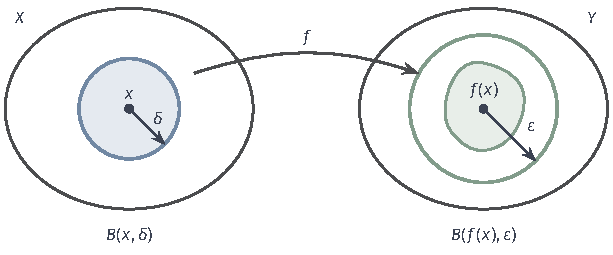
\includegraphics[width=103.738mm]{figures/04-spaces-measures-and-geometry/01-topology-and-metric/tikz/mmap-epsilon-delta/figure.pdf}
  \caption{一点连续的距离判据。蓝色球是输入端的$B(x,\delta)$，绿色圆是输出端的$B(f(x),\varepsilon)$，绿色填充区域是像$f(B(x,\delta))$。给定$\varepsilon$后，要找到足够小的$\delta$，使像完全落在绿色圆内；像本身不必是球。}
  \label{fig:mmap-epsilon-delta}
\end{BookInlineFigure}

把“$f(U)\subseteq V$”中的邻域都换成球，就得到熟悉的$\varepsilon$-$\delta$条件。

\begin{theorem}[一点连续的距离判据]
\label{thm:mmap-epsilon-delta}
$f$在$x\in X$处连续，当且仅当对任意$\varepsilon>0$，存在$\delta>0$，使得对所有$x'\in X$，
\begin{equation}
 d_X(x,x')<\delta
 \quad\Longrightarrow\quad
 d_Y(f(x),f(x'))<\varepsilon.
 \label{eq:mmap-epsilon-delta}
\end{equation}
\end{theorem}

\begin{proof}
设$f$在$x$处连续，给定$\varepsilon>0$。球$B(f(x),\varepsilon)$是$f(x)$的邻域，按一点连续的定义，有$x$的邻域$U$使
\[
 f(U)\subseteq B(f(x),\varepsilon).
\]
度量空间中$x$的邻域包含某个球，设$B(x,\delta)\subseteq U$。这个$\delta$满足式~\eqref{eq:mmap-epsilon-delta}。

反过来，设距离条件成立，$V$是$f(x)$的邻域。$V$包含某个球$B(f(x),\varepsilon)$，对这个$\varepsilon$取条件中的$\delta$，令$U=B(x,\delta)$。则$U$是$x$的邻域，并且
\[
 f(U)\subseteq B(f(x),\varepsilon)\subseteq V.
\]
所以$f$在$x$处连续。
\end{proof}

条件中的$\delta$可以依赖$x$，也可以依赖$\varepsilon$。它回答的问题是：输出允许的误差已经给定，输入需要控制在多小的范围内。前面的$x^2$例子里，$x=1$时用的是$\delta=\min\{1,\varepsilon/3\}$，换到别的点，这个公式就要跟着改变。

下一个定理说明，每一点都满足这句保证，恰好就是第~\ref{chap:topological-spaces}章定义的连续映射。

\begin{theorem}[逐点连续与开集原像]
\label{thm:mmap-pointwise-open-preimage}
$f$在$X$的每一点满足定理~\ref{thm:mmap-epsilon-delta}的距离条件，当且仅当$Y$中每个开集的原像都是$X$中的开集。
\end{theorem}

\begin{proof}
设距离条件处处成立，$U\subseteq Y$是开集，$x\in f^{-1}(U)$。$U$是开集，所以可取$\varepsilon>0$使$B(f(x),\varepsilon)\subseteq U$。再取对应的$\delta$，距离条件给出
\[
 f(B(x,\delta))\subseteq B(f(x),\varepsilon)\subseteq U,
\]
也就是$B(x,\delta)\subseteq f^{-1}(U)$。$x$是$f^{-1}(U)$中任意一点，所以$f^{-1}(U)$是开集。

反过来，设开集的原像都是开集。对$x\in X$和$\varepsilon>0$，集合$f^{-1}(B(f(x),\varepsilon))$是包含$x$的开集，所以其中有某个球$B(x,\delta)$。这个$\delta$满足式~\eqref{eq:mmap-epsilon-delta}。
\end{proof}

由$f^{-1}(Y\setminus F)=X\setminus f^{-1}(F)$，开集原像为开集等价于闭集原像为闭集，后者常用来判断集合是闭集。例如$g(\bm x)=x_1^2+x_2^2$在$(\mathbb R^2,d_2)$上连续，于是单位圆周是闭集，原因是
\[
 S^1=g^{-1}(\{1\}),
\]
单点集$\{1\}$是$\mathbb R$中的闭集；同样，圆盘$\{\bm x:g(\bm x)\leq4\}=g^{-1}((-\infty,4])$也是闭集。

连续性只保证原像保持开闭，不保证像保持开闭。$f(x)=x^2$把开区间$(-1,1)$映成$[0,1)$，后者在$\mathbb R$中不是开集，因为$0$处没有向左的邻域。$f(x)=e^x$把闭集$\mathbb R$映成$(0,\infty)$，后者不是闭集，因为$0$在它的闭包中。把开集映成开集的映射称为开映射，这是另一回事。

距离函数是最常用的连续函数。固定$z\in X$，由三角不等式$d(x,z)\leq d(x,x')+d(x',z)$，交换$x,x'$后合起来得到
\[
 \lvert d(x,z)-d(x',z)\rvert\leq d(x,x').
\]

对非空集合$A\subseteq X$，每个$a\in A$满足$d(x,A)\leq d(x,a)\leq d(x,x')+d(x',a)$。对$a$取下确界，再交换$x,x'$，得到
\[
 \lvert d(x,A)-d(x',A)\rvert\leq d(x,x').
\]

这两个函数都可以取$\delta=\varepsilon$，并且这个$\delta$对所有点通用，这种通用性下一节将命名为均匀连续。它们的零点集分别是$\{z\}$和$\overline A$，这再次说明单点集与闭包都是闭集。

\subsection{连续性的序列判据}
\label{sec:mmap-sequential-continuity}

对每个$\varepsilon$找$\delta$，有时不如直接看点列方便。上一章已经用点列描述了闭包，度量空间中点列同样足以探测连续性。

\begin{theorem}[连续性的序列判据]
\label{thm:mmap-sequential-continuity}
$f$在$x$处连续，当且仅当对$X$中每个满足$x_n\to x$的点列，都有$f(x_n)\to f(x)$。
\end{theorem}

\begin{proof}
设$f$在$x$处连续，$x_n\to x$。给定$\varepsilon>0$，取距离条件中的$\delta$，再取$N$使$n\geq N$时$d(x_n,x)<\delta$。这些$n$都满足
\[
 d(f(x_n),f(x))<\varepsilon,
\]
所以$f(x_n)\to f(x)$。

反方向用反证法。设$f$在$x$处不连续，按定理~\ref{thm:mmap-epsilon-delta}，存在某个$\varepsilon>0$，使任何$\delta>0$都不满足条件。对每个$n$取$\delta=1/n$，这一失败给出一点$x_n$，满足
\[
 d(x_n,x)<\frac1n,\qquad d(f(x_n),f(x))\geq\varepsilon.
\]
于是$x_n\to x$，而$f(x_n)$不趋于$f(x)$，与假设矛盾。
\end{proof}

序列判据特别适合否定连续性：只需找到一个趋于$x$、像却不趋于$f(x)$的点列。在$\mathbb R^2$上令
\[
 f(\bm x)=\frac{x_1x_2}{x_1^2+x_2^2}\quad(\bm x\neq\bm 0),\qquad f(\bm 0)=0.
\]

沿对角线上的点$\bm x_n=(1/n,1/n)$，分子是$1/n^2$，分母是$2/n^2$，于是
\[
 f(\bm x_n)=\frac12,\qquad \bm x_n\to\bm 0,
\]
像不趋于$f(\bm 0)=0$，所以$f$在原点不连续。沿坐标轴趋近时函数值恒为$0$，只看这个方向会得出错误结论：判据要求每一个趋于该点的点列都保持极限。

序列判据也可以用来肯定连续性。设$f:X\to Y$在$x$处连续，$g:Y\to Z$在$f(x)$处连续。若$x_n\to x$，则$f(x_n)\to f(x)$，再由$g$的连续性得
\[
 g(f(x_n))\to g(f(x)).
\]
所以$g\circ f$在$x$处连续。第~\ref{chap:topological-spaces}章已用开集原像证明了复合映射的连续性，这里是它在度量空间中的另一种读法。

在一般拓扑空间中，正方向仍然成立。若$f$连续且$x_n\to x$，对$f(x)$的邻域$V$，$f^{-1}(V)$是$x$的邻域，点列最终落在其中，所以$f(x_n)$最终落在$V$中。

反方向依赖于点列能否探测拓扑。上面的证明取$\delta=1/n$依次选点，用的正是每点有可数个球作邻域基；第~\ref{chap:topological-spaces}章的余可数拓扑没有这样的邻域基，那里给出了保持全部收敛点列、却不连续的映射。

\section{均匀连续与Lipschitz连续}
\label{sec:mmap-uniform-lipschitz}

连续性允许$\delta$随输入点改变。处理单个点附近的问题时这无关紧要，但处理柯西列、稠密集上的延拓或迭代误差时，点列的各项散布在不同位置，需要一个对整个定义域都有效的阈值，最好还能给出输出误差是输入误差的多少倍。本节依次加强条件：均匀连续要求阈值与位置无关，Lipschitz连续要求误差按固定比例放大。最后说明紧定义域上连续自动升级为均匀连续，却不能自动升级为Lipschitz连续。卷一在实轴区间上讨论过这些概念，可参考\BookChapterRef{chap:limits-continuity}{卷一“极限与连续”章}，这里推广到度量空间。

\subsection{均匀连续}
\label{sec:mmap-uniform-continuity}

先看阈值怎样依赖位置。在$\mathbb R$上取$f(x)=x^2$，有$\lvert f(x')-f(x)\rvert=\lvert x'-x\rvert\,\lvert x'+x\rvert$。在$x$附近要使输出误差小于$1$，输入误差大约要小于$1/(2\lvert x\rvert)$，$x$越大，允许的输入误差越小。换到区间$[0,1]$上，$\lvert x'+x\rvert\leq2$，于是$\lvert f(x')-f(x)\rvert\leq2\lvert x'-x\rvert$，取$\delta=\varepsilon/2$对区间中所有点都有效。

\begin{definition}[均匀连续]
\label{def:mmap-uniform-continuity}
若对任意$\varepsilon>0$，存在$\delta>0$，使得对所有满足$d_X(x,x')<\delta$的$x,x'\in X$，都有$d_Y(f(x),f(x'))<\varepsilon$，则称$f$\term{均匀连续}（uniformly continuous）。卷一称之为一致连续。
\end{definition}

与逐点连续相比，变化只在量词的次序：逐点连续是“对每个$x$和$\varepsilon$，存在$\delta$”，均匀连续是“对每个$\varepsilon$，存在$\delta$，对所有$x,x'$”。否定均匀连续时，常用点对序列：若存在$\varepsilon>0$及点列$x_n,x_n'$，使$d(x_n,x_n')\to0$而$d(f(x_n),f(x_n'))\geq\varepsilon$，则$f$不均匀连续，因为任何$\delta$都会被某个$d(x_n,x_n')<\delta$的点对打破。对$\mathbb R$上的$x^2$，取$x_n=n$，$x_n'=n+1/n$，则$\lvert x_n-x_n'\rvert=1/n\to0$，而$\lvert x_n'^2-x_n^2\rvert=2+1/n^2\geq2$。

均匀连续的直接用处是保持柯西列。

\begin{theorem}[均匀连续映射保持柯西列]
\label{thm:mmap-uniform-cauchy-image}
若$f$均匀连续，$(x_n)$是$X$中的柯西列，则$(f(x_n))$是$Y$中的柯西列。
\end{theorem}

\begin{proof}
对$\varepsilon>0$取均匀连续的$\delta$，再取$N$使$m,n\geq N$时$d(x_m,x_n)<\delta$，则这些$m,n$满足$d(f(x_m),f(x_n))<\varepsilon$。
\end{proof}

仅有连续性不够。$f(x)=1/x$在$(0,1)$上连续，$x_n=1/(n+1)$是柯西列，像$n+1$却不是柯西列；按定理，这也说明$1/x$在$(0,1)$上不均匀连续。第~\ref{sec:mmap-extension}节把均匀连续映射从稠密子集延拓出去，依靠的正是这一定理：逼近同一点的柯西列，其像也是柯西列。

\subsection{Lipschitz连续}
\label{sec:mmap-lipschitz}

均匀连续只说存在$\delta$，没有说$\delta$与$\varepsilon$的关系。若输出误差不超过输入误差的固定倍数，误差估计就可以直接写出来。

\begin{definition}[Lipschitz连续]
\label{def:mmap-lipschitz}
若存在有限常数$L\geq0$，使对所有$x,x'\in X$有
\begin{equation}
d_Y(f(x),f(x'))\leq L\,d_X(x,x'),
\label{eq:mmap-lipschitz}
\end{equation}
则称$f$为\term{Lipschitz连续}（Lipschitz continuous）的，$L$称为一个Lipschitz常数。满足式\eqref{eq:mmap-lipschitz}的最小常数记为
\begin{equation*}
\operatorname{Lip}(f)=\sup_{x\neq x'}\frac{d_Y(f(x),f(x'))}{d_X(x,x')},
\end{equation*}
称为$f$的\term{Lipschitz常数}（Lipschitz constant）。
\end{definition}

Lipschitz连续蕴含均匀连续：$L>0$时取$\delta=\varepsilon/L$，$L=0$时$f$为常值。它还给出可以计算的误差放大界：输入误差为$\eta$时，输出误差至多为$L\eta$。若$f:X\to Y$与$g:Y\to Z$都Lipschitz连续，则
\begin{equation*}
d(g(f(x)),g(f(x')))\leq\operatorname{Lip}(g)\,d(f(x),f(x'))\leq\operatorname{Lip}(g)\operatorname{Lip}(f)\,d(x,x'),
\end{equation*}
所以$\operatorname{Lip}(g\circ f)\leq\operatorname{Lip}(g)\operatorname{Lip}(f)$：多步计算的误差放大倍数至多相乘。

常见的Lipschitz映射有几类。距离函数$x\mapsto d(x,A)$的Lipschitz常数不超过$1$。区间上可微且$\lvert f'\rvert\leq L$的实函数满足$\lvert f(x)-f(x')\rvert=\lvert f'(\xi)\rvert\,\lvert x-x'\rvert\leq L\lvert x-x'\rvert$，这里用到中值定理，可参考\BookChapterRef{chap:univariate-differentiation}{卷一“一元函数的微分”章}；前面的$x^2$在$[0,1]$上就有$L=2$。矩阵$\bm A$定义的线性映射满足$\lVert\bm A\bm x-\bm A\bm y\rVert\leq\lVert\bm A\rVert\,\lVert\bm x-\bm y\rVert$，其中$\lVert\bm A\rVert$是诱导的算子范数，可参考\BookChapterRef{chap:normed-inner-product-spaces}{卷二“赋范空间与内积空间”章}。

均匀连续不必Lipschitz连续。在$[0,1]$上取$f(x)=\sqrt x$。对$0\leq y\leq x$，$(\sqrt y+\sqrt{x-y})^2=x+2\sqrt{y(x-y)}\geq x$，所以$\sqrt x-\sqrt y\leq\sqrt{x-y}$，取$\delta=\varepsilon^2$即得均匀连续。但$\sqrt x/x=1/\sqrt x$在$x\to0^+$时无界，没有有限的$L$满足$\sqrt x-\sqrt0\leq Lx$。平方根在$0$附近把输入误差$\eta$放大为$\sqrt\eta$，放大倍数$1/\sqrt\eta$没有上界。

$L<1$的自映射把任意两点的距离按固定比例缩小，这是第~\ref{sec:mmap-contraction}节压缩迭代的出发点。

\subsection{紧空间上的均匀连续性}
\label{sec:mmap-compact-uniform}

前面的反例$x^2$与$1/x$分别定义在无界的$\mathbb R$和不包含端点的$(0,1)$上，都不是紧空间。紧性恰好排除了阈值随位置无限缩小的情形。

\begin{theorem}[紧空间上的均匀连续性]
\label{thm:mmap-compact-uniform}
若$X$是紧致度量空间，$f:X\to Y$连续，则$f$均匀连续。
\end{theorem}

\begin{proof}
若不然，存在$\varepsilon>0$及点列$x_n,x_n'$，使$d(x_n,x_n')<1/n$而$d(f(x_n),f(x_n'))\geq\varepsilon$。按第~\ref{chap:metric-spaces}章，紧致度量空间序列紧致，取子列$x_{n_k}\to x\in X$，则$d(x'_{n_k},x)\leq d(x'_{n_k},x_{n_k})+d(x_{n_k},x)\to0$。由$f$在$x$处连续及序列判据，$f(x_{n_k})$与$f(x'_{n_k})$都趋于$f(x)$，于是$d(f(x_{n_k}),f(x'_{n_k}))\to0$，与$\geq\varepsilon$矛盾。
\end{proof}

也可以用开覆盖证明：对每个$x$取使$f(B(x,\delta_x))\subseteq B(f(x),\varepsilon/2)$的$\delta_x$，球族$\{B(x,\delta_x)\}$的Lebesgue数就是对全空间通用的阈值。两种证明都把逐点的阈值变成有限个或一个收敛子列能控制的情形。

紧性是充分条件，不是必要条件：恒等映射在$\mathbb R$上均匀连续，而$\mathbb R$不紧。定理也只给出统一的阈值，不给出Lipschitz常数。$[0,1]$紧致，$\sqrt x$在其上连续因而均匀连续，但上一小节已说明它不Lipschitz连续。均匀连续保证存在随$\varepsilon$变化的$\delta(\varepsilon)$，Lipschitz连续则要求$\delta$可以取成$\varepsilon$的固定倍数。

\section{映射列的收敛}
\label{sec:mmap-map-sequences}

用多项式、截断级数或迭代格式逼近一个映射时，得到的是一列映射$f_1,f_2,\ldots$。说它们“趋于”$f$，可以只要求每个固定输入处的输出趋于$f$的值，也可以要求同一个序号对全部输入都达到给定精度。两种要求的差别决定了极限能否继承连续性。本节设$X$是集合（讨论连续性时是拓扑空间），$(Y,d)$是度量空间，$f_n,f:X\to Y$。先定义两种收敛并说明一致距离的适用范围，再证明一致极限保持连续，最后说明目标空间完备时，一致柯西列必有一致极限。

\subsection{逐点收敛与一致收敛}
\label{sec:mmap-pointwise-uniform}

两种收敛的区别在于“达到精度所需的序号”是否允许随输入改变。

\begin{definition}[逐点收敛与一致收敛]
\label{def:mmap-pointwise-uniform}
若对每个$x\in X$，当$n\to\infty$时都有$d(f_n(x),f(x))\to0$，即对每个$x$和$\varepsilon>0$存在$N$（可依赖于$x$）使$n\geq N$时$d(f_n(x),f(x))<\varepsilon$，则称$(f_n)$\term{逐点收敛}（pointwise convergence）于$f$。若对每个$\varepsilon>0$存在不依赖于$x$的$N$，使$n\geq N$时对所有$x\in X$都有$d(f_n(x),f(x))<\varepsilon$，则称$(f_n)$\term{一致收敛}（uniform convergence）于$f$。
\end{definition}

在$[0,1]$上取$f_n(x)=x^n$。对$x\in[0,1)$有$x^n\to0$，而$f_n(1)=1$，所以逐点极限是$f(x)=0$（$x<1$）、$f(1)=1$。所需序号随$x$变化：要使$x^n<0.01$，$x=0.9$时需要$n\geq44$，因为$\ln0.01/\ln0.9\approx43.7$；$x=0.99$时需要$n\geq459$，因为$\ln0.01/\ln0.99\approx458.2$。越接近$1$，所需序号越大，没有一个$N$对全部$x\in[0,1)$有效：对任何$n$，$\sup_{0\leq x<1}x^n=1$。所以这个映射列不一致收敛。限制到$[0,1/2]$上，$\sup_{0\leq x\leq1/2}x^n=2^{-n}\to0$，就一致收敛于$0$。

一致收敛可以用一个量来概括。令
\begin{equation}
d_\infty(f,g)=\sup_{x\in X}d(f(x),g(x))\in[0,\infty],
\label{eq:mmap-uniform-distance}
\end{equation}
则$f_n$一致收敛于$f$当且仅当$d_\infty(f_n,f)\to0$。但$d_\infty$可能取值$\infty$：在$\mathbb R$上，$f(x)=x$与$g(x)=0$的上确界距离是$\infty$。因此它不能在全体映射上当作通常的度量。

把映射限制在像集有界的映射上，问题就消失了。若$f(X)$含于$Y$的某个球，称$f$为\term{有界映射}（bounded map），记全体有界映射为$B(X,Y)$。对$f,g\in B(X,Y)$，$f(X)\subseteq B(y_1,r_1)$、$g(X)\subseteq B(y_2,r_2)$，则$d(f(x),g(x))<r_1+d(y_1,y_2)+r_2$，所以$d_\infty(f,g)<\infty$。三角不等式逐点成立再取上确界，$d_\infty(f,h)\leq d_\infty(f,g)+d_\infty(g,h)$，零距离判定也逐点成立，所以$d_\infty$是$B(X,Y)$上的度量，称为\term{一致度量}（uniform metric）。在一般映射上谈一致收敛时，仍然使用定义~\ref{def:mmap-pointwise-uniform}的$\varepsilon$-$N$表述，只要求$d_\infty(f_n,f)$最终有限并趋于零。

\subsection{一致极限的连续性}
\label{sec:mmap-uniform-limit-continuity}

$x^n$的例子中，每个$f_n$都连续，逐点极限却在$x=1$处跳跃。一致收敛排除了这种情形，证明只需把误差分成三段。

\begin{theorem}[一致极限保持连续]
\label{thm:mmap-uniform-limit-continuous}
设$X$是拓扑空间，$(Y,d)$是度量空间，$f_n:X\to Y$连续，并且一致收敛于$f$。则$f$连续。
\end{theorem}

\begin{proof}
设$V\subseteq Y$是开集，$x\in f^{-1}(V)$。取$\varepsilon>0$使$B(f(x),\varepsilon)\subseteq V$，再取$N$使对所有$x'\in X$都有$d(f_N(x'),f(x'))<\varepsilon/3$。$f_N$连续，所以$U=f_N^{-1}\bigl(B(f_N(x),\varepsilon/3)\bigr)$是含$x$的开集。对$x'\in U$，
\begin{equation*}
\begin{aligned}
d(f(x'),f(x))
&\leq d(f(x'),f_N(x'))+d(f_N(x'),f_N(x))+d(f_N(x),f(x))\\
&<\tfrac\varepsilon3+\tfrac\varepsilon3+\tfrac\varepsilon3=\varepsilon,
\end{aligned}
\end{equation*}
所以$U\subseteq f^{-1}(V)$。$f^{-1}(V)$的每个点都有含于其中的开集，它是开集。
\end{proof}

三段误差中，首尾两段由一致收敛控制，并且用的是同一个$N$；中间一段由单个$f_N$的连续性控制。若只有逐点收敛，首段$d(f(x'),f_N(x'))$所需的$N$随$x'$变化，无法与中间一段的邻域$U$同时取定，$x^n$正是这样失败的。

定理的条件很少：定义域只需是拓扑空间，不要求紧致；目标空间只需是度量空间，不要求完备，因为极限$f$已经假定存在。一致收敛也只是充分条件：$x^n$在$[0,1)$上逐点收敛于连续函数$0$，但不一致收敛。

\subsection{一致柯西列的极限}
\label{sec:mmap-uniform-cauchy}

上一小节假定了极限$f$存在。和点列一样，实际中往往只能看到映射列的后项彼此接近，需要从这一点推出极限存在。

\begin{definition}[一致柯西列]
\label{def:mmap-uniform-cauchy}
若对任意$\varepsilon>0$，存在$N$，使$m,n\geq N$时对所有$x\in X$都有$d(f_m(x),f_n(x))<\varepsilon$，则称$(f_n)$为\term{一致柯西列}（uniformly Cauchy sequence）。
\end{definition}

\begin{theorem}[一致柯西列的一致极限]
\label{thm:mmap-uniform-cauchy-limit}
设$(Y,d)$完备，$(f_n)$是$X\to Y$的一致柯西列。则存在$f:X\to Y$，使$f_n$一致收敛于$f$。
\end{theorem}

\begin{proof}
对每个固定的$x$，$(f_n(x))$是$Y$中的柯西列，由完备性收敛，记极限为$f(x)$。给定$\varepsilon>0$，取$N$使$m,n\geq N$时对所有$x$有$d(f_n(x),f_m(x))<\varepsilon$。固定$n\geq N$和$x$，令$m\to\infty$。由第~\ref{chap:metric-spaces}章的不等式$\lvert d(a,b)-d(a,c)\rvert\leq d(b,c)$，$d(f_n(x),f_m(x))\to d(f_n(x),f(x))$，所以$d(f_n(x),f(x))\leq\varepsilon$。这对所有$x$和所有$n\geq N$成立，即一致收敛。
\end{proof}

证明的顺序值得注意：先逐点取极限得到候选的$f$，再在不等式中让后项趋于极限，把对所有$x$统一的估计传给$f$。目标空间的完备性不可省略。取$Y=\mathbb Q$，$f_n$为常值映射，取值为$\sqrt2$的第$n$个十进制截断，它们是一致柯西列，却没有取值在$\mathbb Q$中的极限。

把本小节与上一小节合起来，就得到函数空间完备性的共同依据。

\begin{theorem}[有界映射空间的完备性]
\label{thm:mmap-bounded-maps-complete}
设$(Y,d)$完备。则$(B(X,Y),d_\infty)$完备。若$X$是拓扑空间，有界连续映射全体$C_b(X,Y)$是$B(X,Y)$的闭子集，因而也完备。
\end{theorem}

\begin{proof}
$B(X,Y)$中关于$d_\infty$的柯西列就是一致柯西列，由定理~\ref{thm:mmap-uniform-cauchy-limit}一致收敛于某个$f$。取$N$使$d_\infty(f_N,f)\leq1$，$f_N$的像含于某个球$B(y,r)$，则$f$的像含于$B(y,r+1)$，$f\in B(X,Y)$，并且$d_\infty(f_n,f)\to0$。若各$f_n$还连续，由定理~\ref{thm:mmap-uniform-limit-continuous}，$f$连续。这说明$C_b(X,Y)$包含其中点列的极限，是闭集；按第~\ref{chap:metric-spaces}章，完备空间的闭子空间完备。
\end{proof}

$X$紧致时，连续映射的像是紧集，因而有界，所以$C_b(X,Y)$就是全体连续映射$C(X,Y)$。例如$C([0,1],\mathbb R)$在一致度量下完备。检验具体的函数列时，常常先估计一致柯西性。在$[0,1]$上令$s_n(x)=\sum_{k=1}^nx^k/k^2$。对$m>n$，
\begin{equation*}
\lvert s_m(x)-s_n(x)\rvert\leq\sum_{k=n+1}^m\frac1{k^2}\leq\sum_{k=n+1}^m\Bigl(\frac1{k-1}-\frac1k\Bigr)<\frac1n,
\end{equation*}
上界与$x$无关，所以$(s_n)$是一致柯西列，一致收敛于一个连续函数。第~\ref{chap:normed-spaces}章核验具体函数空间的完备性时，反复使用的就是这一模式：先逐点取极限，再证明极限属于所考察的空间。

\section{等度连续性}
\label{sec:mmap-equicontinuity}

上一节研究的是一列映射趋于一个极限；有时我们关心的是一整族映射作为整体有多“规整”。例如一族函数各自连续，但随着下标增大越来越陡，它们在同一个输入点附近需要的阈值就越来越小。

均匀连续说的是$\delta$与位置无关，等度连续把这个想法换成$\delta$与族中的成员无关。本节给出定义，并证明在紧定义域上，两种“无关”可以同时实现。

\paragraph{等度连续的定义}
在$[0,1]$上看映射族$\mathcal F=\{x^n:n\geq1\}$，每个$x^n$都连续。先看$x_0=1$，取$\varepsilon=1/2$。对任何$\delta\in(0,1)$，令$x=1-\delta/2$，则$\lvert x-1\rvert<\delta$，而$(1-\delta/2)^n\to0$，所以$n$充分大时
\[
 \lvert x^n-1^n\rvert>\frac12.
\]
没有一个$\delta$对全族有效。

在$x_0=1/2$处情况不同，这里可以把全族分成两组来处理。取$\varepsilon=1/10$，先限制$\lvert x-1/2\rvert<1/4$，此时$x<3/4$，于是
\[
 \lvert x^n-(1/2)^n\rvert\leq(3/4)^n.
\]
由$(3/4)^9\approx0.075$，$n\geq9$的成员在这个半径上已经满足要求。

剩下$n=1,\ldots,8$这八个成员，用中值定理估计。对$x,x'\in[0,3/4]$，
\[
 \lvert x^n-x'^n\rvert\leq n(3/4)^{n-1}\lvert x-x'\rvert\leq\frac{27}{16}\lvert x-x'\rvert,
\]
这里系数$n(3/4)^{n-1}$在$n=3,4$处取最大值$27/16=1.6875$。

要使右端小于$1/10$，只需$\lvert x-x'\rvert<8/135$，于是全族共用的半径可以取
\[
 \delta=\frac1{17}.
\]
验算：$1/17<8/135$，并且$1/17<1/4$，所以这个$\delta$对全部$n$都有效。

\begin{definition}[等度连续]
\label{def:mmap-equicontinuous}
设$\mathcal F$是一族映射$X\to Y$，$x\in X$。若对任意$\varepsilon>0$，存在$\delta>0$，使得对所有$f\in\mathcal F$和所有$x'\in X$，
\begin{equation}
 d(x,x')<\delta
 \quad\Longrightarrow\quad
 d(f(x),f(x'))<\varepsilon,
 \label{eq:mmap-equicontinuous}
\end{equation}
则称$\mathcal F$在$x$处\term{等度连续}（equicontinuous）。若$\mathcal F$在$X$的每一点等度连续，称$\mathcal F$在$X$上等度连续。若$\delta$还可以对所有$x$通用，称$\mathcal F$\term{一致等度连续}（uniformly equicontinuous）。
\end{definition}

上面的$\{x^n\}$在每个$x_0\in[0,1)$处等度连续：取$\delta_0=(1-x_0)/2$，$B(x_0,\delta_0)$内的点都不超过$r=(1+x_0)/2<1$，$r^n$最终小于$\varepsilon$，前面有限个成员再各取一个半径，与$\delta_0$取最小值即可。在$x_0=1$处不等度连续。

每个成员连续，只说明每个$f$都有自己的$\delta_f$；等度连续要求这些$\delta_f$有正的下界。有限族总是满足这一点，取有限个$\delta_f$的最小值就行；无限族则可能不满足，下面的例子把两种情形并排放在一起。

\paragraph{等度连续的例子}
共同的Lipschitz常数给出最简单的等度连续族。若每个$f\in\mathcal F$都满足$d(f(x),f(x'))\leq Ld(x,x')$，取$\delta=\varepsilon/L$，它对所有成员和所有点都有效，所以族一致等度连续。例如平移族$\{x\mapsto\sin(x+c):c\in\mathbb R\}$，每个成员的导数绝对值不超过$1$，是$1$-Lipschitz族。

频率不断增大的族则不然。$\{x\mapsto\sin(nx):n\geq1\}$在$0$处不等度连续：对任何$\delta>0$，取$n>\pi/(2\delta)$，点$x'=\pi/(2n)$满足$\lvert x'\rvert<\delta$，而
\[
 \lvert\sin(nx')-\sin0\rvert=1.
\]

图~\ref{fig:mmap-equicontinuity}并排画出这两族。左边的曲线在宽度$\delta$的窗口内一起缓慢变化，右边的曲线随$n$增大越来越早地冲到$1$，无论窗口多窄，总有成员在窗口内完成一次满振幅。

\begin{BookInlineFigure}
  \centering
  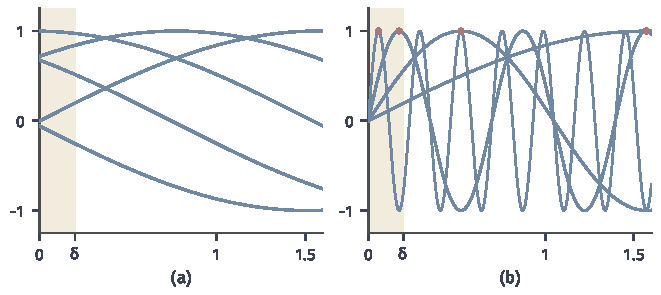
\includegraphics[width=112mm]{figures/04-spaces-measures-and-geometry/01-topology-and-metric/matplotlib/mmap-equicontinuity/figure.pdf}
  \caption{等度连续与不等度连续。(a) 平移族$\sin(x+c)$，$c=0,0.8,1.6,2.4,3.2$，导数绝对值不超过$1$，在宽度$\delta=0.2$的窗口（黄色）内每条曲线的变化不超过$0.2$。(b) $\sin(nx)$，$n=1,3,9,27$，红点是首次到达$1$的位置$x=\pi/(2n)$，当$n$足够大时落进任何给定的窗口。}
  \label{fig:mmap-equicontinuity}
\end{BookInlineFigure}

\paragraph{紧定义域上的统一半径}
均匀连续与连续之间的关系，对映射族同样成立：在紧定义域上，逐点的等度连续可以升级为一致的等度连续。

\begin{theorem}[紧空间上的一致等度连续]
\label{thm:mmap-compact-uniform-equicontinuous}
设$X$是紧致度量空间，$\mathcal F$是在$X$上等度连续的映射族。则$\mathcal F$一致等度连续。
\end{theorem}

\begin{proof}
反证。若结论不成立，存在$\varepsilon>0$，以及$f_n\in\mathcal F$和点列$x_n,x_n'$，使
\[
 d(x_n,x_n')<\frac1n,\qquad d(f_n(x_n),f_n(x_n'))\geq\varepsilon.
\]

由序列紧致性，取子列$x_{n_k}\to x\in X$，由三角不等式，$x'_{n_k}$也趋于$x$。在$x$处用等度连续，取对应于$\varepsilon/2$的$\delta$。

当$k$充分大时，$x_{n_k}$与$x'_{n_k}$都落在$B(x,\delta)$中，于是由三角不等式，
\[
 \begin{aligned}
 d(f_{n_k}(x_{n_k}),f_{n_k}(x'_{n_k}))
 &\leq d(f_{n_k}(x_{n_k}),f_{n_k}(x))\\
 &\quad+d(f_{n_k}(x),f_{n_k}(x'_{n_k}))<\varepsilon.
 \end{aligned}
\]
这与不小于$\varepsilon$矛盾。
\end{proof}

证明与定理~\ref{thm:mmap-compact-uniform}几乎相同，区别只在于映射$f_{n_k}$也随下标变化；等度连续保证在极限点$x$附近，所有成员共用同一个$\delta$。紧性在这里同样不可省略：$\{x^n\}$在$[0,1)$上等度连续，但不一致等度连续，因为越接近$1$，所需的$\delta$越小。

等度连续性的主要用途是判断函数族在一致度量下是否相对紧。等度连续控制函数在定义域上的“摆动”，有界性控制函数值的范围，二者合起来可以用有限张代表表在给定精度内覆盖整个族。这一判据及其覆盖数估计在第~\ref{chap:function-class-covers}章给出。

\section{度量空间的比较}
\label{sec:mmap-comparison}

两个度量空间“一样”是什么意思，取决于我们要保留什么。若要保留每一对点的距离，就要求映射保持距离；若只要保留开集、收敛与紧性，同胚就够了；若要保留柯西列与完备性，或者进一步保留误差的数量级，就需要介于两者之间的条件。

本节先研究保持距离的映射，再说明同胚为什么不保留完备性，最后在同一集合的两个度量之间，把“等价”分成三个强弱不同的层次。

\subsection{等距映射}
\label{sec:mmap-isometry}

最强的比较是要求距离完全不变。

\begin{definition}[等距映射]
\label{def:mmap-isometry}
若映射$f:X\to Y$对所有$x,x'\in X$满足
\begin{equation}
 d_Y(f(x),f(x'))=d_X(x,x'),
 \label{eq:mmap-isometry}
\end{equation}
则称$f$为\term{等距映射}（isometric mapping），也称\term{等距嵌入}（isometric embedding）。若等距映射还是满射，称$X$与$Y$等距。
\end{definition}

等距映射自动是单射：$f(x)=f(x')$时，由式~\eqref{eq:mmap-isometry}得$d(x,x')=0$。它是$1$-Lipschitz的，因而连续。由于距离不变，$(x_n)$是柯西列当且仅当$(f(x_n))$是柯西列，$x_n\to x$当且仅当$f(x_n)\to f(x)$。

把$f$看成$X$到像集$f(X)$的双射，它的逆也是等距映射。于是$X$完备当且仅当子空间$f(X)$完备，$X$紧致当且仅当$f(X)$紧致：这些性质都只用距离和点列描述，经等距映射原样搬运。

满射与否区分了“相同”与“嵌入”。平面的旋转和平移都是$(\mathbb R^2,d_2)$到自身的满射等距映射，旋转前后的图形作为度量空间无法区分。$t\mapsto(t,0)$是$\mathbb R$到$\mathbb R^2$的等距映射，但不是满射，它把实轴嵌成平面中的一条直线。第~\ref{chap:metric-spaces}章完备化中的$\iota:X\to\hat X$也是等距嵌入，它的像稠密，只有$X$本身完备时才是满射。

无限空间可以等距地嵌入自身的真子集，有限集做不到这一点。在自然数集$\{1,2,\ldots\}$上取通常距离，$n\mapsto n+1$保持距离，但像集不含$1$。所以“$X$等距嵌入$Y$且$Y$等距嵌入$X$”不能直接推出两者等距，需要单独核验满射。

\subsection{同胚与度量性质}
\label{sec:mmap-homeomorphism-metric}

第~\ref{chap:topological-spaces}章的同胚是双向连续的双射，它保持一切用开集表述的性质，例如紧致、连通、可分，以及点列的收敛。那里还说明了实轴与开区间同胚，这里取从实轴到开区间的方向：
\begin{equation}
 h:\mathbb R\to(-1,1),\qquad
 h(x)=\frac x{1+\lvert x\rvert},\qquad
 h^{-1}(y)=\frac y{1-\lvert y\rvert}.
 \label{eq:mmap-homeo-h}
\end{equation}

图~\ref{fig:mmap-homeo-line}画出$h$对整数点的作用。两个空间都配上通常的距离$\lvert\cdot\rvert$。上方整数点相邻间距恒为$1$，下方的像却越来越挤，集中到端点$1$。

\begin{BookInlineFigure}
  \centering
  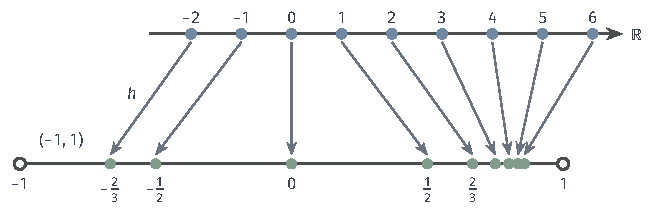
\includegraphics[width=110.659mm]{figures/04-spaces-measures-and-geometry/01-topology-and-metric/tikz/mmap-homeo-line/figure.pdf}
  \caption{同胚$h(x)=x/(1+\lvert x\rvert)$把$\mathbb R$上的整数点（上方，蓝）映到开区间$(-1,1)$内（下方，绿）。上方点列相邻距离恒为$1$，不是柯西列；像点$1-1/n$是柯西列，但极限$1$不在开区间内。}
  \label{fig:mmap-homeo-line}
\end{BookInlineFigure}

$\mathbb R$完备，$(-1,1)$不完备：$y_n=1-1/n$是$(-1,1)$中的柯西列，极限$1$不在其中。用$h^{-1}$搬回实轴，
\[
 h^{-1}(y_n)=\frac{1-1/n}{1/n}=n-1,
\]
相邻两项相距$1$，不是柯西列。同胚把一个柯西列变成了非柯西列，所以柯西性不是拓扑性质，完备性也不是。同样，$(-1,1)$有界、全有界，$\mathbb R$两者都不是，所以有界性与全有界性也不被同胚保持。

换一个角度，同一个集合也可以配上拓扑相同、完备性不同的度量。在$\mathbb R$上令
\[
 d_h(x,y)=\lvert h(x)-h(y)\rvert.
\]
$h$是单射，所以$d_h$是度量；$h:(\mathbb R,d_h)\to(-1,1)$是满射等距映射，所以$(\mathbb R,d_h)$不完备，其中$x_n=n-1$是柯西列而无极限。

另一方面，$h$是通常拓扑下的同胚，$d_h$的开集恰是通常的开集。这就是第~\ref{chap:metric-spaces}章预告的、与通常度量拓扑相同却不完备的度量。

在紧致度量空间之间，这种差别不会出现：紧致蕴含完备且全有界，而紧致是拓扑性质，所以与紧致度量空间同胚的度量空间也完备、全有界。差别只出现在非紧空间中，那里完备性依赖于“无穷远处”的距离怎样度量。

\subsection{同一集合上的度量等价}
\label{sec:mmap-metric-equivalence}

设$d$与$d'$是同一集合$X$上的两个度量。比较它们相当于研究恒等映射$\operatorname{id}:(X,d)\to(X,d')$及其逆满足什么条件。按要求由弱到强，有三种“等价”。

\begin{definition}[度量的三种等价]
\label{def:mmap-metric-equivalence}
设$d,d'$是$X$上的度量。
\begin{enumerate}
\item 若$d$与$d'$诱导相同的开集，即$\operatorname{id}$双向连续，称它们\term{拓扑等价}（topologically equivalent）；
\item 若$\operatorname{id}:(X,d)\to(X,d')$与其逆都均匀连续，称它们\term{一致等价}（uniformly equivalent）；
\item 若存在常数$0<c\leq C$，使对所有$x,y$有
\begin{equation}
 c\,d(x,y)\leq d'(x,y)\leq C\,d(x,y),
 \label{eq:mmap-strong-equivalence}
\end{equation}
即$\operatorname{id}$双向Lipschitz连续，称它们\term{强等价}（strongly equivalent）。
\end{enumerate}
\end{definition}

由Lipschitz连续蕴含均匀连续、均匀连续蕴含连续，强等价蕴含一致等价，一致等价蕴含拓扑等价。三个层次分别保留不同的信息，表~\ref{tab:mmap-metric-equivalence}是一份汇总，下面逐一解释。

\begin{BookInlineTable}
  \centering
  \caption{同一集合上三种度量等价保留的信息}
  \label{tab:mmap-metric-equivalence}
  \begin{tabular}{lll}
    \toprule
    等价层次 & 保留的性质 & 不保留的性质 \\
    \midrule
    拓扑等价 & 收敛点列、紧致、可分 & 柯西列、完备 \\
    一致等价 & 另加柯西列、完备、全有界 & 有界性 \\
    强等价 & 另加有界集、误差尺度 & 常数$c,C$的具体值 \\
    \bottomrule
  \end{tabular}
\end{BookInlineTable}

拓扑等价保留一切拓扑性质。按序列判据，它等价于两个度量下收敛的点列及其极限完全相同，所以紧致、可分以及映射的连续性都不因换用另一个度量而改变。它不保留柯西列：上一小节的$\lvert\cdot\rvert$与$d_h$拓扑等价，但前者完备、后者不完备。

一致等价还保留柯西列与完备性。均匀连续映射把柯西列送到柯西列，恒等映射双向均匀连续，两个度量下的柯西列就相同，而收敛点列本来就相同，所以一个完备当且仅当另一个完备。

它还保留全有界性。给定$\varepsilon$，由$\operatorname{id}:(X,d)\to(X,d')$的均匀连续性取$\delta$，则
\[
 B_d(x,\delta)\subseteq B_{d'}(x,\varepsilon),
\]
$d$下半径$\delta$的有限覆盖就是$d'$下半径$\varepsilon$的覆盖；反方向同理。

一致等价却不保留有界性。$\mathbb R$上的$\lvert x-y\rvert$与$\min\{\lvert x-y\rvert,1\}$在小于$1$的尺度上完全一致，对$\varepsilon<1$取$\delta=\varepsilon$，就得到双向均匀连续。但后者下整个$\mathbb R$有界，而前者下$\mathbb R$无界，所以不存在$c>0$使$\min\{\lvert x-y\rvert,1\}\geq c\lvert x-y\rvert$对所有$x,y$成立。

强等价进一步比较误差的尺度。由式~\eqref{eq:mmap-strong-equivalence}，
\begin{equation}
 B_d(x,r/C)\subseteq B_{d'}(x,r)\subseteq B_d(x,r/c),
 \label{eq:mmap-ball-sandwich}
\end{equation}
所以两个度量下的有界集相同，覆盖数也只差一个尺度因子：
\[
 N^{d'}(C\varepsilon,A)\leq N^{d}(\varepsilon,A),
\]
其中上标表示所用的度量。

$\mathbb R^n$上的$\rho_\infty$与$d_2$是最常见的例子，它们满足
\[
 \rho_\infty(\bm x,\bm y)\leq d_2(\bm x,\bm y)\leq\sqrt n\,\rho_\infty(\bm x,\bm y).
\]

取$n=2$，$d=d_2$，$d'=\rho_\infty$，则$c=1/\sqrt2$，$C=1$。把$r=1$代入式~\eqref{eq:mmap-ball-sandwich}，得
\[
 B_{d_2}(\bm x,1)\subseteq B_{\rho_\infty}(\bm x,1)\subseteq B_{d_2}(\bm x,\sqrt2).
\]
图~\ref{fig:mmap-balls}画出的就是这三个集合：圆盘、外切正方形，以及外接圆盘。

\begin{BookInlineFigure}
  \centering
  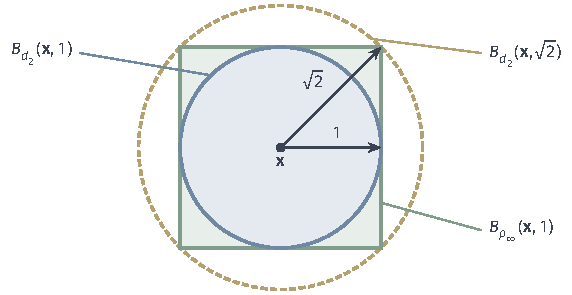
\includegraphics[width=96.852mm]{figures/04-spaces-measures-and-geometry/01-topology-and-metric/tikz/mmap-balls/figure.pdf}
  \caption{$\mathbb R^2$上强等价的两个度量。蓝色圆盘是$d_2$的单位球，绿色正方形是$\rho_\infty$的单位球，黄色虚线圆是$d_2$的半径$\sqrt2$的球。正方形夹在两个圆盘之间，比例由常数$c=1/\sqrt2$，$C=1$决定。}
  \label{fig:mmap-balls}
\end{BookInlineFigure}

卷二证明了有限维空间上任意两个范数诱导的度量都强等价，所以在有限维空间中说“收敛”“有界”“完备”无需指明范数；估计误差时则要记得常数$c,C$可能依赖于维数。这一点在无限维时不再成立，第~\ref{chap:function-normed-spaces}章将看到同一函数空间上不等价的范数。

文献中“等价度量”有时指拓扑等价，有时指强等价。本书遇到这一说法时会写明是哪一种，或直接写出所要求的映射条件。

\section{稠密子集上的映射延拓}
\label{sec:mmap-extension}

只在稠密子集上知道一个映射的值，是常见的情形：先在有理数上定义一个运算，再希望把它推广到全体实数；或者只在有限精度的网格上做过测量，希望确定一个连续量。设$D\subseteq X$稠密，$f:D\to Y$已知。对$x\in X\setminus D$，自然的办法是取$D$中趋于$x$的点列$d_n$，把$f(d_n)$的极限定义为新值。这要求两件事：像点列确实有极限，并且换一个逼近列不会得到不同的结果。本节说明，目标空间完备保证前者，均匀连续保证后者，并且延拓后保留原来的误差控制。

\subsection{延拓的构造}
\label{sec:mmap-extension-construction}

我们先给出定理，再逐步说明每个条件在构造中的作用。

\begin{theorem}[均匀连续映射的延拓]
\label{thm:mmap-extension}
设$D$是度量空间$X$的稠密子集，$Y$是完备度量空间，$f:D\to Y$均匀连续。则存在唯一的连续映射$F:X\to Y$，使$F|_D=f$。
\end{theorem}

\begin{proof}
定义。对$x\in X$，由稠密性和第~\ref{chap:metric-spaces}章的闭包序列判据，取$d_n\in D$使$d_n\to x$。收敛点列是柯西列，均匀连续映射把柯西列送到柯西列，所以$(f(d_n))$是$Y$中的柯西列，由$Y$完备收敛。令$F(x)=\lim_nf(d_n)$。

与逼近列无关。设另有$d_n'\in D$趋于$x$。把两列交替排成新点列$d_1,d_1',d_2,d_2',\ldots$，它仍趋于$x$，于是它的像也是柯西列并收敛到某个$z$。$(f(d_n))$与$(f(d_n'))$都是这个像点列的子列，因而都趋于$z$。所以$F(x)$不依赖于逼近列的选择。

延拓。若$x\in D$，可以取常值逼近列$d_n=x$，得$F(x)=f(x)$。

唯一性。设$G:X\to Y$连续且$G|_D=f$。对$x\in X$及趋于$x$的$d_n\in D$，由序列判据$G(x)=\lim G(d_n)=\lim f(d_n)=F(x)$。$F$本身的连续性在下一小节与误差控制一起证明。
\end{proof}

唯一性的论证只用到$D$稠密与$G$连续，不需要$Y$完备或$f$均匀连续：两个连续映射若在稠密子集上相同，就处处相同。存在性则两个条件都要用，缺一个都会失败。

缺少目标空间的完备性时，像点列可能没有极限。取$X=\mathbb R$、$D=\mathbb Q$、$Y=\mathbb Q$，$f$为$\mathbb Q$上的恒等映射，它是等距映射，当然均匀连续。若有连续延拓$F:\mathbb R\to\mathbb Q$，沿$\sqrt2$的有理截断$q_n$应有$F(\sqrt2)=\lim q_n=\sqrt2$，而$\sqrt2\notin\mathbb Q$。完备性要求作用在目标空间上，定义域$X$完备与否无关紧要。

缺少均匀连续时，不同的逼近列可能给出不同的极限。在$D=\mathbb Q\cap[0,1]$上令$f(q)=0$（$q<1/\sqrt2$）、$f(q)=1$（$q>1/\sqrt2$）。$1/\sqrt2$不是有理数，所以$f$在$D$的每一点附近都是常值，因而连续；但从左、右两侧逼近$1/\sqrt2$的有理数列，像分别恒为$0$与$1$，没有连续延拓到$[0,1]$。这正说明了$f$不均匀连续：两侧的点可以任意接近，函数值却始终相差$1$。

\subsection{延拓后的误差控制}
\label{sec:mmap-extension-error}

延拓不仅存在，还继承原映射在$D$上的误差控制，阈值与常数都不变坏。

\begin{theorem}[延拓保持均匀连续与Lipschitz常数]
\label{thm:mmap-extension-control}
在定理~\ref{thm:mmap-extension}的条件下，设$\varepsilon,\delta>0$满足：$d_1,d_2\in D$且$d(d_1,d_2)<\delta$时$d(f(d_1),f(d_2))<\varepsilon$。则$x,x'\in X$且$d(x,x')<\delta$时$d(F(x),F(x'))\leq\varepsilon$。特别地，$F$均匀连续；若$f$以$L$为Lipschitz常数，则$F$也以$L$为Lipschitz常数。
\end{theorem}

\begin{proof}
取$d_n\to x$，$d_n'\to x'$，$d_n,d_n'\in D$。由三角不等式，$d(d_n,d_n')\to d(x,x')<\delta$，所以$n$充分大时$d(d_n,d_n')<\delta$，从而$d(f(d_n),f(d_n'))<\varepsilon$。令$n\to\infty$，由距离的连续性得$d(F(x),F(x'))\leq\varepsilon$。对任意$\varepsilon$，用$\varepsilon/2$对应的$\delta$，就得到$F$的均匀连续性，特别地$F$连续。

若对$D$中所有点都有$d(f(d_1),f(d_2))\leq L\,d(d_1,d_2)$，则对每个$n$有$d(f(d_n),f(d_n'))\leq L\,d(d_n,d_n')$，两边取极限得$d(F(x),F(x'))\leq L\,d(x,x')$。
\end{proof}

由这两个定理，哪些函数可以由稠密观测唯一确定，答案很清楚。在有理数上给定的函数若在每个有界区间上均匀连续，就唯一地确定了实轴上的连续函数：在每个$[-M,M]$上分别延拓，由唯一性，不同区间上的延拓在公共部分一致；例如多项式$p(q)$在$\mathbb Q\cap[-M,M]$上Lipschitz连续，延拓结果就是同一个多项式在实轴上的取值。反过来，若只知道目标函数连续，在有理点上的值就足以确定它；若函数可以不连续，有理点上的值什么也确定不了，例如在有理点取$0$、在无理点任意取值的函数。

延拓定理还完成了第~\ref{chap:metric-spaces}章留下的一步：完备化在等距意义下唯一。

\begin{theorem}[完备化的唯一性]
\label{thm:mmap-completion-unique}
设$\iota:X\to\hat X$与$j:X\to\tilde X$都是保持距离的映射，$\hat X,\tilde X$完备，像$\iota(X)$与$j(X)$分别稠密。则存在满射等距映射$\Phi:\hat X\to\tilde X$，使$\Phi\circ\iota=j$。
\end{theorem}

\begin{proof}
在稠密子集$\iota(X)$上定义$\phi(\iota(x))=j(x)$，它保持距离，因而是Lipschitz常数为$1$的均匀连续映射。$\tilde X$完备，由定理~\ref{thm:mmap-extension}，$\phi$延拓为连续映射$\Phi:\hat X\to\tilde X$。对$\xi,\eta\in\hat X$，取$\iota(x_n)\to\xi$，$\iota(y_n)\to\eta$，则
\begin{equation*}
\begin{aligned}
d(\Phi(\xi),\Phi(\eta))&=\lim d(j(x_n),j(y_n))=\lim d(x_n,y_n)\\
&=\lim d(\iota(x_n),\iota(y_n))=d(\xi,\eta),
\end{aligned}
\end{equation*}
所以$\Phi$保持距离。像$\Phi(\hat X)$与完备空间$\hat X$等距，因而完备，在$\tilde X$中是闭集；它又包含稠密集$j(X)$，所以等于$\tilde X$。
\end{proof}

\section{压缩映射}
\label{sec:mmap-contraction}

许多方程可以写成$x=T(x)$的形式，满足它的点称为$T$的\term{不动点}（fixed point）。最朴素的解法是反复代入：任取初值$x^{(0)}$，计算$x^{(1)}=T(x^{(0)})$，$x^{(2)}=T(x^{(1)})$，……，希望迭代列趋于一个解。例如解$x=(x+2)/3$时，从$0$出发得到$2/3,\ 8/9,\ 26/27,\ldots$，看上去趋于$1$。本节说明这种做法什么时候一定成功：$T$把空间映回自身，按统一的比例缩小距离，并且空间完备。它把Lipschitz误差控制与完备性结合起来，不仅给出解的存在与唯一，还给出迭代误差的界。

\begin{definition}[压缩映射]
\label{def:mmap-contraction}
设$(X,d)$是度量空间。映射$T:X\to X$若存在常数$q\in[0,1)$，使对所有$x,y\in X$有
\begin{equation}
d(T(x),T(y))\leq q\,d(x,y),
\label{eq:mmap-contraction}
\end{equation}
则称$T$为\term{压缩映射}（contraction mapping），$q$称为\term{压缩常数}（contraction constant）。
\end{definition}

定义中有三个要求，后面的反例会逐一说明它们都不能去掉：$T$的值仍在$X$中，所以迭代可以无限进行；同一个$q<1$对所有点对有效，而不只是每对点各自缩小距离；$q<1$严格成立。压缩映射以$q$为Lipschitz常数，因而连续。

\begin{theorem}[压缩映射定理]
\label{thm:mmap-banach-fixed-point}
设$(X,d)$是非空完备度量空间，$T:X\to X$是压缩常数为$q$的压缩映射。则$T$有唯一的不动点$x^\ast$；对任意初值$x^{(0)}\in X$，迭代$x^{(k+1)}=T(x^{(k)})$收敛于$x^\ast$，并且对$k\geq1$，
\begin{equation}
d(x^{(k)},x^\ast)\leq\frac{q^k}{1-q}\,d(x^{(1)},x^{(0)}),\qquad
d(x^{(k)},x^\ast)\leq\frac q{1-q}\,d(x^{(k)},x^{(k-1)}).
\label{eq:mmap-contraction-error-bounds}
\end{equation}
\end{theorem}

下面三个小节依次证明迭代收敛于不动点、不动点唯一，以及两个误差界。

\subsection{迭代收敛}
\label{sec:mmap-iteration-convergence}

先估计相邻两次迭代之差。由$x^{(k+1)}=T(x^{(k)})$与$x^{(k)}=T(x^{(k-1)})$，压缩条件给出$d(x^{(k+1)},x^{(k)})\leq q\,d(x^{(k)},x^{(k-1)})$，反复使用得
\begin{equation*}
d(x^{(k+1)},x^{(k)})\leq q^k\,d(x^{(1)},x^{(0)}).
\end{equation*}
每一步的移动量按几何级数缩小。

相邻项接近还不够，柯西列要求任意两个后项接近。对$m>k$，沿途使用三角不等式，再对几何级数求和：
\begin{equation}
d(x^{(m)},x^{(k)})\leq\sum_{j=k}^{m-1}d(x^{(j+1)},x^{(j)})\leq\sum_{j=k}^{m-1}q^j\,d(x^{(1)},x^{(0)})\leq\frac{q^k}{1-q}\,d(x^{(1)},x^{(0)}).
\label{eq:mmap-contraction-cauchy}
\end{equation}
右端与$m$无关，并且$q<1$时随$k\to\infty$趋于零，所以$(x^{(k)})$是柯西列。

由$X$完备，迭代列收敛到某个$x^\ast\in X$。再用$T$的连续性：$T(x^\ast)=\lim_kT(x^{(k)})=\lim_kx^{(k+1)}=x^\ast$，所以$x^\ast$是不动点。这里三个要求各司其职：$T(X)\subseteq X$使迭代列有定义，统一的$q<1$使几何级数收敛，完备性使柯西列有极限。

\subsection{不动点的唯一性}
\label{sec:mmap-fixed-point-uniqueness}

设$x^\ast$与$y^\ast$都是不动点。由压缩条件，
\begin{equation*}
d(x^\ast,y^\ast)=d(T(x^\ast),T(y^\ast))\leq q\,d(x^\ast,y^\ast),
\end{equation*}
即$(1-q)\,d(x^\ast,y^\ast)\leq0$。由$q<1$得$d(x^\ast,y^\ast)=0$，两者相同。唯一性只用到$q<1$，不需要完备性：在不完备的空间中压缩映射可能没有不动点，但不会有两个。

结合上一小节，从任何初值出发的迭代都收敛到某个不动点，而不动点只有一个，所以所有迭代都趋于同一个$x^\ast$。也可以直接看出这一点：$d(x^{(k)},x^\ast)=d(T(x^{(k-1)}),T(x^\ast))\leq q\,d(x^{(k-1)},x^\ast)$，所以$d(x^{(k)},x^\ast)\leq q^k\,d(x^{(0)},x^\ast)$。误差每步至少缩小为原来的$q$倍，只是这个式子含有未知的$x^\ast$，不能直接计算。

\subsection{迭代误差界}
\label{sec:mmap-error-bounds}

式\eqref{eq:mmap-contraction-error-bounds}的两个界把未知的误差换成可以计算的量。

第一个界由式\eqref{eq:mmap-contraction-cauchy}令$m\to\infty$得到，因为$d(x^{(m)},x^{(k)})\to d(x^\ast,x^{(k)})$。它只用到初始步长$d(x^{(1)},x^{(0)})$，所以算出第一步后就能预先安排迭代次数：要使误差不超过$\tau$，只需
\begin{equation*}
\frac{q^k}{1-q}\,d(x^{(1)},x^{(0)})\leq\tau,\qquad\text{即}\qquad k\geq\frac{\ln\bigl(\tau(1-q)/d(x^{(1)},x^{(0)})\bigr)}{\ln q}.
\end{equation*}
这样的估计称为\term{先验误差界}（a priori error bound）。

第二个界利用已经算出的最近一步。由三角不等式与压缩条件，
\begin{equation*}
d(x^{(k)},x^\ast)\leq d(x^{(k)},x^{(k+1)})+d(x^{(k+1)},x^\ast)\leq q\,d(x^{(k)},x^{(k-1)})+q\,d(x^{(k)},x^\ast),
\end{equation*}
移项即得$(1-q)\,d(x^{(k)},x^\ast)\leq q\,d(x^{(k)},x^{(k-1)})$。同样的推导对任意点$x$给出$d(x,x^\ast)\leq d(x,T(x))/(1-q)$：一点的残差$d(x,T(x))$越小，它离不动点越近。这样的估计称为\term{后验误差界}（a posteriori error bound），可以作为停止判据：当$q\,d(x^{(k)},x^{(k-1)})/(1-q)\leq\tau$时停止，就保证误差不超过$\tau$。

两个界都依赖压缩常数，因子$1/(1-q)$在$q$接近$1$时很大。例如$q=0.99$时，后验界要求步长小于$\tau/99$才能保证误差小于$\tau$；同时误差每步只缩小$1\%$，收敛很慢。还要注意，后验判据的可靠性来自已知的$q$。不知道映射是否为压缩时，“步长已经很小”本身说明不了什么：调和级数的部分和每步只增加$1/k$，步长趋于零，部分和却趋于无穷。

\subsection{算例与反例}
\label{sec:mmap-contraction-examples}

先在一个可以完全手算的例子上核对定理。

\begin{example}[一次函数的迭代]
\label{ex:mmap-linear-iteration}
在完备空间$\mathbb R$上取$T(x)=(x+2)/3$。$\lvert T(x)-T(y)\rvert=\lvert x-y\rvert/3$，所以$T$是压缩常数$q=1/3$的压缩映射，唯一不动点由$x=(x+2)/3$解得$x^\ast=1$。从$x^{(0)}=0$出发，
\begin{equation*}
x^{(1)}=\tfrac23,\quad x^{(2)}=\tfrac89,\quad x^{(3)}=\tfrac{26}{27},\quad x^{(4)}=\tfrac{80}{81},
\end{equation*}
一般地$x^{(k)}=1-3^{-k}$，因为$1-x^{(k+1)}=(1-x^{(k)})/3$。实际误差是$3^{-k}$。

先验界为$\frac{(1/3)^k}{1-1/3}\cdot\frac23=3^{-k}$。取$k=3$，后验界为$\frac{1/3}{2/3}\bigl(\frac{26}{27}-\frac{24}{27}\bigr)=\frac1{27}$，也等于实际误差$3^{-3}$。两个界在这里都取等号，因为$T$是一次函数，压缩不等式本身就是等式。要使误差不超过$10^{-6}$，需要$3^{-k}\leq10^{-6}$，即$k\geq6\ln10/\ln3\approx12.6$，取$k=13$。
\end{example}

下面的例子说明定理的每个条件都不能省略。

缺少完备性时，极限可能不在空间中。在$X=(0,1)$上取$T(x)=x/2$，它把$X$映入自身，压缩常数为$1/2$。迭代$x^{(k)}=2^{-k}x^{(0)}$是柯西列，在$\mathbb R$中趋于$0$，但$0\notin X$；方程$x=x/2$在$\mathbb R$中只有解$0$，所以$T$在$X$中没有不动点。

压缩常数等于$1$时，距离不缩小，几何级数也不再收敛。在完备空间$\mathbb R$上取$T(x)=x+1$，有$\lvert T(x)-T(y)\rvert=\lvert x-y\rvert$，迭代每步移动$1$，不是柯西列；$x=x+1$无解。即使每对点的距离都严格缩小，只要没有统一的$q<1$，结论也可能失败。在完备空间$[1,\infty)$上取$T(x)=x+1/x$，它把$[1,\infty)$映入自身；由中值定理，$\lvert T(x)-T(y)\rvert=(1-1/\xi^2)\lvert x-y\rvert<\lvert x-y\rvert$（$x\neq y$，$\xi$介于两者之间），但$1-1/\xi^2$可以任意接近$1$。方程$x=x+1/x$无解，迭代列单调增加趋于无穷。

$T$必须把空间映回自身。在完备空间$[0,1/2]$上，$T(x)=(x+2)/3$仍满足压缩不等式，但$T(0)=2/3\notin[0,1/2]$，迭代离开了所给的空间，唯一的不动点$1$也不在其中。实际使用压缩映射定理时，常常先找一个被$T$映入自身的闭集，再在这个闭集上验证压缩条件；闭集作为完备空间的子空间仍完备。

压缩映射定理在其他地方多次出现。线性方程组的定常迭代$\bm x^{(k+1)}=\bm G\bm x^{(k)}+\bm c$中，若迭代矩阵在某个诱导范数下满足$\lVert\bm G\rVert<1$，迭代映射就是压缩常数为$\lVert\bm G\rVert$的压缩映射，这类格式的收敛分析可参考\BookChapterRef{chap:stationary-iterations}{卷二“定常迭代法”章}；常微分方程初值问题的Picard迭代在连续函数空间中验证压缩条件，由此得到解的存在唯一，可参考\BookChapterRef{chap:ordinary-differential-equations}{卷六“常微分方程与初值问题”章}。那里所用的完备函数空间，正是第~\ref{sec:mmap-uniform-cauchy}小节的有界连续函数空间。

\section{本章小结}
\label{sec:mmap-summary}

本章开头的问题是：输入的误差经过映射后变成多大的输出误差，近似映射的极限保留什么性质，反复代入何时能求出方程的解。第一层回答是连续性本身。在度量空间之间，第~\ref{chap:topological-spaces}章的开集原像定义等价于逐点的$\varepsilon$-$\delta$保证，也等价于保持收敛点列的极限；连续性保证原像保持开闭，不保证像保持开闭；序列判据的反向依赖每点有可数个球作邻域基，一般拓扑空间中只有正方向成立。

第二层回答是统一的误差控制。均匀连续要求阈值与位置无关，从而把柯西列送到柯西列；Lipschitz连续进一步要求输出误差不超过输入误差的固定倍数，多步计算的放大倍数至多相乘。三种条件依次加强，$x^2$与$\sqrt x$分别说明连续不必均匀连续、均匀连续不必Lipschitz连续。紧定义域上连续自动均匀连续，等度连续族自动一致等度连续，但紧性不提供Lipschitz常数。

第三层回答涉及映射列与映射族。逐点收敛允许达到精度所需的序号随输入改变，一致收敛则要求统一的序号；一致极限保持连续，而这只需目标空间是度量空间。目标空间完备时，一致柯西列必有一致极限，由此有界映射空间与有界连续映射空间在一致度量下完备，这是后面函数空间完备性的共同依据。等度连续要求全族共用阈值，为第~\ref{chap:function-class-covers}章的紧性判据作准备。

最后，映射条件与空间的性质配合使用。等距映射保留一切度量性质；同胚只保留拓扑性质，实轴与开区间说明完备、有界都不是拓扑性质；同一集合上的度量按拓扑等价、一致等价、强等价分别保留收敛与紧性、柯西列与完备性、有界性与误差尺度。完备目标空间中，稠密子集上的均匀连续映射唯一地延拓到全空间，并保留阈值与Lipschitz常数，由此完备化在等距意义下唯一。压缩映射定理把统一的压缩常数与完备性结合起来：几何级数给出柯西列，完备性给出极限，连续性证明它是不动点，先验与后验误差界则告诉我们何时可以停止迭代。


\chapter{同调}
\label{chap:homology}

用三根铁丝焊成一个三角形框，再剪一块三角形纸片把框填满。两件东西有相同的三个顶点和三条边，只记录“哪两点直接相连”的图分不出它们。可是框的中间有一个洞，纸片没有。

圆周与环带的关系正好相反。环带比圆周“厚”，两者不同胚；但环带可以沿半径连续地压扁到中间的圆周上，洞始终还在。本章研究怎样用可以计算的代数量辨认这样的洞，以及这些量在哪些连续变形下保持不变。

全章分四步。第~\ref{sec:homol-homotopy}节用同伦描述允许的连续变形，用同伦等价和形变收缩说明环带为何与圆周“有同样的洞”。第~\ref{sec:homol-simplicial-complexes}节用有限单纯复形记录点、边和填充，再把这份记录实现为空间。

第~\ref{sec:homol-simplicial-homology}节在实数系数下把单纯形组合成向量，边界映射成为矩阵，“闭合”成为零空间，“已被填掉”成为列空间，洞的个数归结为矩阵的秩。第~\ref{sec:homol-singular-homology}节用标准单纯形到空间的连续映射，把同样的构造搬到任意拓扑空间上，并证明它在同伦下不变。由此算出圆周、环带、圆盘和球面的同调，也看清同调相同并不意味着同胚。

本章的拓扑语言来自第~\ref{chap:topological-spaces}章，链、核、像与商空间都回用有限维线性代数。同调在流形上的意义在第~\ref{chap:manifold-basics}章讨论，从有限点云恢复同调、跨尺度的持久同调在第~\ref{chap:manifold-recovery}章讨论。本章的例子都小到可以手算。

\section{同伦}
\label{sec:homol-homotopy}

同胚要求两个空间的点一一对应，并且对应在两个方向上都连续。这个要求很严，常常把我们心目中“形状相同”的空间分开。下面比较平面中的单位圆周和环带，二者都取欧氏空间的子空间拓扑：
\[
 S^1=\{\bm x\in\mathbb R^2:\lVert\bm x\rVert_2=1\},\qquad
 A=\{\bm x\in\mathbb R^2:1\leq\lVert\bm x\rVert_2\leq2\}.
\]

两者都围着同一个洞，但它们不同胚。区分的办法是看去掉两个点之后还剩下什么。图~\ref{fig:homol-remove-two-points}画出了这两种情形。

\begin{BookInlineFigure}
  \centering
  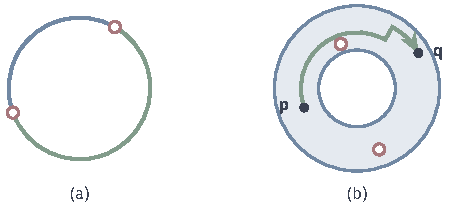
\includegraphics[width=76.962mm]{figures/04-spaces-measures-and-geometry/01-topology-and-metric/tikz/homol-remove-two-points/figure.pdf}
  \caption{圆周与环带各去掉两个点（红色空心点）。(a)圆周断成蓝、绿两段互不相连的开弧。(b)环带中任意两点$\bm p,\bm q$仍可相连：绿色路径先沿圆弧绕到一条避开去掉点的射线，沿射线移动，再沿另一段圆弧到达$\bm q$。}
  \label{fig:homol-remove-two-points}
\end{BookInlineFigure}

从$S^1$中去掉两个不同的点，剩下两段互不相交的开弧，空间不连通。从$A$中去掉任意两点，剩下的部分却仍然路径连通，理由如下。

任取剩下的两点$\bm p,\bm q$。去掉的两点只占两个半径值，所以可以在$\lVert\bm p\rVert_2$附近取一个半径$r_p\in[1,2]$，使半径为$r_p$的圆避开去掉的点，并且从$\bm p$沿半径走到这个圆的短线段也避开它们。对$\bm q$同样取$r_q$。

去掉的点只占两个方向，所以还可以取一条不经过它们的射线。于是从$\bm p$出发沿短线段到半径为$r_p$的圆，沿圆走到射线上，沿射线走到半径为$r_q$的圆，沿这个圆走到$\bm q$的半径方向，最后沿短线段到达$\bm q$。各段首尾相接，就得到一条连接$\bm p,\bm q$的路径。

同胚把“去掉两点”对应为“去掉两点”，并且保持连通性（第~\ref{chap:topological-spaces}章）。两种结果不同，所以$S^1$与$A$不同胚。

可是环带能沿半径连续地压到圆周上，压缩中洞始终存在。要表达“有同样的洞”，需要一种比同胚宽松的比较：不再要求点一一对应，只要求能用连续变形相互转化。下面先定义映射之间的连续变形，再说明怎样把空间连续收回它的子空间。

\subsection{同伦等价}
\label{sec:homol-homotopy-equivalence}

把环带压到圆周上，可以想成一段动画：时间$t$从$0$走到$1$，$t=0$时每个点都在原处，$t=1$时每个点都落到圆周上，中间每一帧都是一个映射。动画要“不跳帧”，不能只要求每一帧连续，还要求同一个点的位置随时间连续变动。

把时间当作一个额外的坐标，这两种连续性就合成了一个条件：动画是定义在“空间$\times$时间”上的一个连续映射。

\begin{definition}[同伦]
\label{def:homol-homotopy}
设$X,Y$为拓扑空间，$f,g:X\to Y$连续，$X\times[0,1]$取乘积拓扑。若存在连续映射$H:X\times[0,1]\to Y$，使得
\begin{equation}
 H(x,0)=f(x),\qquad H(x,1)=g(x),\qquad x\in X,
 \label{eq:homol-homotopy}
\end{equation}
则称$f$与$g$\term{同伦}（homotopy），记为$f\simeq g$，称$H$为从$f$到$g$的一个同伦。
\end{definition}

记$h_t=H(\cdot,t)$，这是动画在时刻$t$的一帧。从图~\ref{fig:homol-homotopy-family}可以同时读出同伦的两种看法：横着看，$X\times[0,1]$的每条水平线给出一个映射$h_t$；竖着看，每条竖线给出一个点$x$的运动轨迹$t\mapsto h_t(x)$。

\begin{BookInlineFigure}
  \centering
  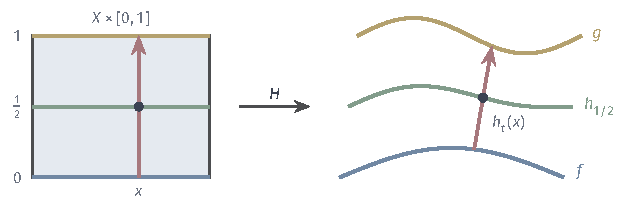
\includegraphics[width=105.971mm]{figures/04-spaces-measures-and-geometry/01-topology-and-metric/tikz/homol-homotopy-family/figure.pdf}
  \caption{同伦把矩形$X\times[0,1]$映到$Y$（此处$X$为线段，$Y$为平面）。蓝、绿、黄三条水平线分别对应$f$、$h_{1/2}$与$g$；红色竖线是固定$x$时的轨迹，它被$H$送成从$f(x)$到$g(x)$的一条路径。}
  \label{fig:homol-homotopy-family}
\end{BookInlineFigure}

$H$在乘积空间上整体连续，比每个$h_t$连续更强。例如令$h_0$为$\mathbb R$上的恒等映射，$t>0$时$h_t$恒取$0$，则每一帧都连续，点$x\neq0$却在$t=0$的瞬间跳到$0$。这样的“跳帧”被整体连续的要求排除了。

最常用的同伦是直线同伦。若$Y\subseteq\mathbb R^n$是凸集，$f,g:X\to Y$连续，令
\begin{equation}
 H(x,t)=(1-t)f(x)+tg(x).
 \label{eq:homol-straight-line-homotopy}
\end{equation}
凸性保证线段上的点仍在$Y$中；$H$由连续函数经乘法与加法得到，因而连续。所以进入凸集的任意两个连续映射都同伦，特别地，进入凸集的映射都同伦于常值映射。

\paragraph{同伦关系的性质}
后面要把同伦的映射看作“同一类”，因此先确认同伦是等价关系，并且与复合相容。

\begin{lemma}[同伦是等价关系]
\label{lem:homol-homotopy-equivalence-relation}
对固定的$X,Y$，连续映射$X\to Y$之间的同伦关系是等价关系。若$f\simeq f':X\to Y$，$g\simeq g':Y\to Z$，则$g\circ f\simeq g'\circ f'$。
\end{lemma}

\begin{proof}
自反性取同伦$H(x,t)=f(x)$，即动画一直停在第一帧。对称性把时间倒过来，若$H$从$f$到$g$，则$H(x,1-t)$从$g$到$f$。

对传递性，设$H$从$f$到$g$，$G$从$g$到$h$。把两段动画接起来，每段用一半时间播放：
\[
 K(x,t)=\begin{cases}H(x,2t),&0\leq t\leq1/2,\\ G(x,2t-1),&1/2\leq t\leq1.\end{cases}
\]
两段在$t=1/2$处都等于$g(x)$，所以$K$有定义。

$K$的连续性用闭集判断。$X\times[0,1/2]$与$X\times[1/2,1]$都是闭集，$K$在其上的限制都连续。对$Y$中任一闭集$F$，$K^{-1}(F)$是两个限制的原像之并。每个原像在相应闭子集中是闭的，因而在整个乘积中是闭的，两个闭集之并仍是闭集，所以$K$连续。

再看与复合的相容性。设$H$从$f$到$f'$，$G$从$g$到$g'$，令
\[
 K(x,t)=G(H(x,t),t).
\]
它是连续映射$(x,t)\mapsto(H(x,t),t)$与$G$的复合，前者的两个分量都连续。代入$t=0$与$t=1$，分别得到$g\circ f$与$g'\circ f'$，所以$K$就是所求的同伦。
\end{proof}

\paragraph{同伦等价与可缩空间}
同胚要求存在互逆的连续映射：去了再回来，恰好回到原处。把“恰好回到原处”放宽为“能连续变回原处”，就得到需要的比较。

\begin{definition}[同伦等价]
\label{def:homol-homotopy-equivalent}
若连续映射$f:X\to Y$与$g:Y\to X$满足
\begin{equation}
 g\circ f\simeq\operatorname{id}_X,\qquad f\circ g\simeq\operatorname{id}_Y,
 \label{eq:homol-homotopy-equivalence}
\end{equation}
则称$f$是\term{同伦等价}（homotopy equivalence），$g$是它的同伦逆，并称$X$与$Y$同伦等价，记为$X\simeq Y$。与单点空间同伦等价的空间称为\term{可缩空间}（contractible space）。
\end{definition}

同胚是同伦等价：互逆映射的复合恰好等于恒等映射。同伦等价的复合仍是同伦等价。设$f:X\to Y$的同伦逆为$g$，$f':Y\to Z$的同伦逆为$g'$，由引理~\ref{lem:homol-homotopy-equivalence-relation}的复合相容性，
\[
 (g\circ g')\circ(f'\circ f)=g\circ(g'\circ f')\circ f
 \simeq g\circ\operatorname{id}_Y\circ f=g\circ f\simeq\operatorname{id}_X,
\]
另一侧同理。所以空间之间的同伦等价也是等价关系。

可缩性有一个更直接的判据：$X$可缩，当且仅当$\operatorname{id}_X$同伦于某个常值映射。设$X\simeq\{p\}$，映射为$f:X\to\{p\}$，同伦逆$g$把$p$送到某点$x_0$，则$g\circ f$是取值$x_0$的常值映射，它同伦于$\operatorname{id}_X$。

反过来，若$\operatorname{id}_X$同伦于取值$x_0$的常值映射，取$f:X\to\{p\}$与$g(p)=x_0$。此时$g\circ f$正是这个常值映射，而$f\circ g=\operatorname{id}_{\{p\}}$自动成立。

\begin{example}[区间与圆盘可缩]
\label{ex:homol-contractible}
闭圆盘是含原点的凸集，记为
\[
 D^2=\{\bm x\in\mathbb R^2:\lVert\bm x\rVert_2\leq1\}.
\]
取直线同伦
\[
 H(\bm x,t)=(1-t)\bm x,
\]
它从恒等映射连续变到取值为原点的常值映射，所以圆盘可缩。例如点$(1,0)$在$t=1/2$时位于$(1/2,0)$，在$t=1$时到达原点。同样的公式把$[-1,1]$收缩到原点。对一般的非空凸集，任取其中一点$\bm a$，用$H(\bm x,t)=(1-t)\bm x+t\bm a$，所以区间$[0,1]$、$\mathbb R^n$及其中任何非空凸集都可缩。
\end{example}

环带是否可缩，直观上似乎一目了然：中间的洞消不掉。但要证明不存在从$\operatorname{id}_A$到常值映射的同伦，就要排除所有可能的连续变形，一个个去试做不到。这正是同调要解决的问题，第~\ref{sec:homol-homotopy-invariance}小节将给出证明。

\paragraph{同伦等价与同胚的区别}
同伦等价比同胚宽松得多。单点与区间$[0,1]$同伦等价，却不同胚，因为两者之间连双射都没有。区间与圆盘都可缩，因而同伦等价，但它们也不同胚。

区间去掉一个内点就不连通。圆盘去掉任何一点$\bm q$却仍然路径连通：任取剩下的两点，取一点$\bm m\in D^2$，使它不在过这两点的直线上；由凸性，两条线段经过$\bm m$把这两点连起来，而除这两点外它们都不在那条直线上，碰不到$\bm q$（$\bm q$若不在这条直线上，直接取线段即可）。同胚把“去掉一点”对应为“去掉一点”，所以二者不同胚。

\begin{BookInlineTable}
  \centering
  \caption{同胚与同伦等价的比较}
  \label{tab:homol-homeo-vs-homotopy}
  \begin{tabular}{lll}
    \toprule
    & 同胚 & 同伦等价 \\
    \midrule
    需要的映射 & 互逆的$f,g$ & 复合同伦于恒等映射的$f,g$ \\
    点的对应 & 一一对应 & 可以把一片压成一点 \\
    保持的信息 & 维数、局部形状等 & 连通分支、洞的个数等 \\
    区间与单点 & 不同 & 相同 \\
    环带与圆周 & 不同 & 相同 \\
    \bottomrule
  \end{tabular}
\end{BookInlineTable}

表~\ref{tab:homol-homeo-vs-homotopy}把两种比较放在一起。同伦等价忽略了维数和点的多少，只保留连续变形下不变的整体信息。表中“保持的信息”一行里的“洞的个数”，还需要用本章后面的同调来说清楚。

\subsection{形变收缩}
\label{sec:homol-deformation-retraction}

环带压向圆周的过程有一个特点：圆周上的点始终不动，其余的点最终都落到圆周上。这样的变形把空间收回到它的一个子空间，而子空间本身不受扰动。

把这个过程拆成两件事：最后的结果是一个把空间收回子空间的映射，过程是把这个映射与恒等映射连起来的同伦。

\begin{definition}[形变收缩]
\label{def:homol-deformation-retraction}
设$Y\subseteq X$为子空间。若连续映射$r:X\to Y$满足$r(a)=a$对一切$a\in Y$成立，则称$r$为\term{回缩}（retraction）。若存在连续映射$H:X\times[0,1]\to X$，满足
\begin{align}
 H(x,0)&=x,\quad H(x,1)\in Y,&x&\in X,\label{eq:homol-deformation-end}\\
 H(a,t)&=a,&a&\in Y,\ t\in[0,1],\label{eq:homol-deformation-fixed}
\end{align}
则称$H$为从$X$到$Y$的\term{形变收缩}（deformation retraction），称$Y$为$X$的形变收缩核。
\end{definition}

两条要求分工不同。式~\eqref{eq:homol-deformation-end}说变形从恒等映射出发，终点落在$Y$中；式~\eqref{eq:homol-deformation-fixed}说$Y$上的点全程固定。两条合起来，终止映射$r=H(\cdot,1)$满足$r|_Y=\operatorname{id}_Y$，是一个回缩；而$H$本身是从$\operatorname{id}_X$到$i\circ r$的同伦，其中$i:Y\to X$是包含映射。

\begin{example}[环带收向圆周]
\label{ex:homol-annulus-retraction}
对环带$A$与圆周$S^1$，令
\begin{equation}
 H(\bm x,t)=(1-t)\bm x+t\frac{\bm x}{\lVert\bm x\rVert_2}.
 \label{eq:homol-annulus-retraction}
\end{equation}
在$A$上$\lVert\bm x\rVert_2\geq1$，分母不为零，所以$H$连续。$H(\bm x,t)$与$\bm x$同方向，长度为
\[
 \lVert H(\bm x,t)\rVert_2=(1-t)\lVert\bm x\rVert_2+t\in[1,2],
\]
所以始终留在$A$中。

$t=0$时$H$是恒等映射。$t=1$时它把每点沿半径送到圆周上，例如点$(0,2)$在$t=1/2$时位于$(0,3/2)$，在$t=1$时到达$(0,1)$。若$\lVert\bm x\rVert_2=1$，则$H(\bm x,t)=\bm x$，圆周上的点不动。因此$H$是从$A$到$S^1$的形变收缩。同一公式也把去掉原点的平面$\mathbb R^2\setminus\{\bm 0\}$形变收缩到$S^1$。
\end{example}

\begin{BookInlineFigure}
  \centering
  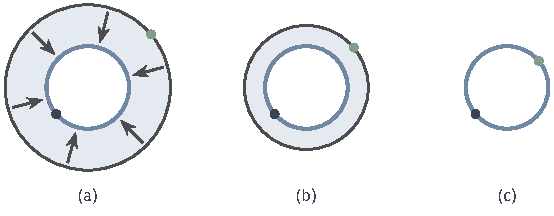
\includegraphics[width=93.832mm]{figures/04-spaces-measures-and-geometry/01-topology-and-metric/tikz/homol-annulus-retraction/figure.pdf}
  \caption{环带沿半径收向圆周，(a)(b)(c)依次是式~\eqref{eq:homol-annulus-retraction}在$t=0,\,1/2,\,1$的像。粗蓝线是单位圆周，全程不动；外缘上的绿点半径由$2$变为$3/2$，再变为$1$；圆周上的黑点始终停在原处。}
  \label{fig:homol-annulus-retraction}
\end{BookInlineFigure}

图~\ref{fig:homol-annulus-retraction}是这个过程的三帧。把它写成一般结论，形变收缩给出的正是同伦等价所需要的那对映射。

\begin{theorem}[形变收缩给出同伦等价]
\label{thm:homol-retract-equivalence}
若$Y$是$X$的形变收缩核，$r=H(\cdot,1)$为相应的回缩，$i:Y\to X$为包含映射，则$i$是同伦等价，$r$是它的同伦逆。特别地，$X\simeq Y$。
\end{theorem}

\begin{proof}
由于$r$在$Y$上是恒等映射，一侧等式严格成立：
\[
 r\circ i=\operatorname{id}_Y.
\]

另一侧，由定义，$H$满足$H(x,0)=x$与$H(x,1)=i(r(x))$，它正是从$\operatorname{id}_X$到$i\circ r$的同伦，所以$i\circ r\simeq\operatorname{id}_X$。
\end{proof}

由例~\ref{ex:homol-annulus-retraction}与定理~\ref{thm:homol-retract-equivalence}，$A\simeq S^1$。环带与圆周不同胚，却同伦等价，这正是本节开头想表达的“有同样的洞”。

\paragraph{回缩本身不够}
只有回缩而没有形变，不能得出同伦等价。取两点离散空间$X=\{0,1\}$与子空间$Y=\{0\}$，常值映射$r\equiv0$是回缩。若$i\circ r\simeq\operatorname{id}_X$，同伦限制在点$1$上就给出一条从$0$到$1$的路径，可是$X$不连通，这样的路径不存在。

所以$Y$不是$X$的形变收缩核。回缩只说“结果”：每个点都有去处。形变收缩还要求“过程”：每个点能沿连续的路径走到去处。上面的点$1$有去处，却没有路可走。

定义要求$Y$全程固定，这比同伦等价所需要的略强。若只要$X\simeq Y$，允许$Y$中的点在$Y$内部移动也够了：此时$H$限制在$Y$上给出$r\circ i\simeq\operatorname{id}_Y$，定理~\ref{thm:homol-retract-equivalence}的结论不变。保留固定条件，是因为它描述的正是“把多余部分收回、核心不动”这一具体过程；第~\ref{chap:manifold-recovery}章把点云邻域收回流形时，用的就是这种形式。

同伦等价究竟保留了什么代数信息，需要先建立同调才能回答。下一节先解决输入的问题：怎样把一个空间写成有限的数据。

\section{有限单纯复形}
\label{sec:homol-simplicial-complexes}

要计算洞，先要有能写成有限数据的空间。图是一个候选：它用顶点和边记录直接连接，也可以有环（可参考\BookChapterRef{chap:graph-objects}{卷三第1章“图与连接结构”}）。但本章开头的三角形框与三角形纸片有同一张图，三个顶点两两相邻。图中的环$0\to1\to2\to0$在框上围着一个洞，在纸片上却什么也没围住。

只记录邻接边，就丢掉了“这个环已经被填上”的信息。修补的办法是把“填充”也记下来：除了点和边，还允许记录三个顶点张成的三角形、四个顶点张成的四面体，等等。本节先建立这种有限的组合对象，再把它实现为欧氏空间中的子集，使连续映射与同伦能够作用在它上面。

\subsection{单纯复形的定义}
\label{sec:homol-complex-definition}

一个填充三角形由它的三个顶点确定，一条边由两个端点确定，所以一块“填充”可以简单地记为一个顶点子集。记录要前后一致：填入一个三角形时，它的三条边和三个顶点也必须在记录之中，否则三角形的边缘无处安放。

\begin{definition}[抽象单纯复形]
\label{def:homol-simplicial-complex}
设$V$为有限集。由$V$的非空子集组成的族$\mathcal K$称为以$V$为顶点集的\term{抽象单纯复形}（abstract simplicial complex），若
\begin{itemize}
 \item 对每个$v\in V$，$\{v\}\in\mathcal K$；
 \item 若$\sigma\in\mathcal K$且$\varnothing\neq\tau\subseteq\sigma$，则$\tau\in\mathcal K$。
\end{itemize}
$\mathcal K$中的元素称为\term{单纯形}（simplex）。含$k+1$个顶点的单纯形称为$k$维单纯形，简称$k$-单纯形；单纯形$\sigma$的非空子集称为它的\term{面}（face）。$\mathcal K$中单纯形维数的最大值称为$\mathcal K$的维数。
\end{definition}

第二条要求称为对取面封闭，它正是上面所说的“填入三角形时，边和顶点也要在”。$0$维单纯形是顶点，$1$维单纯形是边，$2$维单纯形是填充三角形，$3$维单纯形是实心四面体。

一维的单纯复形恰好就是一张简单无向图：顶点集是$V$，边集是二元单纯形的全体。单纯复形因而可以看作图向高维的推广。

记$n_k$为$\mathcal K$中$k$维单纯形的个数。若$\mathcal L\subseteq\mathcal K$本身也是单纯复形，就称$\mathcal L$为$\mathcal K$的\term{子复形}（subcomplex）。维数不超过$k$的单纯形组成的子复形称为$\mathcal K$的$k$维\term{骨架}（skeleton），记为$\mathcal K^{(k)}$；一维骨架就是$\mathcal K$的顶点与边组成的图。

\begin{example}[三角形边界与填实三角形]
\label{ex:homol-two-triangles}
取$V=\{0,1,2\}$，令
\begin{align*}
 \mathcal T_1&=\bigl\{\{0\},\{1\},\{2\},\{0,1\},\{1,2\},\{0,2\}\bigr\},\\
 \mathcal T_2&=\mathcal T_1\cup\bigl\{\{0,1,2\}\bigr\}.
\end{align*}
两者都对取面封闭。$\mathcal T_1$是一维复形，单纯形个数为$(n_0,n_1)=(3,3)$，记录三角形的边界；$\mathcal T_2$是二维复形，单纯形个数为$(n_0,n_1,n_2)=(3,3,1)$，记录填实的三角形。

它们的一维骨架相同，都是三个顶点两两相邻的图，$\mathcal T_1$是$\mathcal T_2$的子复形。集合族$\bigl\{\{0\},\{1\},\{2\},\{0,1,2\}\bigr\}$则不是单纯复形，它记录了三角形，却缺少三条边。
\end{example}

图~\ref{fig:homol-triangle-complexes}的前三幅画出了这三个集合族。比较(a)与(b)，例~\ref{ex:homol-two-triangles}说明图中的环未必对应复形中的洞：在$\mathcal T_2$中，环$0\to1\to2\to0$恰好是那个填充三角形的边界。判断一个环是否围住了洞，要看它能否被某些高维单纯形“填掉”，第~\ref{sec:homol-simplicial-homology}节用边界映射把这件事说精确。

\begin{BookInlineFigure}
  \centering
  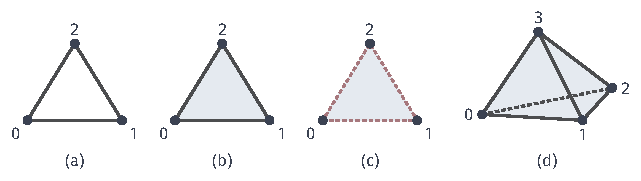
\includegraphics[width=108.532mm]{figures/04-spaces-measures-and-geometry/01-topology-and-metric/tikz/homol-triangle-complexes/figure.pdf}
  \caption{有限单纯复形及一个反例。(a)$\mathcal T_1$：三角形边界。(b)$\mathcal T_2$：填实的三角形，比(a)多一个二维单纯形（浅蓝）。(c)只有填充和顶点、没有三条边的集合族（红色虚线表示缺失的边），不对取面封闭。(d)$\mathcal S$：空心四面体表面，虚线是被遮挡的边，内部没有三维单纯形。}
  \label{fig:homol-triangle-complexes}
\end{BookInlineFigure}

\begin{example}[四面体的表面]
\label{ex:homol-tetrahedron-boundary}
取$V=\{0,1,2,3\}$，令$\mathcal S$由$V$的全部非空真子集组成，即$4$个顶点、$6$条边和$4$个三角形，单纯形个数为$(n_0,n_1,n_2)=(4,6,4)$，不含$3$维单纯形$\{0,1,2,3\}$。它记录空心四面体的表面，见图~\ref{fig:homol-triangle-complexes}(d)，中间围住一个“二维的洞”。再加上$V$本身，就得到实心四面体。
\end{example}

\subsection{几何实现}
\label{sec:homol-geometric-realization}

抽象单纯复形只是集合族，没有点、开集或连续映射。要谈论同伦，必须把它变成一个拓扑空间：每个$k$维单纯形换成一块$k$维的“实心”几何对象，再把公共的面粘在一起。

\paragraph{标准单纯形}
先定下这块几何对象。在$\mathbb R^{k+1}$中，取坐标非负且和为$1$的点，得到
\begin{equation}
 \Delta^k=\Bigl\{\bm t=(t_0,\ldots,t_k)\in\mathbb R^{k+1}:t_i\geq0,\ \sum_{i=0}^kt_i=1\Bigr\},
 \label{eq:homol-standard-simplex}
\end{equation}
称为$k$维\term{标准单纯形}（standard simplex），取$\mathbb R^{k+1}$的子空间拓扑。它是标准基向量$\bm e_0,\ldots,\bm e_k$的凸包，有界且闭，因而紧。

$\Delta^0$是一点，$\Delta^1$是线段，$\Delta^2$是三角形，$\Delta^3$是四面体，图~\ref{fig:homol-standard-simplices}画出了后三者。坐标$t_i$可以读成“$\bm e_i$的权重”：$\Delta^2$中的点$\bm t=(\frac12,\frac14,\frac14)$就是
\[
 \tfrac12\bm e_0+\tfrac14\bm e_1+\tfrac14\bm e_2,
\]
三个顶点的加权平均。把某些坐标取为零，得到的子集仍是由其余基向量张成的低维单纯形，称为$\Delta^k$的面。例如$\Delta^2$中$t_0=0$的点组成连接$\bm e_1,\bm e_2$的边。

\begin{BookInlineFigure}
  \centering
  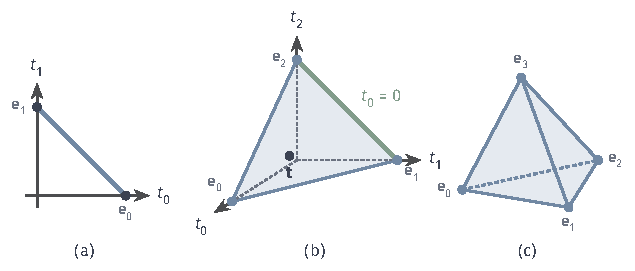
\includegraphics[width=107.453mm]{figures/04-spaces-measures-and-geometry/01-topology-and-metric/tikz/homol-standard-simplices/figure.pdf}
  \caption{标准单纯形。(a)$\Delta^1$是$\mathbb R^2$中连接$\bm e_0,\bm e_1$的线段。(b)$\Delta^2$是$\mathbb R^3$中的三角形，黑点是$\bm t=(\frac12,\frac14,\frac14)$；绿色边是$t_0=0$的面。(c)$\Delta^3$位于$\mathbb R^4$中，此处按四面体形状示意，虚线是被遮挡的边。}
  \label{fig:homol-standard-simplices}
\end{BookInlineFigure}

\paragraph{沿公共面粘合}
下面把单纯形按记录粘起来。设$\mathcal K$的顶点集为$V$。对每个单纯形$\sigma\in\mathcal K$，取一份以$\sigma$的顶点为坐标编号的几何单纯形：
\[
 \Delta^\sigma=\Bigl\{(t_v)_{v\in\sigma}:t_v\geq0,\ \sum_{v\in\sigma}t_v=1\Bigr\}.
\]

把各份放在某个欧氏空间中互不相交的位置，它们的并记为$W$，取子空间拓扑。$W$是有限个紧集之并，因而紧。若$\tau\subseteq\sigma$，则$\Delta^\tau$可以看作$\Delta^\sigma$中$\sigma\setminus\tau$各坐标为零的那个面。

在$W$上规定：$\Delta^\tau$中的点与$\Delta^\sigma$中对应面上坐标相同的点等价，并取由此生成的等价关系$\sim$。商空间$W/{\sim}$（第~\ref{chap:topological-spaces}章）就是把每个面与它在复形中对应的单纯形粘成一份，图~\ref{fig:homol-gluing}(a)(b)画的是两个三角形沿公共边粘合的情形。

\begin{BookInlineFigure}
  \centering
  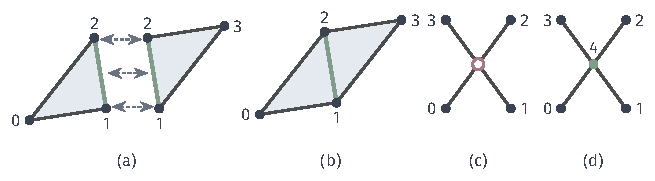
\includegraphics[width=110.973mm]{figures/04-spaces-measures-and-geometry/01-topology-and-metric/tikz/homol-gluing/figure.pdf}
  \caption{粘合与画法。(a)$\{0,1,2\}$与$\{1,2,3\}$的两份几何单纯形，公共边的两份副本为绿色，虚线箭头连接被等同的点。(b)粘合结果。(c)边$\{0,2\}$与$\{1,3\}$在纸上交叉，但红色空心点不是复形中的点。(d)加入新顶点$4$并把两条边各拆成两段之后，四条边才在$4$相遇。}
  \label{fig:homol-gluing}
\end{BookInlineFigure}

这个商空间可以直接放进欧氏空间。把顶点集写成$V=\{v_1,\ldots,v_n\}$，在$\mathbb R^n$中令顶点$v_j$对应标准基向量$\bm e_j$，记
\begin{equation}
 \lvert\mathcal K\rvert=\bigcup_{\sigma\in\mathcal K}\operatorname{conv}\{\bm e_j:v_j\in\sigma\}\subseteq\mathbb R^n,
 \label{eq:homol-realization}
\end{equation}
取子空间拓扑，其中$\operatorname{conv}$表示凸包。

$\lvert\mathcal K\rvert$中的点$\bm x=\sum_jx_j\bm e_j$满足$x_j\geq0$、$\sum_jx_j=1$，这些坐标称为\term{重心坐标}（barycentric coordinates），坐标为正的顶点组成的集合称为它的支撑。重心坐标告诉我们这个点是哪些顶点的加权平均，支撑告诉我们它落在哪一块单纯形的“内部”。

\begin{lemma}[几何单纯形只在公共面上相交]
\label{lem:homol-simplices-intersect}
在式~\eqref{eq:homol-realization}中，点$\bm x$属于$\sigma$对应的凸包，当且仅当它的支撑包含于$\sigma$。因此$\sigma,\tau$对应的两个凸包之交恰为$\sigma\cap\tau$对应的凸包；当$\sigma\cap\tau=\varnothing$时，二者不相交。每个点的支撑本身是$\mathcal K$中的一个单纯形。
\end{lemma}

\begin{proof}
$\sigma$对应的凸包由非负、和为一、且在$\sigma$以外的坐标为零的向量组成，所以$\bm x$属于它当且仅当支撑包含于$\sigma$。

两个凸包都含$\bm x$，当且仅当支撑同时包含于$\sigma$与$\tau$，即包含于$\sigma\cap\tau$，这恰好是$\bm x$属于$\sigma\cap\tau$对应的凸包。

若$\bm x$属于某个$\sigma$对应的凸包，它的支撑是$\sigma$的非空子集，由取面封闭性仍属于$\mathcal K$。
\end{proof}

现在比较商空间$W/{\sim}$与$\lvert\mathcal K\rvert$。把$\Delta^\sigma$中的点$(t_v)_{v\in\sigma}$送到$\sum_{v_j\in\sigma}t_{v_j}\bm e_j$，得到连续满射$\Phi:W\to\lvert\mathcal K\rvert$。

两点被$\Phi$送到同一点，当且仅当它们有相同的非零坐标。记这些坐标所在的顶点集为$\rho$，由引理~\ref{lem:homol-simplices-intersect}它是一个单纯形，两点都是$\Delta^\rho$中同一点在各自单纯形的面上的副本，恰好被$\sim$等同。所以$\Phi$诱导出连续双射
\[
 \bar\Phi:W/{\sim}\to\lvert\mathcal K\rvert.
\]

要说明$\bar\Phi$是同胚，还需要逆映射连续。下面的引理把这一步化成紧性，这也是拓扑中判定同胚最常用的手段。

\begin{lemma}[紧空间到Hausdorff空间的连续双射]
\label{lem:homol-compact-hausdorff}
设$X$紧，$Y$是Hausdorff空间，$f:X\to Y$是连续双射，则$f$是同胚。
\end{lemma}

\begin{proof}
只需证明$f$把闭集映为闭集，这样$f^{-1}$作用下闭集的原像是闭集，$f^{-1}$连续。

设$F\subseteq X$闭。紧空间的闭子集是紧的，紧集的连续像是紧的，所以$f(F)$紧。

还要说明Hausdorff空间中的紧集$C$是闭集。任取$y\notin C$，对每个$c\in C$取$y$的邻域$U_c$与$c$的邻域$V_c$使二者不交。各$V_c$覆盖$C$，由紧性有有限子覆盖；相应有限个$U_c$之交是$y$的邻域，它与$C$不交。所以$C$的补集是开集，$f(F)$是闭集。
\end{proof}

$W$紧，商映射连续，所以$W/{\sim}$紧。$\lvert\mathcal K\rvert$是欧氏空间的子集，是Hausdorff空间。由引理~\ref{lem:homol-compact-hausdorff}，$\bar\Phi$是同胚。我们把$\lvert\mathcal K\rvert$称为$\mathcal K$的\term{几何实现}（geometric realization）。若拓扑空间$X$同胚于某个$\lvert\mathcal K\rvert$，就称$\mathcal K$是$X$的一个\term{三角剖分}（triangulation）。

\paragraph{抽象顶点、坐标与空间}
几何实现涉及三个层次，不能混淆。抽象顶点只是$V$中的名字。坐标表示是选定的嵌入，例如式~\eqref{eq:homol-realization}用标准基向量，也可以用平面上的三个点实现$\mathcal T_2$。空间本身则是同胚意义下确定的对象。

换一种坐标表示，只要每个单纯形实现为相应顶点的凸包，且不同单纯形只在公共面上相交，得到的空间就与$\lvert\mathcal K\rvert$同胚，理由与上面相同。这与线性代数中“向量本身与它的坐标”的区别是同一回事：选坐标是为了计算，选法不影响对象。

\begin{example}[三角形边界是圆周]
\label{ex:homol-triangle-circle}
把$\mathcal T_1$的三个顶点实现为平面上一个三角形的三个顶点，三条边实现为三条边线，得到三角形边线$T\subseteq\mathbb R^2$。取三角形的重心$\bm c$，考虑径向投影
\[
 \bm x\mapsto\frac{\bm x-\bm c}{\lVert\bm x-\bm c\rVert_2},\qquad T\to S^1.
\]
从$\bm c$出发的每条射线恰好与$T$交于一点，所以这是连续双射。$T$紧，$S^1$是Hausdorff空间，由引理~\ref{lem:homol-compact-hausdorff}，它是同胚，所以$\lvert\mathcal T_1\rvert\cong S^1$。

对填实的三角形，沿每条从$\bm c$出发的射线做线性伸缩，把射线上落在三角形内的线段拉成单位长度。三角形写成三个半平面$\langle\bm n_e,\bm x-\bm c\rangle\leq d_e$（$d_e>0$）的交，令
\[
 p(\bm v)=\max_e\frac{\langle\bm n_e,\bm v\rangle}{d_e},
\]
这样$\bm x$在三角形内当且仅当$p(\bm x-\bm c)\leq1$，$p$是连续函数。令$G(\bm c)=\bm 0$，其余点令
\[
 G(\bm x)=p(\bm x-\bm c)\,\frac{\bm x-\bm c}{\lVert\bm x-\bm c\rVert_2}.
\]
$G$是从三角形到$D^2$的连续双射，再由引理~\ref{lem:homol-compact-hausdorff}得$\lvert\mathcal T_2\rvert\cong D^2$。同样的径向投影给出$\lvert\mathcal S\rvert\cong S^2$。
\end{example}

画在纸上的图形却可能误导。取$V=\{0,1,2,3\}$与
\[
 \mathcal K=\bigl\{\{0\},\{1\},\{2\},\{3\},\{0,2\},\{1,3\}\bigr\},
\]
把四个顶点画在正方形的四角，两条边画成两条对角线，纸上的线段在中心交叉，如图~\ref{fig:homol-gluing}(c)所示。

由引理~\ref{lem:homol-simplices-intersect}，$\{0,2\}$与$\{1,3\}$不交，它们的实现在$\mathbb R^4$中也不相交：$\lvert\mathcal K\rvert$是两条互不相交的线段，而不是一个“X”形。画法中的交叉点不是复形中的点。要表示两条边在中间相遇，必须在复形中加入一个新顶点，并把两条边各拆成两段，如图~\ref{fig:homol-gluing}(d)所示。

\section{单纯同调}
\label{sec:homol-simplicial-homology}

在$\mathcal T_1$与$\mathcal T_2$中，环$0\to1\to2\to0$都是“闭合”的：沿它走一圈回到起点，没有多余的端点。区别在于，$\mathcal T_2$中这个环恰好是填充三角形的边界，而$\mathcal T_1$中没有任何二维单纯形以它为边界。要把这个区别变成可计算的量，需要能把若干条边“相加”成一个环，并对一个单纯形“取边界”。

本节固定实数系数，把同维单纯形的有限线性组合组成向量空间，称为链；边界映射是链空间之间的线性映射。闭合的链是边界映射的核，已被填掉的链是高一维边界映射的像，同调就是二者之商。这样，有限复形的孔洞计算全部归结为矩阵的核、像与秩，所用的结论（核与像是子空间、秩零度定理、商空间及其维数）可参考\BookChapterRef{chap:linear-representation}{卷二第2章“线性空间、映射与坐标”}。

\subsection{边界映射}
\label{sec:homol-boundary-map}

线段的边界是两个端点，但要让“闭合”表现为“边界为零”，端点必须带符号：从$0$走到$1$，记作“终点减起点”$1-0$；再从$1$走回$0$，记作$0-1$，两者相加为零。所以先给每个单纯形规定方向，再定义带符号的边界。

\paragraph{定向与链空间}
把$k$-单纯形$\sigma=\{v_0,\ldots,v_k\}$的顶点排成一个次序，记为$[v_0,\ldots,v_k]$，称为一个有向单纯形。同一单纯形的不同排列之间规定
\begin{equation}
 [v_{\pi(0)},\ldots,v_{\pi(k)}]=\operatorname{sgn}(\pi)\,[v_0,\ldots,v_k],
 \label{eq:homol-orientation-sign}
\end{equation}
其中$\pi$是$\{0,\ldots,k\}$的置换，$\operatorname{sgn}(\pi)$是它的符号。于是交换两个顶点改变符号，偶置换不改变它。$k\geq1$时一个单纯形恰有两种\term{定向}（orientation），彼此相差一个负号；顶点只有一种。

\begin{definition}[链空间]
\label{def:homol-chain-space}
固定$V$上的一个全序，对每个$k$-单纯形取顶点递增排列的有向单纯形。以这$n_k$个有向单纯形为基的实向量空间记为$C_k(\mathcal K)$，称为$k$维\term{链空间}（chain space），其元素称为$k$维链。$k<0$或$k$大于$\mathcal K$的维数时，规定$C_k(\mathcal K)=0$。
\end{definition}

一个$k$维链形如$\bm c=\sum_\sigma c_\sigma\sigma$，其中求和遍历$k$-单纯形，$c_\sigma\in\mathbb R$，因而$C_k(\mathcal K)\cong\mathbb R^{n_k}$。任意排列的有向单纯形都按式~\eqref{eq:homol-orientation-sign}化为基向量的$\pm1$倍，所以选哪个全序只影响基向量的符号，不影响链空间本身。系数可以是任意实数，例如$2[0,1]$表示把这条边走两遍，$-[0,1]=[1,0]$表示反向走一遍。

\paragraph{边界映射的定义}
$k$-单纯形的边界由它的$k+1$个$(k-1)$维面组成；依次去掉第$i$个顶点，并用符号$(-1)^i$交错相加。

\begin{definition}[边界映射]
\label{def:homol-boundary-map}
对$k\geq1$，在有向单纯形上令
\begin{equation}
 \partial_k[v_0,\ldots,v_k]=\sum_{i=0}^k(-1)^i[v_0,\ldots,\widehat{v_i},\ldots,v_k],
 \label{eq:homol-boundary}
\end{equation}
其中$\widehat{v_i}$表示去掉$v_i$，并线性延拓为$\partial_k:C_k(\mathcal K)\to C_{k-1}(\mathcal K)$。规定$\partial_0=0$。$\partial_k$称为\term{边界映射}（boundary map）。
\end{definition}

低维情形最直观。$\partial_1[v_0,v_1]=v_1-v_0$，即终点减起点；$\partial_2[v_0,v_1,v_2]=[v_1,v_2]-[v_0,v_2]+[v_0,v_1]=[v_0,v_1]+[v_1,v_2]+[v_2,v_0]$，是沿三角形绕行一周的三条有向边。

式~\eqref{eq:homol-boundary}对每一种排列给出一个值，必须检查它与式~\eqref{eq:homol-orientation-sign}相容，即交换顶点次序时右端也改变符号。由于任意置换都是相邻对换的复合，只需检查交换$v_j$与$v_{j+1}$。对$i\notin\{j,j+1\}$，第$i$项的面中这两个顶点仍相邻且被交换，按式~\eqref{eq:homol-orientation-sign}改变符号，而系数$(-1)^i$不变。$i=j$与$i=j+1$两项则互换：交换后去掉第$j$个位置得到的是原来去掉$v_{j+1}$的面，系数由$(-1)^{j+1}$变为$(-1)^j$，另一项同理。所以整个右端变为相反数，$\partial_k$是良好定义的线性映射。

\paragraph{边界矩阵}
在定义~\ref{def:homol-chain-space}的基下，$\partial_k$由一个$n_{k-1}\times n_k$矩阵$\bm D_k$表示，第$\sigma$列记录$\partial_k\sigma$的系数，每列恰有$k+1$个$\pm1$。

\begin{example}[两个三角形的边界矩阵]
\label{ex:homol-boundary-matrices}
在$\mathcal T_1$中按$0<1<2$定向，边的基取$a=[0,1]$、$b=[1,2]$、$c=[0,2]$。由$\partial_1a=1-0$、$\partial_1b=2-1$、$\partial_1c=2-0$，按顶点$0,1,2$排行、按$a,b,c$排列，得到
\[
 \bm D_1=\begin{bmatrix}-1&0&-1\\1&-1&0\\0&1&1\end{bmatrix}.
\]
$\mathcal T_2$还有一个二维单纯形$s=[0,1,2]$，$\partial_2s=b-c+a$，所以$\bm D_2=(1,1,-1)^\top$。直接相乘，$\bm D_1\bm D_2$的三个分量依次为$-1+0+1$、$1-1+0$、$0+1-1$，全为零。
\end{example}

$\bm D_1$的每一列在起点处为$-1$、终点处为$1$。卷三定义的关联矩阵按记录方向在起点处记$1$、终点处记$-1$，所以在相同的边方向下，$\bm D_1$恰为关联矩阵的相反数。一维边界映射只是带符号地记录了图的连接，二维以上的边界矩阵才记录填充。

\paragraph{两次取边界为零}
例~\ref{ex:homol-boundary-matrices}中$\bm D_1\bm D_2=\bm 0$不是巧合：三角形边界绕行一周回到起点，端点的贡献正负相消。这个现象对一切维数成立。

\begin{theorem}[边界的边界为零]
\label{thm:homol-boundary-squared}
对一切$k$，$\partial_{k-1}\circ\partial_k=0$。
\end{theorem}

\begin{proof}
由线性性，只需对有向单纯形$[v_0,\ldots,v_k]$验证。展开两次边界，每一项都是去掉两个顶点$v_a,v_b$（$a<b$）得到的$(k-2)$维面，并且恰好出现两次。先去掉$v_b$，它位于第$b$个位置，系数为$(-1)^b$；此时$v_a$仍位于第$a$个位置，再去掉它，系数为$(-1)^a$。先去掉$v_a$，系数为$(-1)^a$；此时$v_b$前移到第$b-1$个位置，再去掉它，系数为$(-1)^{b-1}$。两项系数分别为$(-1)^{a+b}$与$(-1)^{a+b-1}$，互为相反数，全部相消。
\end{proof}

满足$\partial_{k-1}\circ\partial_k=0$的一列向量空间与线性映射
\[
 \cdots\xrightarrow{\ \partial_{k+1}\ }C_k(\mathcal K)\xrightarrow{\ \partial_k\ }C_{k-1}(\mathcal K)\xrightarrow{\ \partial_{k-1}\ }\cdots\xrightarrow{\ \partial_1\ }C_0(\mathcal K)\xrightarrow{\ \partial_0\ }0
\]
称为\term{链复形}（chain complex）。定理~\ref{thm:homol-boundary-squared}说明，任何链的边界都是“闭合”的；下一小节把这一点写成子空间的包含关系。

\subsection{同调空间}
\label{sec:homol-homology-spaces}

边界为零的链没有多余的端点，是闭合的；某个高一维链的边界，则是已经被填掉的。定理~\ref{thm:homol-boundary-squared}说后者总是前者的一部分。“没有被填掉的闭合结构”，就是从前者中除去后者剩下的部分。

\begin{definition}[闭链、边界链与同调空间]
\label{def:homol-homology}
令
\[
 Z_k(\mathcal K)=\ker\partial_k,\qquad B_k(\mathcal K)=\operatorname{im}\partial_{k+1},
\]
其元素分别称为$k$维\term{闭链}（cycle）与$k$维\term{边界链}（boundary chain）。由定理~\ref{thm:homol-boundary-squared}，$B_k(\mathcal K)\subseteq Z_k(\mathcal K)$。商空间
\[
 H_k(\mathcal K)=Z_k(\mathcal K)/B_k(\mathcal K)
\]
称为$\mathcal K$的$k$维（实系数）单纯\term{同调空间}（homology space），其维数$\beta_k=\dim H_k(\mathcal K)$称为第$k$个\term{Betti数}（Betti number）。
\end{definition}

闭链$\bm z$所在的类$\bm z+B_k(\mathcal K)$记为$[\bm z]$，称为它的同调类。两个闭链同调，即$[\bm z]=[\bm z']$，当且仅当$\bm z-\bm z'$是某个$(k+1)$维链的边界，也就是二者相差一块被填充的部分。$[\bm z]=0$表示$\bm z$本身已被填掉。

由商空间的维数公式与秩零度定理，$\dim Z_k=n_k-\operatorname{rank}\bm D_k$，$\dim B_k=\operatorname{rank}\bm D_{k+1}$，所以
\begin{equation}
 \beta_k=n_k-\operatorname{rank}\bm D_k-\operatorname{rank}\bm D_{k+1}.
 \label{eq:homol-betti-rank}
\end{equation}
有限复形的Betti数只需数单纯形、求边界矩阵的秩。$\bm D_0$与维数以上的$\bm D_k$都按零矩阵处理。

\begin{example}[三角形边界与填实三角形的同调]
\label{ex:homol-triangle-homology}
沿用例~\ref{ex:homol-boundary-matrices}。$\bm D_1$的第三列等于前两列之和，前两列线性无关，所以$\operatorname{rank}\bm D_1=2$。解$\bm D_1\bm x=\bm0$得$x_a=x_b=-x_c$，于是
\[
 Z_1(\mathcal T_1)=Z_1(\mathcal T_2)=\operatorname{span}\{\bm z\},\qquad\bm z=a+b-c=[0,1]+[1,2]+[2,0].
\]
对$\mathcal T_1$，没有二维单纯形，$B_1=0$，由式~\eqref{eq:homol-betti-rank}，$\beta_1=3-2-0=1$，$H_1(\mathcal T_1)$由$[\bm z]$张成。对$\mathcal T_2$，$\partial_2s=\bm z$，$B_1=Z_1$，$\beta_1=3-2-1=0$；又$\bm D_2\neq\bm 0$，$\ker\partial_2=0$，$\beta_2=0$。两者都有$\beta_0=3-0-2=1$。
\end{example}

例~\ref{ex:homol-triangle-homology}把本章开头的区别变成了一个数：两个复形的一维骨架相同，闭链空间也相同，差别全在$B_1$中。框上的环是闭链而非边界，$\beta_1=1$；纸片上的同一个环是填充三角形的边界，$\beta_1=0$。

\paragraph{零维同调与连通分量}
$\beta_0$在两个例子中都是$1$，对应“只有一块”。这不是巧合。

\begin{theorem}[零维同调计数连通分量]
\label{thm:homol-h0-components}
设$\mathcal K$的一维骨架作为图有连通分量$C_1,\ldots,C_m$，从每个分量中各取一个顶点$u_j$。则$[u_1],\ldots,[u_m]$是$H_0(\mathcal K)$的一组基，特别地，$\beta_0$等于连通分量的个数。
\end{theorem}

\begin{proof}
由$\partial_0=0$，$Z_0=C_0(\mathcal K)$，$B_0$由所有边的边界$v-u$张成。若$v$与$u_j$在同一分量中，取一条路径$u_j=w_0,w_1,\ldots,w_\ell=v$，则$v-u_j=\sum_i(w_{i+1}-w_i)$是各边边界之和（反向边差一个符号），所以$[v]=[u_j]$。于是每个顶点的类都是某个$[u_j]$，$[u_1],\ldots,[u_m]$张成$H_0$。

再证线性无关。对每个分量$C_j$，定义线性函数$\varphi_j(\bm c)=\sum_{v\in C_j}c_v$，即$\bm c$在$C_j$中各顶点上系数之和。每条边的两个端点在同一分量中，所以$\varphi_j(v-u)=0$，$\varphi_j$在$B_0$上为零，因而在$H_0$上有定义。若$\sum_j\lambda_j[u_j]=0$，用$\varphi_l$作用得$\lambda_l=0$。
\end{proof}

由此也得到$\operatorname{rank}\bm D_1=n_0-m$。在例~\ref{ex:homol-triangle-homology}中，$m=1$，$\operatorname{rank}\bm D_1=3-1=2$，与直接计算一致。

\paragraph{二维的洞}
同样的计算在高维记录被围住的空腔。

\begin{example}[四面体表面的同调]
\label{ex:homol-tetrahedron-homology}
对例~\ref{ex:homol-tetrahedron-boundary}的$\mathcal S$，记去掉顶点$i$的三角形为$f_i$（顶点递增排列）。按式~\eqref{eq:homol-boundary}对四个顶点的有向单纯形形式地取边界，得到
\[
 \bm w=f_0-f_1+f_2-f_3;
\]
由定理~\ref{thm:homol-boundary-squared}的同一计算，$\partial_2\bm w=0$，所以$\bm w$是二维闭链。反过来，设$\sum_ic_if_i\in\ker\partial_2$。任意两个三角形恰好共有一条边，而每条边恰好属于两个三角形，所以这条边的系数为$c_i\pm c_j=0$，各$c_i$都由$c_0$确定，$\dim Z_2\leq1$。于是$Z_2=\operatorname{span}\{\bm w\}$，$\mathcal S$中没有三维单纯形，$\beta_2=1$，$\operatorname{rank}\bm D_2=4-1=3$。

一维骨架是四个顶点两两相邻的连通图，由定理~\ref{thm:homol-h0-components}，$\beta_0=1$，$\operatorname{rank}\bm D_1=3$。由式~\eqref{eq:homol-betti-rank}，$\beta_1=6-3-3=0$。空心四面体表面上的每个闭合环都能用表面上的三角形填掉，但整个表面围住了一个空腔。加入$\{0,1,2,3\}$后，$\bm w$成为它的边界，$\beta_2$变为$0$。
\end{example}

\paragraph{用单纯形个数核对Betti数}
Betti数各自要求秩，但它们的交错和只依赖单纯形的个数，可以用来核对手算。

\begin{theorem}[Euler示性数]
\label{thm:homol-euler-characteristic}
设$\mathcal K$的维数为$d$，则
\[
 \sum_{k=0}^d(-1)^kn_k=\sum_{k=0}^d(-1)^k\beta_k.
\]
左端称为$\mathcal K$的\term{Euler示性数}（Euler characteristic），记为$\chi(\mathcal K)$。
\end{theorem}

\begin{proof}
对$\partial_k:C_k\to C_{k-1}$用秩零度定理，$n_k=\dim Z_k+\operatorname{rank}\bm D_k$；又$\beta_k=\dim Z_k-\operatorname{rank}\bm D_{k+1}$。两式相减得$n_k-\beta_k=\operatorname{rank}\bm D_k+\operatorname{rank}\bm D_{k+1}$。乘以$(-1)^k$对$k=0,\ldots,d$求和，相邻两项的$\operatorname{rank}\bm D_{k+1}$以相反符号出现而相消，剩下$\operatorname{rank}\bm D_0$与$\operatorname{rank}\bm D_{d+1}$，二者都为零。
\end{proof}

核对：$\chi(\mathcal T_1)=3-3=0=1-1$，$\chi(\mathcal T_2)=3-3+1=1=1-0+0$，$\chi(\mathcal S)=4-6+4=2=1-0+1$。反过来，已知其余Betti数时，Euler示性数可以省去一次求秩。

\paragraph{同调记录了什么，没有记录什么}
$\beta_0$计数连通分量，$\beta_1$计数没有被填掉的独立环，$\beta_2$计数被围住的空腔。“独立”是线性代数意义上的：在$\mathcal T_1$上把$\bm z$走两遍得到$2\bm z$，它与$\bm z$属于同一条直线，不算新的洞。

同调相同不足以判定空间同胚。单点复形$\{\{0\}\}$与$\mathcal T_2$的Betti数都是$(1,0,0,\ldots)$，但单点与圆盘之间没有双射。$\mathcal T_2$与只有一条边的复形$\bigl\{\{0\},\{1\},\{0,1\}\bigr\}$也有相同的Betti数，而圆盘与线段不同胚（第~\ref{sec:homol-homotopy-equivalence}小节）。同调只记录连通与孔洞的数目，不记录维数与精细形状。实数系数还会忽略一部分只在整数系数下才能看到的信息，这里不展开。

\subsection{包含诱导的同调映射}
\label{sec:homol-induced-inclusion}

在$\mathcal T_1$上填入三角形得到$\mathcal T_2$，$\beta_1$从$1$变为$0$。我们想说的不只是“数从$1$变成$0$”，而是“原来那个环被填掉了”。为此需要把小复形的同调类送进大复形，看它变成了什么。

\paragraph{链映射}
设$\mathcal L$是$\mathcal K$的子复形。$\mathcal L$的每个单纯形也是$\mathcal K$的单纯形，按同一个全序定向，于是$C_k(\mathcal L)$的每个基向量就是$C_k(\mathcal K)$的一个基向量。这给出单射$i_k:C_k(\mathcal L)\to C_k(\mathcal K)$，把一个链原样看作大复形中的链。

$\mathcal L$对取面封闭，$\mathcal L$中单纯形的面都在$\mathcal L$中，所以在两个复形中按式~\eqref{eq:homol-boundary}取边界，得到的是同一个链：$\partial_k^{\mathcal K}\circ i_k=i_{k-1}\circ\partial_k^{\mathcal L}$。满足这种交换关系的一族线性映射有一个一般的名称。

\begin{definition}[链映射]
\label{def:homol-chain-map}
设$(C_k,\partial_k)$与$(C'_k,\partial'_k)$是两个链复形。若线性映射$f_k:C_k\to C'_k$对一切$k$满足$\partial'_k\circ f_k=f_{k-1}\circ\partial_k$，则称$(f_k)_k$为\term{链映射}（chain map）。
\end{definition}

\begin{lemma}[链映射诱导同调映射]
\label{lem:homol-chain-map-induces}
链映射$(f_k)$把闭链映为闭链、把边界链映为边界链，因而$[\bm z]\mapsto[f_k\bm z]$给出良好定义的线性映射$f_*:H_k\to H'_k$。
\end{lemma}

\begin{proof}
若$\partial_k\bm z=0$，则$\partial'_kf_k\bm z=f_{k-1}\partial_k\bm z=0$。若$\bm b=\partial_{k+1}\bm c$，则$f_k\bm b=\partial'_{k+1}f_{k+1}\bm c$。所以两个闭链相差边界链时，它们的像也相差边界链，$f_*$不依赖代表元；线性性由$f_k$的线性性得到。
\end{proof}

对子复形的包含，所得的$i_*:H_k(\mathcal L)\to H_k(\mathcal K)$称为包含\term{诱导同调映射}（induced map on homology）。由定义直接可见，恒等映射诱导恒等映射；若$\mathcal L\subseteq\mathcal K\subseteq\mathcal M$，两次包含诱导映射的复合等于直接包含的诱导映射，因为链层面上二者都是把链原样看作$\mathcal M$中的链。

\begin{example}[填入三角形使一维类变为零]
\label{ex:homol-inclusion-kills-cycle}
对$\mathcal T_1\subseteq\mathcal T_2$，$i_*$把$H_1(\mathcal T_1)$的生成元$[\bm z]$送到$[\bm z]\in H_1(\mathcal T_2)$。由于$\bm z=\partial_2s$，这个类为零，所以$i_*=0$。$H_0$上$i_*$把$[0]$送到$[0]$，是同构。
\end{example}

\paragraph{为什么要记录映射}
只比较Betti数会漏掉信息。在$\mathcal T_2$之外再放一个空心三角形，其顶点为$3,4,5$，三条边为$\{3,4\},\{4,5\},\{3,5\}$，并加一条边$\{2,3\}$把两部分连起来，得到复形$\mathcal K$。$\mathcal K$的一维骨架连通，$\beta_0=1$；$(n_0,n_1,n_2)=(6,7,1)$，$\chi(\mathcal K)=0$；$\bm D_2\neq\bm0$给出$\beta_2=0$。由定理~\ref{thm:homol-euler-characteristic}，$\beta_1=\beta_0+\beta_2-\chi=1$，$H_1(\mathcal K)$由新环$\bm z'=[3,4]+[4,5]+[5,3]$的类张成（$\bm z'$是闭链，而$B_1(\mathcal K)=\operatorname{span}\{\bm z\}$不含它）。

于是$\mathcal T_1\subseteq\mathcal K$两端的Betti数完全相同，都是$\beta_0=\beta_1=1$；但$i_*:H_1(\mathcal T_1)\to H_1(\mathcal K)$为零，原来的环被填掉了，$\mathcal K$中的环是另一个。若从$\mathcal K$中去掉二维单纯形$s$，得到复形$\mathcal K'$，则$(n_0,n_1)=(6,7)$，$\chi(\mathcal K')=-1$，$\beta_1(\mathcal K')=2$，$i_*$是单射，原来的环保留下来。比较两个复形时，要同时记录各自的同调空间以及它们之间的映射；第~\ref{chap:manifold-recovery}章的持久同调正是沿一列逐渐增大的复形追踪这些映射。

\section{奇异同调}
\label{sec:homol-singular-homology}

单纯同调的输入是一个复形。圆周、环带这样的空间本身并没有指定三角剖分；同一个空间可以有许多不同的三角剖分，单纯同调是否与选择无关，从定义上看不出来。环带与圆周同伦等价，它们的同调是否相同，也无法在两个毫不相干的复形之间直接比较。

解决的办法是不再要求单纯形是复形中规定好的一块，而允许它是标准单纯形到空间的任意连续映射。这样就不用选择三角剖分，同调直接定义在拓扑空间上。代价是链空间变得极大，无法直接求秩。下面先给出构造及连续映射诱导的同调映射，再说明它在有限复形上与单纯同调一致，最后证明同伦不变性。

\subsection{奇异同调的构造}
\label{sec:homol-singular-construction}

在复形中，一条有向边是从一个顶点到另一个顶点的线段。在一般空间中，对应的对象应当是一条路径，即$\Delta^1\cong[0,1]$到空间的连续映射。三角形对应$\Delta^2$到空间的连续映射，它可以被压扁、折叠，甚至退化成一点。

\begin{definition}[奇异单形与奇异链]
\label{def:homol-singular-simplex}
设$X$为拓扑空间。连续映射$\sigma:\Delta^k\to X$称为$X$中的$k$维\term{奇异单形}（singular simplex）。以全部$k$维奇异单形为基的实向量空间记为$S_k(X)$，其元素是奇异单形的有限线性组合，称为$k$维奇异链；$k<0$时$S_k(X)=0$。
\end{definition}

\begin{BookInlineFigure}
  \centering
  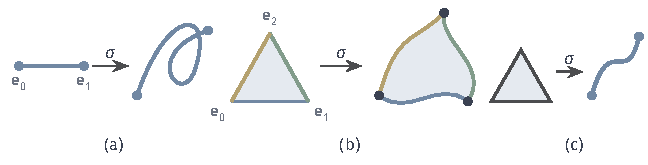
\includegraphics[width=109.657mm]{figures/04-spaces-measures-and-geometry/01-topology-and-metric/tikz/homol-singular-simplices/figure.pdf}
  \caption{奇异单形是连续映射，其像可以弯曲或退化。(a)$\sigma:\Delta^1\to X$是一条路径，允许自相交。(b)$\sigma:\Delta^2\to X$，蓝、绿、黄三条边是三个面$\sigma\circ\delta_2,\sigma\circ\delta_0,\sigma\circ\delta_1$的像。(c)$\Delta^2$可以被整个压到一条曲线上，它仍是一个合法的二维奇异单形。}
  \label{fig:homol-singular-simplices}
\end{BookInlineFigure}

$S_k(X)$通常是无穷维的：$X$中的每个点都是一个$0$维奇异单形，每条路径都是一个$1$维奇异单形，如图~\ref{fig:homol-singular-simplices}所示。但每个奇异链只涉及有限个奇异单形，所以下面的线性代数操作都是有限的。

\paragraph{奇异边界}
在复形中，$k$-单纯形的第$i$个面是去掉第$i$个顶点。对奇异单形，把它限制到$\Delta^k$的第$i$个面上即可。先用下面的映射把低一维的标准单纯形放到这个面上，它在第$i$个位置插入零：
\[
 \delta_i:\Delta^{k-1}\to\Delta^k,\qquad
 \delta_i(t_0,\ldots,t_{k-1})=(t_0,\ldots,t_{i-1},0,t_i,\ldots,t_{k-1}).
\]

这个映射把$\Delta^{k-1}$线性地送到$\Delta^k$中与$\bm e_i$相对的面上，并保持其余顶点的次序。奇异单形的边界就定义为
\begin{equation}
 \partial_k\sigma=\sum_{i=0}^k(-1)^i\,\sigma\circ\delta_i,
 \label{eq:homol-singular-boundary}
\end{equation}
线性延拓到$S_k(X)$。每个$\sigma\circ\delta_i$都是连续映射的复合，是$(k-1)$维奇异单形。对路径$\sigma$，
\[
 \partial_1\sigma=\sigma\circ\delta_0-\sigma\circ\delta_1=\sigma(\bm e_1)-\sigma(\bm e_0),
\]
仍是终点减起点。

\begin{example}[平面上一个奇异三角形的边界]
\label{ex:homol-singular-boundary}
取$X=\mathbb R^2$与线性映射
\[
 \sigma(t_0,t_1,t_2)=(t_1,t_2).
\]
它把$\Delta^2$送到顶点为$(0,0),(1,0),(0,1)$的三角形上，$\bm e_0,\bm e_1,\bm e_2$依次对应这三点。三个面依次是
\begin{align*}
 (\sigma\circ\delta_0)(s_0,s_1)&=\sigma(0,s_0,s_1)=(s_0,s_1),\\
 (\sigma\circ\delta_1)(s_0,s_1)&=\sigma(s_0,0,s_1)=(0,s_1),\\
 (\sigma\circ\delta_2)(s_0,s_1)&=\sigma(s_0,s_1,0)=(s_1,0).
\end{align*}
它们分别是从$(1,0)$到$(0,1)$、从$(0,0)$到$(0,1)$、从$(0,0)$到$(1,0)$的线段。由式~\eqref{eq:homol-singular-boundary}，
\[
 \partial_2\sigma=\sigma\circ\delta_0-\sigma\circ\delta_1+\sigma\circ\delta_2,
\]
正负号使三段路径沿三角形绕行一周，与单纯情形的$\partial_2[v_0,v_1,v_2]$一致。
\end{example}

\begin{lemma}[奇异边界的边界为零]
\label{lem:homol-singular-boundary-squared}
对$i<j$，作为$\Delta^{k-2}\to\Delta^k$的映射，
\begin{equation}
 \delta_j\circ\delta_i=\delta_i\circ\delta_{j-1}.
 \label{eq:homol-face-identity}
\end{equation}
因此$\partial_{k-1}\circ\partial_k=0$。
\end{lemma}

\begin{proof}
式~\eqref{eq:homol-face-identity}的两边都在第$i$与第$j$个位置插入零，其余坐标依次排在剩下的位置上。左边先在第$i$位插零，再在第$j$位插零。右边先在第$j-1$位插零，再在更靠前的第$i$位插零，使前一个零后移到第$j$位。所以两边相同。

展开两次边界，得到
\[
 \partial\partial\sigma=\sum_{j=0}^k\sum_{i=0}^{k-1}(-1)^{i+j}\sigma\circ\delta_j\circ\delta_i.
\]
按$i<j$与$i\geq j$分成两组。第一组用式~\eqref{eq:homol-face-identity}改写，再令$j'=j-1\geq i$，得到
\[
 \sum_{i<j}(-1)^{i+j}\sigma\circ\delta_i\circ\delta_{j-1}
 =-\sum_{i\leq j'}(-1)^{i+j'}\sigma\circ\delta_i\circ\delta_{j'}.
\]
第二组把求和字母改写为$a=j\leq b=i$，得到
\[
 \sum_{a\leq b}(-1)^{a+b}\sigma\circ\delta_a\circ\delta_b.
\]
两组逐项相消。
\end{proof}

这与定理~\ref{thm:homol-boundary-squared}是同一个机制：去掉两个顶点的两种先后次序以相反的符号出现。于是$(S_k(X),\partial_k)$是链复形。

\begin{definition}[奇异同调]
\label{def:homol-singular-homology}
拓扑空间$X$的$k$维（实系数）\term{奇异同调}（singular homology）空间定义为
\begin{equation}
 H_k(X)=\ker\partial_k/\operatorname{im}\partial_{k+1}.
 \label{eq:homol-singular-homology}
\end{equation}
闭链、边界链与同调类的说法与单纯情形相同。
\end{definition}

\begin{BookInlineTable}
  \centering
  \caption{单纯同调与奇异同调}
  \label{tab:homol-simplicial-vs-singular}
  \begin{tabular}{lll}
    \toprule
    & 单纯同调 & 奇异同调 \\
    \midrule
    输入 & 有限复形 & 任意拓扑空间 \\
    $k$维基向量 & $k$-单纯形，有限个 & 连续映射$\Delta^k\to X$ \\
    取边界 & 去掉第$i$个顶点 & 限制到第$i$个面 \\
    可否直接求秩 & 可以 & 不可以，维数无穷 \\
    是否依赖选择 & 依赖复形 & 只依赖空间 \\
    \bottomrule
  \end{tabular}
\end{BookInlineTable}

表~\ref{tab:homol-simplicial-vs-singular}比较了两种构造。奇异同调的优点和缺点恰好与单纯同调互补，第~\ref{sec:homol-simplicial-singular}小节要把二者接起来。

\paragraph{零维同调与路径分支}
零维奇异单形就是$X$中的点，一维奇异单形就是路径，其边界是终点减起点。所以零维同调的计算与定理~\ref{thm:homol-h0-components}平行，只是图的路径换成了空间中的路径。

\begin{theorem}[零维奇异同调计数路径分支]
\label{thm:homol-singular-h0}
设$X$的路径分支为$\{P_\alpha\}$，从每个$P_\alpha$中取一点$x_\alpha$。则$\{[x_\alpha]\}$是$H_0(X)$的一组基；特别地，$X$非空且路径连通时，$H_0(X)\cong\mathbb R$。
\end{theorem}

\begin{proof}
若$x,y$在同一路径分支中，取从$y$到$x$的路径$\sigma$，则$x-y=\partial_1\sigma$，二者同调。所以$\{[x_\alpha]\}$张成$H_0(X)$。

对每个分支$P_\alpha$定义线性函数$\varphi_\alpha$：把$0$维链在$P_\alpha$中各点上的系数相加。路径$\sigma$的像是路径连通集，起点与终点同属一个路径分支，所以$\varphi_\alpha(\partial_1\sigma)=0$，$\varphi_\alpha$在边界链上为零，在$H_0(X)$上有定义。

若有限组合$\sum\lambda_\alpha[x_\alpha]=0$，用$\varphi_\beta$作用得$\lambda_\beta=0$，所以它们线性无关。
\end{proof}

\paragraph{连续映射诱导的同调映射}
奇异同调的好处在于，任何连续映射都能直接作用在链上：奇异单形与连续映射复合，仍是奇异单形。单纯同调做不到这一点，一个连续映射通常不把单纯形送到单纯形。

\begin{theorem}[连续映射诱导同调映射]
\label{thm:homol-induced-map}
设$f:X\to Y$连续。令$f_\#\sigma=f\circ\sigma$并线性延拓，则$f_\#:S_k(X)\to S_k(Y)$是链映射，诱导线性映射$f_*:H_k(X)\to H_k(Y)$。并且$(\operatorname{id}_X)_*=\operatorname{id}$；若$g:Y\to Z$连续，则
\begin{equation}
 (g\circ f)_*=g_*\circ f_*.
 \label{eq:homol-functoriality}
\end{equation}
\end{theorem}

\begin{proof}
连续映射的复合满足结合律，所以
\[
 f\circ(\sigma\circ\delta_i)=(f\circ\sigma)\circ\delta_i.
\]
对式~\eqref{eq:homol-singular-boundary}逐项作用，得到
\[
 \partial f_\#\sigma=f_\#\partial\sigma,
\]
所以$f_\#$是链映射，由引理~\ref{lem:homol-chain-map-induces}诱导$f_*$。

在链层面，$(\operatorname{id}_X)_\#$是恒等映射，并且
\[
 (g\circ f)_\#\sigma=g\circ f\circ\sigma=g_\#f_\#\sigma,
\]
下降到同调即得后两条。
\end{proof}

若$f$是同胚，$f^{-1}$也连续，由式~\eqref{eq:homol-functoriality}，
\[
 f_*\circ(f^{-1})_*=(\operatorname{id}_Y)_*=\operatorname{id},
\]
另一侧同理，所以$f_*$是同构。同胚的空间有同构的奇异同调，Betti数是\term{拓扑不变量}（topological invariant）。反过来说，只要Betti数不同，两个空间就不同胚。

\subsection{单纯同调与奇异同调}
\label{sec:homol-simplicial-singular}

奇异同调对一切空间有定义，但$S_k(X)$是无穷维的，无法直接求秩。单纯同调能用有限矩阵计算，却依赖三角剖分。要把两者的长处结合起来，需要在有限复形上比较这两种链。

\paragraph{比较映射}
设$\mathcal K$是有限单纯复形，$V$上取定全序。一个单纯形可以直接看成一个奇异单形：把标准单纯形线性地放到它上面。对每个按递增次序排列的$k$-单纯形$[v_0,\ldots,v_k]$，令
\begin{equation}
 \theta[v_0,\ldots,v_k]:\Delta^k\to\lvert\mathcal K\rvert,\qquad(t_0,\ldots,t_k)\mapsto\sum_{i=0}^kt_i\bm e_{v_i},
 \label{eq:homol-comparison}
\end{equation}
这里$\bm e_{v_i}$是式~\eqref{eq:homol-realization}中顶点$v_i$对应的基向量。线性延拓，就得到链空间之间的映射
\[
 \theta:C_k(\mathcal K)\to S_k(\lvert\mathcal K\rvert).
\]

$\theta$只对递增排列的基向量定义。其他排列给出的奇异单形是同一个映射与坐标置换的复合，在$S_k$中是另一个基向量，并不等于它的$\pm1$倍；所以这里只能先固定定向，再线性延拓。

$\theta$是链映射。$\theta[v_0,\ldots,v_k]\circ\delta_i$在第$i$个坐标为零的点上取值，恰为$\theta[v_0,\ldots,\widehat{v_i},\ldots,v_k]$，而后者仍按递增次序排列。对式~\eqref{eq:homol-singular-boundary}与式~\eqref{eq:homol-boundary}逐项比较，符号$(-1)^i$也相同。所以$\partial\theta=\theta\partial$，由引理~\ref{lem:homol-chain-map-induces}，$\theta$诱导同调之间的线性映射$\theta_*$。

\begin{theorem}[单纯同调与奇异同调同构]
\label{thm:homol-simplicial-singular}
对有限单纯复形$\mathcal K$与一切$k$，
\begin{equation}
 \theta_*:H_k(\mathcal K)\to H_k(\lvert\mathcal K\rvert)
 \label{eq:homol-simplicial-singular}
\end{equation}
是同构。
\end{theorem}

这个定理的证明需要用到相对同调的长正合列、奇异链的重心细分（切除定理）与五引理，篇幅较长，读者可查阅代数拓扑教材中单纯同调与奇异同调等价的论证。这里说明它的含义与机制。

设想把复形一块一块搭起来，每次加入一个$k$-单纯形，它的边界已经在原来的复形里。这一步在两种同调上引起的变化相同：它只影响$k$维与$k-1$维，要么填掉一个$(k-1)$维的类，要么产生一个新的$k$维类，这由新单纯形的边界在旧复形中是否已是边界决定。证明的技术部分是说明奇异同调确实只“看到”这一块单纯形的相对信息，重心细分正是用来把任意奇异单形切小，切到每一小块都落在某个单纯形的邻域内。

逐块比较的结果是$\theta_*$在每一步都保持同构，从空复形出发归纳，就得到全部同构。

\paragraph{零维情形的核对}
在零维，定理~\ref{thm:homol-simplicial-singular}可以直接验证。由引理~\ref{lem:homol-simplices-intersect}，$\lvert\mathcal K\rvert$中每个点属于它的支撑所对应的凸包，凸包中的线段把它连到一个顶点；每条边的实现是连接两个端点的线段。所以一维骨架同一分量中的顶点在$\lvert\mathcal K\rvert$中属于同一路径分支，每个路径分支都含有顶点。

反过来，设$C$是一维骨架的一个分量，$\mathcal K_C$是顶点都在$C$中的单纯形组成的子复形。每个单纯形的顶点两两相邻，因而同属一个分量，所以$\lvert\mathcal K\rvert$是各个$\lvert\mathcal K_C\rvert$的不交并。

每个$\lvert\mathcal K_C\rvert$是有限个闭凸包之并，是闭集；它的补集是其余有限个闭集之并，也是闭集。这些闭集两两不交、并为整个空间，而一条路径的像是连通集，所以它只能落在其中一个之内。不同分量的顶点因而不在同一路径分支中。

于是两种零维同调都以“每个分量取一个顶点”为基，$\theta_*$把$[u_j]$送到$[u_j]$，是同构。

\paragraph{用三角剖分计算连续空间的同调}
定理~\ref{thm:homol-simplicial-singular}与同调的拓扑不变性合起来，给出计算连续空间同调的方法：找一个三角剖分$X\cong\lvert\mathcal K\rvert$，再按第~\ref{sec:homol-homology-spaces}小节求边界矩阵的秩。奇异同调不依赖任何选择，所以同一个空间的不同三角剖分必然给出同构的单纯同调。

\begin{example}[圆周、圆盘与球面的同调]
\label{ex:homol-sphere-homology}
由例~\ref{ex:homol-triangle-circle}，$S^1\cong\lvert\mathcal T_1\rvert$，$D^2\cong\lvert\mathcal T_2\rvert$，$S^2\cong\lvert\mathcal S\rvert$。由例~\ref{ex:homol-triangle-homology}与例~\ref{ex:homol-tetrahedron-homology}，
\[
 \begin{aligned}
 S^1&:\ \beta_0=\beta_1=1,\\
 D^2&:\ \beta_0=1,\\
 S^2&:\ \beta_0=1,\ \beta_1=0,\ \beta_2=1,
 \end{aligned}
\]
其余Betti数全为零。特别地，$S^1$与$S^2$不同胚，$S^1$与$D^2$也不同胚。
\end{example}

这些结论单从奇异同调的定义很难得到。例如$S^1$上有无穷多个从$\Delta^2$出发的连续映射，直接证明$H_2(S^1)=0$需要排除所有可能的奇异闭链。定理~\ref{thm:homol-simplicial-singular}把这一问题转化为三条边和三个顶点的矩阵计算。

\subsection{同伦不变性}
\label{sec:homol-homotopy-invariance}

第~\ref{sec:homol-homotopy}节说环带与圆周“有同样的洞”，却只能凭直观。现在可以证明：同伦的映射诱导相同的同调映射，因而同伦等价的空间有同构的同调。

\paragraph{棱柱构造}
设$H:X\times[0,1]\to Y$是从$f$到$g$的同伦。对$X$中的一条闭链$\bm z$，$H$把$\bm z\times[0,1]$扫成一块“柱面”，柱面的底是$f_\#\bm z$，顶是$g_\#\bm z$，见图~\ref{fig:homol-prism}(c)。若$\bm z$有边界，边界扫出侧面；$\bm z$闭合时没有侧面，于是$g_\#\bm z-f_\#\bm z$恰好是柱面的边界。

\begin{BookInlineFigure}
  \centering
  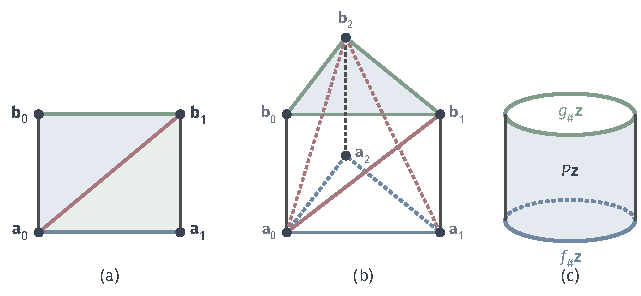
\includegraphics[width=108.511mm]{figures/04-spaces-measures-and-geometry/01-topology-and-metric/tikz/homol-prism/figure.pdf}
  \caption{棱柱的切分与同伦扫出的柱面。(a)$\Delta^1\times[0,1]$被红色对角线切成两个三角形，底边对应$f\circ\sigma$，顶边对应$g\circ\sigma$。(b)$\Delta^2\times[0,1]$被红色线段切成三个四面体$[\bm a_0,\bm b_0,\bm b_1,\bm b_2]$、$[\bm a_0,\bm a_1,\bm b_1,\bm b_2]$、$[\bm a_0,\bm a_1,\bm a_2,\bm b_2]$。(c)闭链$\bm z$被同伦扫成柱面，柱面的边界是顶$g_\#\bm z$减底$f_\#\bm z$。}
  \label{fig:homol-prism}
\end{BookInlineFigure}

要把这个柱面写成奇异链，需要把棱柱$\Delta^k\times[0,1]$切成若干个$(k+1)$维单纯形。记棱柱的底面顶点为$\bm a_i=(\bm e_i,0)$，顶面顶点为$\bm b_i=(\bm e_i,1)$，其中$i=0,\ldots,k$。

对棱柱中的点$\bm u_0,\ldots,\bm u_{k+1}$，记
\[
 \langle\bm u_0,\ldots,\bm u_{k+1}\rangle:\Delta^{k+1}\to\Delta^k\times[0,1]
\]
为把$\bm e_m$送到$\bm u_m$的线性映射，棱柱是凸集，所以它的像在棱柱中。对$X$中的奇异单形$\sigma$，令
\[
 F_\sigma=H\circ(\sigma\times\operatorname{id}_{[0,1]}):\Delta^k\times[0,1]\to Y,
\]
定义\term{棱柱算子}（prism operator）
\begin{equation}
 P\sigma=\sum_{i=0}^k(-1)^i\,F_\sigma\circ\langle\bm a_0,\ldots,\bm a_i,\bm b_i,\ldots,\bm b_k\rangle,
 \label{eq:homol-prism}
\end{equation}
它属于$S_{k+1}(Y)$，并线性延拓为$P:S_k(X)\to S_{k+1}(Y)$。

式中第$i$个单纯形从底面的前$i+1$个顶点出发，在第$i$个顶点处“爬上”顶面，再走完顶面的其余顶点。这$k+1$个单纯形拼成整个棱柱；下面的证明只用到它们的边界之间的相消关系。

\begin{example}[低维的棱柱]
\label{ex:homol-prism-low}
$k=0$时，$\sigma$是一点$x$，$P\sigma$是路径$t\mapsto H(x,t)$，边界为
\[
 \partial P\sigma=g(x)-f(x).
\]

$k=1$时，$\sigma$是路径，正方形$\Delta^1\times[0,1]$被对角线切成两个三角形：
\[
 P\sigma=F_\sigma\circ\langle\bm a_0,\bm b_0,\bm b_1\rangle-F_\sigma\circ\langle\bm a_0,\bm a_1,\bm b_1\rangle.
\]

省略复合号，按式~\eqref{eq:homol-singular-boundary}分别展开两项：
\begin{align*}
 \partial\bigl(F_\sigma\langle\bm a_0,\bm b_0,\bm b_1\rangle\bigr)&=F_\sigma\langle\bm b_0,\bm b_1\rangle-F_\sigma\langle\bm a_0,\bm b_1\rangle+F_\sigma\langle\bm a_0,\bm b_0\rangle,\\
 \partial\bigl(F_\sigma\langle\bm a_0,\bm a_1,\bm b_1\rangle\bigr)&=F_\sigma\langle\bm a_1,\bm b_1\rangle-F_\sigma\langle\bm a_0,\bm b_1\rangle+F_\sigma\langle\bm a_0,\bm a_1\rangle.
\end{align*}

两式相减，对角线$\langle\bm a_0,\bm b_1\rangle$相消，剩下
\[
 \partial P\sigma=F_\sigma\langle\bm b_0,\bm b_1\rangle+F_\sigma\langle\bm a_0,\bm b_0\rangle-F_\sigma\langle\bm a_1,\bm b_1\rangle-F_\sigma\langle\bm a_0,\bm a_1\rangle.
\]

四项依次是$g\circ\sigma$、起点的轨迹、终点的轨迹与$f\circ\sigma$。由于$\partial\sigma=\sigma(\bm e_1)-\sigma(\bm e_0)$，这正是
\[
 \partial P\sigma=g_\#\sigma-f_\#\sigma-P\partial\sigma,
\]
正方形的边界等于顶减底，再减去两条侧边。
\end{example}

例~\ref{ex:homol-prism-low}中的恒等式对一般的$k$也成立，图~\ref{fig:homol-prism}(a)(b)画出了$k=1,2$的切分。

\begin{lemma}[棱柱恒等式]
\label{lem:homol-prism-identity}
对一切$k\geq0$与$\sigma\in S_k(X)$，
\begin{equation}
 \partial P\sigma+P\partial\sigma=g_\#\sigma-f_\#\sigma.
 \label{eq:homol-prism-identity}
\end{equation}
\end{lemma}

\begin{proof}
记$[\cdots]$为$F_\sigma\circ\langle\cdots\rangle$，只需对奇异单形$\sigma$验证。对式~\eqref{eq:homol-prism}的第$i$项取边界，去掉第$j$个顶点：$j\leq i$时去掉的是$\bm a_j$，符号为$(-1)^j$；$j\geq i$时去掉的是$\bm b_j$，它位于第$j+1$个位置，符号为$(-1)^{j+1}$。于是$\partial P\sigma$是下面两组之和：
\begin{gather*}
 \sum_{j\leq i}(-1)^{i+j}[\bm a_0,\ldots,\widehat{\bm a_j},\ldots,\bm a_i,\bm b_i,\ldots,\bm b_k],\\
 \sum_{j\geq i}(-1)^{i+j+1}[\bm a_0,\ldots,\bm a_i,\bm b_i,\ldots,\widehat{\bm b_j},\ldots,\bm b_k].
\end{gather*}

先看$i=j$的项。第一组中$i=j$的项是$[\bm a_0,\ldots,\bm a_{i-1},\bm b_i,\ldots,\bm b_k]$，第二组中下标为$i-1$、去掉$\bm b_{i-1}$的项是它的相反数，因为符号为$(-1)^{2i-1}$。对$i=1,\ldots,k$，二者相消。剩下第一组$i=j=0$与第二组$i=j=k$的项：
\[
 [\bm b_0,\ldots,\bm b_k]=g\circ\sigma,\qquad-[\bm a_0,\ldots,\bm a_k]=-f\circ\sigma.
\]

再看$i\neq j$的项。去掉$\bm a_j$（$j<i$）或$\bm b_j$（$j>i$）后，剩下的单纯形恰好是第$j$个面$\sigma\circ\delta_j$所对应棱柱中的一块：前者是第$i-1$块，后者是第$i$块。这是因为$\delta_j\times\operatorname{id}$把较小棱柱的顶点按次序线性地送到这些顶点上，并满足
\[
 F_\sigma\circ(\delta_j\times\operatorname{id})=F_{\sigma\circ\delta_j}.
\]

按定义展开
\[
 P\partial\sigma=\sum_j(-1)^jP(\sigma\circ\delta_j)
 =\sum_{i>j}(-1)^{i+j-1}[\cdots\widehat{\bm a_j}\cdots]+\sum_{i<j}(-1)^{i+j}[\cdots\widehat{\bm b_j}\cdots],
\]
它恰好是$\partial P\sigma$中$i\neq j$各项的相反数。三部分相加，即得式~\eqref{eq:homol-prism-identity}。
\end{proof}

式~\eqref{eq:homol-prism-identity}的几何含义是：柱面的边界等于顶减底，再减去边界扫出的侧面。这是例~\ref{ex:homol-prism-low}中“正方形的边界”在一般维数上的写法。

\begin{theorem}[同伦不变性]
\label{thm:homol-homotopy-invariance}
若连续映射$f,g:X\to Y$同伦，则
\begin{equation}
 f_*=g_*:H_k(X)\to H_k(Y)
 \label{eq:homol-homotopy-invariance}
\end{equation}
对一切$k$成立。因此，若$f:X\to Y$是同伦等价，则$f_*$是同构；同伦等价的空间有同构的奇异同调。
\end{theorem}

\begin{proof}
对闭链$\bm z$，由引理~\ref{lem:homol-prism-identity}，
\[
 g_\#\bm z-f_\#\bm z=\partial P\bm z+P\partial\bm z=\partial P\bm z,
\]
右端是边界链，所以$g_*[\bm z]=f_*[\bm z]$。

若$h$是$f$的同伦逆，由定理~\ref{thm:homol-induced-map}与刚才的结论，
\[
 h_*f_*=(h\circ f)_*=(\operatorname{id}_X)_*=\operatorname{id},
\]
同理$f_*h_*=\operatorname{id}$，所以$f_*$是同构。
\end{proof}

这个结论称为同调的\term{同伦不变性}（homotopy invariance）。它在第~\ref{sec:homol-homotopy}节与本节之间架起桥梁：同伦等价保留的代数信息，至少包括全部Betti数。

\paragraph{单点与可缩空间}
单点空间$\{p\}$在每个维数恰有一个奇异单形$\sigma_k$（常值映射），并且$\sigma_k\circ\delta_i=\sigma_{k-1}$。由式~\eqref{eq:homol-singular-boundary}，
\[
 \partial_k\sigma_k=\sum_{i=0}^k(-1)^i\sigma_{k-1}=
 \begin{cases}0,&k\text{为奇数},\\ \sigma_{k-1},&k\geq2\text{为偶数}.\end{cases}
\]

所以$\partial_1=0$，$\partial_2$是同构，$\partial_3=0$，$\partial_4$是同构，依此类推。$k$为奇数时$\ker\partial_k=S_k$被$\operatorname{im}\partial_{k+1}$占满；$k\geq2$为偶数时$\ker\partial_k=0$。于是
\[
 H_0(\{p\})\cong\mathbb R,\qquad H_k(\{p\})=0\ (k\geq1).
\]
由定理~\ref{thm:homol-homotopy-invariance}，可缩空间（如区间、圆盘、$\mathbb R^n$）的同调与单点相同。

\paragraph{环带与圆周}
回到本章开头的问题。由例~\ref{ex:homol-annulus-retraction}与定理~\ref{thm:homol-retract-equivalence}，包含映射$i:S^1\to A$是同伦等价。由定理~\ref{thm:homol-homotopy-invariance}，$i_*$是同构，所以
\[
 H_1(A)\cong H_1(S^1)\cong\mathbb R.
\]
更具体地，环绕圆周一周的一维闭链，在环带中仍是不能填掉的闭链；环带比圆周多出的“厚度”被形变收缩压平，不产生新的同调类。

由此兑现第~\ref{sec:homol-homotopy-equivalence}小节的承诺：$H_1(A)\neq0=H_1(\{p\})$，所以环带不可缩。

同一论证还说明圆盘不能回缩到边界圆周上。若$r:D^2\to S^1$是回缩，$j:S^1\to D^2$为包含，则$r\circ j=\operatorname{id}_{S^1}$，于是$r_*\circ j_*$是$H_1(S^1)\cong\mathbb R$上的恒等映射。可是$j_*$经过$H_1(D^2)=0$，复合只能为零，矛盾。

\paragraph{同调不能判定什么}
同伦不变性同时划出了同调的边界。圆盘与单点同伦等价，同调相同，却不同胚；所以同调相同不能推出同胚，这一点在第~\ref{sec:homol-homology-spaces}小节已经用复形看到。

同调相同也不能推出同伦等价。环面与“两个圆周和一个球面粘在一点”的空间，Betti数都是$(1,2,1)$，却不同伦等价；区分它们要用基本群或同调环等更细的工具，证明需要另外建立这些工具。同调是检验“不同”的工具：Betti数不同，就足以断定两个空间既不同胚，也不同伦等价。

\section{本章小结}
\label{sec:homol-summary}

本章开头问：三角形框与三角形纸片有同样的顶点和边，怎样用代数量区分“有洞”与“被填上”；环带与圆周不同胚，怎样说明它们有同样的洞。前一个问题由单纯同调回答，后一个问题由同伦与同伦不变性回答。

同伦用乘积空间$X\times[0,1]$上的连续映射描述映射的连续变形，它是与复合相容的等价关系。把“互逆”放宽为“复合同伦于恒等映射”，得到同伦等价；与单点同伦等价的空间称为可缩空间，凸集都可缩。形变收缩把空间收回子空间并在过程中固定子空间，包含映射因而是同伦等价，环带由此与圆周同伦等价。同伦等价比同胚宽松：区间、圆盘和单点同伦等价，却两两不同胚。只有回缩而没有形变则不够，两点离散空间就是例子。

有限单纯复形用对取面封闭的顶点子集族记录点、边和各维填充，一维复形就是图。几何实现把每个单纯形换成标准单纯形，沿公共面粘合；它既是商空间，又同胚于欧氏空间中以标准基向量为顶点的凸包之并，其中两个单纯形只在公共面上相交。画在纸上的交叉不是复形中的点。

单纯同调在实数系数下取链空间$C_k(\mathcal K)\cong\mathbb R^{n_k}$，由交错取面定义边界映射，并验证$\partial\circ\partial=0$。闭链是边界映射的核，边界链是高一维边界映射的像，同调是二者之商，Betti数为$\beta_k=n_k-\operatorname{rank}\bm D_k-\operatorname{rank}\bm D_{k+1}$。$\beta_0$计数一维骨架的连通分量；三角形边界的$\beta_1=1$，填实后变为$0$；四面体表面的$\beta_2=1$。Euler示性数等于Betti数的交错和，可以核对手算。链映射诱导同调映射；比较子复形与大复形时，诱导映射能指出哪个环被填掉，单看Betti数做不到。

奇异同调以标准单纯形到空间的连续映射为基，对一切拓扑空间有定义，零维同调计数路径分支，连续映射诱导同调映射，同胚给出同构。在有限复形上，把单纯形看作线性的奇异单形，得到的比较映射在同调上是同构，本章只证明了零维情形并解释了一般机制；它使连续空间的同调可以用三角剖分的边界矩阵计算，并与三角剖分的选择无关。棱柱构造证明同伦映射诱导相同的同调映射，所以同伦等价的空间有同构的同调。由此，环带与圆周的$\beta_1$都是$1$，环带不可缩，圆盘不能回缩到边界圆周。

同调的使用有明确的方向：Betti数不同，就足以断定两个空间既不同胚，也不同伦等价；Betti数相同则什么也不能断定，圆盘与单点就是同调相同而不同胚的例子。流形上的同调在第~\ref{chap:manifold-basics}章起继续使用，从有限点云恢复同调、沿一列复形追踪诱导映射的持久同调在第~\ref{chap:manifold-recovery}章展开。下一部分转向另一类问题：不再研究连续变形与孔洞，而是在第~\ref{chap:measure}章度量集合的大小。


